\chapter{Erweiterte ToM+-Konfigurationen}

\section{Die WLAN-Einstellungsseite}
\label{sec:wifi_settings}

Seit dem zweiten Firmware-Release kann sich Ihr ToM+ über ein integriertes WLAN-Modul mit dem Internet verbinden. Dies ermöglicht es Ihnen, Ihre Twizy-Echtzeitdaten in Kombination mit dem MQTT-Protokoll anzuzeigen, das in Abschnitt~\ref{sec:MQTT} behandelt wird.\\

\begin{figure}[H]
    \centering
    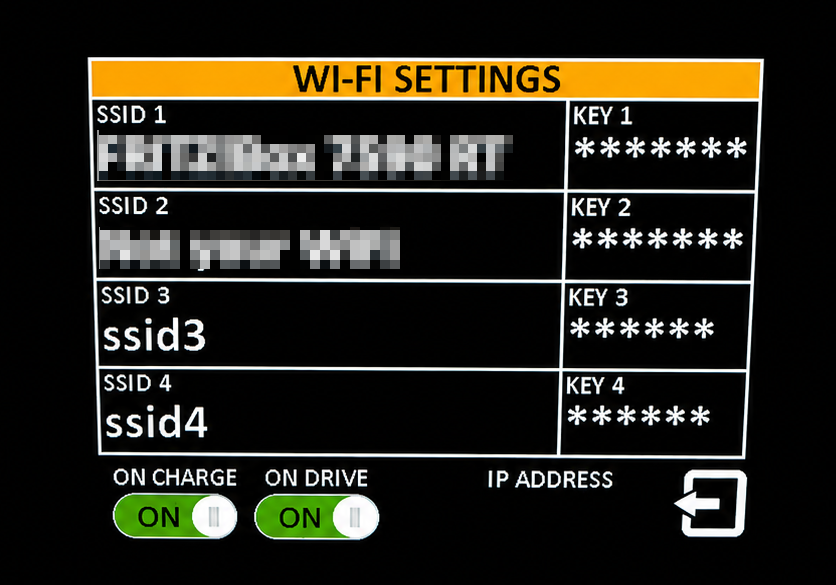
\includegraphics[width=0.8\textwidth]{figures/wifi_settings_3d.png}
    \caption{Die WLAN-Einstellungsseite.}
\end{figure}

Die Seite speichert bis zu vier Verbindungsprofile, um mit dem Internet verbunden zu sein, wenn Sie zu Hause, bei der Arbeit oder an einem öffentlichen Ort mit kostenlosem WLAN sind.\\
Zusätzlich verfügt ToM+ über eine Weboberfläche, auf der Sie Daten in Echtzeit überwachen oder Ihre Einstellungen viel einfacher anpassen können. Schauen wir uns nun an, warum Sie dies tun sollten…

\subsection{Vorteile von ToM+ WLAN}

Seit dem zweiten Firmware-Release kann sich Ihr ToM+ über ein integriertes WLAN-Modul mit dem Internet verbinden, was Ihnen den Zugriff auf viele weitere Funktionen als zuvor ermöglicht. Jetzt können Sie aus der Ferne auf Ihrem Smartphone auf Ihre Twizy-Daten zugreifen!\\

Sie müssen den Ladezustand Ihres Twizy nicht mehr manuell überprüfen, da diese neue Funktion die Daten zum Ladezustand direkt auf Ihrem Smartphone veröffentlicht, und diese sind sowohl geschützt als auch privat. Es erfordert lediglich eine kurze MQTT-Konfiguration.\\

\begin{itemize}
    \item Kein mühsames, manuelles Überprüfen des Twizy-Ladezustands mehr!
    \item Zahlreiche Möglichkeiten, Ihren Twizy über MQTT in ein IoT-System einzubinden
    \item WLAN beeinträchtigt weder den Stromverbrauch noch die ToM-Leistung merklich
    \item Schalten Sie eine neue Webseite mit Twizy-Echtzeitdaten und benutzerfreundlichen ToM-Einstellungen frei
\end{itemize}

\subsection{Hinzufügen eines WLAN-Verbindungsprofils}
\label{sec:add_wifi_profile}

Auf dieser neuen Einstellungsseite haben Sie eine kleine Tabelle mit vier Zeilen und zwei Spalten. Die erste Spalte enthält die \textbf{SSID} (d.~h. den Namen) des Netzwerks, mit dem Sie sich verbinden möchten. Um genau zu sein, ist es der Name, den Sie auf Ihrem Telefon oder Laptop sehen. Er kann alphanumerisch sein und unterscheidet zwischen Groß- und Kleinschreibung (Großbuchstaben sind wichtig, achten Sie also auf die korrekte Schreibweise!). Die zweite Spalte unter der Überschrift \textbf{„KEY“} ist für das WLAN-Passwort vorgesehen.\\

Wenn Sie auf eine Tabellenzelle tippen (entweder SSID oder Key), öffnet ToM+ eine Tastaturseite, auf der Sie Ihre Daten eingeben können. Das Drücken von OK bestätigt die eingegebene Zeichenfolge und führt Sie zurück zur WLAN-Einstellungsseite. Wir werden die Tastaturseite in Abschnitt~\ref{sec:keyboard_page} besprechen.\\

Bisher können Sie \textbf{vier verschiedene Verbindungsprofile} mit vier Paaren aus SSID und Passwort einrichten. Wenn Sie kein Profil einrichten, aber die WLAN-Schieberegler aktiviert sind, führt ToM+ dennoch alle zwei Minuten einen WLAN-Scan durch, um zu versuchen, öffentliche Verbindungen ohne Passwortschutz zu finden und sich dann zu verbinden. Drücken Sie die Taste mit dem \textbf{Pfeil unten rechts zum Speichern}.\\

Das vierte WLAN-Verbindungsprofil ist besonders, da das Feld \textbf{„KEY 4“} sowohl als Standard-Passwortfeld für die letzte SSID als auch zum Ändern des Standard-Webserver-Passworts verwendet wird, wie in Abschnitt~\ref{sec:web_change_password} besprochen wird.

Darüber hinaus gibt es einige Speziacodes, die Sie in dieses Feld eingeben können, um geheime Konfigurationen durchzuführen. Diese Codes unterscheiden zwischen Groß- und Kleinschreibung und wirken sich nicht auf Ihr Feld \textbf{„KEY 4“} aus, wenn sie korrekt geschrieben sind, da ToM+ sie nur als Befehle verwendet. Sie können \textbf{GIVE\textunderscore ME\textunderscore DF!} eingeben (exakt so wie hier geschrieben, auch mit Unterstrichen und Ausrufezeichen), um die \textit{DF-Fehlernummerierung und Fehlerbeschreibung} sowohl auf dem Display als auch in der Weboberfläche anzuzeigen.\\

\textbf{ERINNERUNG!} Die Befehle werden von ToM+ nur ausgeführt, wenn sie über diese WLAN-Einstellungsseite eingegeben werden, nicht über die später besprochene Weboberfläche. Da die Herkunft der DF-Nummer nicht eindeutig geklärt ist, erfolgt die Aktivierung dieser Funktion auf eigene Verantwortung.

\clearpage

\subsection{WLAN-Verbindung prüfen}
\label{sec:check_wifi_connection}

Die Überprüfung, ob Ihr ToM+ über WLAN mit dem Internet verbunden ist, ist sehr einfach. Auf allen Seiten befindet sich das WLAN-Symbol (behandelt in Abschnitt~\ref{sec:status_icon_bar}), das seinen Status anzeigt.

\iconbox{icons/Tray_WiFiOff.png}
{WLAN ist aus}
{ToM+ ist nicht verbunden und veröffentlicht keine Daten.}

\iconbox{icons/Tray_WiFi.png}
{WLAN ist an}
{ToM+ ist verbunden und veröffentlicht Daten, wenn MQTT verbunden ist.}

\iconbox{icons/Tray_WiFi.png}
{WLAN-Scan läuft}
{Wenn es blinkt, sucht ToM+ derzeit nach verfügbaren WLAN-Netzwerken.}

Wenn Sie spezifischere Informationen darüber erhalten möchten, ob Ihr ToM+ mit einem Netzwerk verbunden ist, können Sie zusätzliche Felder auf der WLAN-Einstellungsseite in der unteren rechten Ecke überprüfen, wie im folgenden Bild gezeigt.

\begin{figure}[H]
    \centering
    
\includegraphics[width=0.7\textwidth]{figures/wifi_bottom_line.png}
    \caption{Die WLAN-Info im unteren Raster.}
    \label{fig:wifi_bottom_line}
\end{figure}

Wie wir sehen können, wird eine IP-Adresse angezeigt, wenn ToM+ mit einem Netzwerk verbunden ist (hier ist es \textbf{10.24.126.204}). Dies ist die Adresse, die ToM+ verwendet, um sich mit dem Internet zu verbinden. Wenn dieses Feld eine Sequenz aus vier Zahlen (von 0 bis 255) enthält, die durch Punkte getrennt sind, ist WLAN verbunden; andernfalls bleibt es leer.

Tippen Sie darauf, um die MAC-Adresse von ToM+ anzuzeigen, und tippen Sie erneut, um zu sehen, mit welcher SSID (Netzwerkname) ToM+ verbunden ist. Weitere interessante Funktionen, bei denen die ToM+-IP-Adresse eine Rolle spielt, werden wir später in Abschnitt~\ref{sec:web_server_access} sehen.

\subsection{WLAN-Funktionen aktivieren/deaktivieren}
\label{sec:enable_disable_wifi}

In der Fußzeile der WLAN-Einstellungsseite befinden sich zwei Schieberegler. Um zwischen den Zuständen EIN und AUS zu wechseln, tippen oder schieben Sie sie einfach. Schauen wir uns an, was die beiden Schieberegler bewirken.\\

Der erste dient dazu, \textbf{WLAN beim Laden} zu deaktivieren. Dies führt dazu, dass Ihr ToM+ vollständig offline ist und Sie Ihre Twizy-Daten erst wieder aus der Ferne überwachen können, wenn Sie es erneut aktivieren. In diesem Zustand ist das WLAN-Statussymbol immer ausgegraut, wie in Abschnitt~\ref{sec:check_wifi_connection} gezeigt.\\

Der zweite Schieberegler dient zum Aktivieren von \textbf{WLAN beim Fahren}. Dies ermöglicht es Ihrem ToM+, auch während der Fahrt mit Ihrem Twizy mit dem Internet verbunden zu bleiben. Dies ist nützlich, wenn Sie Echtzeitdaten über MQTT auf Ihr Smartphone übertragen möchten. Dadurch wird auch der Zugriff auf die Weboberfläche während der Fahrt ermöglicht und ToM+ sucht ebenfalls nach verfügbaren WLAN-Netzwerken.\\

Wie bereits erwähnt, müssen Sie zum \textit{Speichern Ihrer Änderungen} die Pfeiltaste unten rechts drücken. Wenn Sie dies nicht tun, gehen Ihre Änderungen beim Verlassen der Seite verloren.

\clearpage

\section{Die MQTT-Einstellungsseite}
\label{sec:MQTT}

Wenn Sie bereits einen Blick auf den WLAN-Abschnitt~\ref{sec:wifi_settings} geworfen haben, wissen Sie wahrscheinlich bereits, dass MQTT erforderlich ist, um aus der Ferne auf Ihre Daten zuzugreifen. Dieser Abschnitt zeigt Ihnen, wie Sie es korrekt einrichten und wie die ToM+-Schnittstelle mit diesem Protokoll umgeht.

\begin{figure}[H]
    \centering
    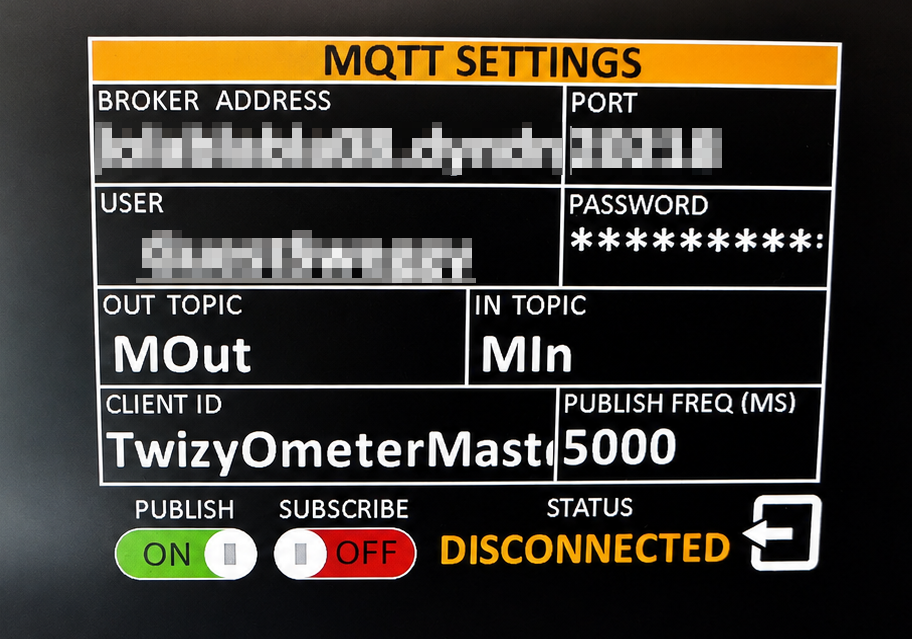
\includegraphics[width=0.8\textwidth]{figures/mqtt_settings_page.png}
    \caption{Die MQTT-Einstellungsseite.}
\end{figure}

Wenn ToM+ über WLAN mit dem Internet verbunden ist, kann MQTT aktiviert werden, und Sie können Ihre Twizy-Echtzeitdaten direkt auf Ihren Geräten anzeigen. Die Seite erlaubt nur eine MQTT-Serverkonfiguration, um \textbf{Datensicherheit und Privatsphäre} zu gewährleisten. Sie können diese Parameter sowohl auf dem ToM+ als auch auf seiner Webserver-Seite (Abschnitt~\ref{sec:web_network_settings}) konfigurieren. Besprechen wir nun, was MQTT ist und einige seiner Hauptvorteile…

\subsection{Kurze MQTT-Erklärung}
\label{sec:brief_mqtt}

MQTT ist eines der einfachsten Protokolle in der IT zur Übertragung kleiner Datennutzlasten mithilfe einer \textbf{Client/Server-Architektur}. Diese Methode erfordert einen oder mehrere Clients, die normalerweise Daten sammeln und diese dauerhaft speichern und/oder Berechnungen durchführen möchten.

Der Prozess benötigt also einen Server, der Daten von allen Clients verarbeitet und Aufgaben ausführt. Dieser Server wird als \textbf{MQTT-Broker} oder einfach Broker bezeichnet und ist in dieser Art von Architektur essenziell. Aber wie können Clients und Server untereinander kommunizieren?\\

Der Kommunikationsprozess basiert auf einer Publish/Subscribe-Struktur (Veröffentlichen/Abonnieren). Einige Clients sammeln und veröffentlichen Daten und werden aus diesem Grund \textbf{Publisher} genannt, während andere darauf warten, dass diese Daten gesendet werden, und als \textbf{Subscriber} bezeichnet werden. Der Broker-Server steht in der Mitte und ist das Vermittlungsgerät, auf dem alle Daten von Publishern gespeichert und an Subscriber gesendet werden. Führen wir nun Topics ein…\\

Ein \textbf{Topic} ist eine Abfolge von alphanumerischen Zeichen, die sich typischerweise auf ein bestimmtes Thema bezieht und dazu dient, alle Daten zu diesem spezifischen Thema zu speichern (wie ein Container). Topics sind nützlich, um eine Vielzahl von Daten zu organisieren, die von verschiedenen Publishern gesammelt wurden, um diese Informationen nicht zu verwirren. Wie nutzt ToM+ also MQTT?

\subsection{ToM+ und MQTT-Kommunikation}

Nachdem wir nun wissen, was MQTT ist, wollen wir sehen, wie das MQTT- und ToM+-System tatsächlich funktioniert. ToM+ gilt als Publisher, da es aktualisierte Twizy-Daten sammelt und veröffentlicht. Die Smartphone-Anwendung hingegen ist der Subscriber, da sie darauf wartet, diese vom Twizy eben veröffentlichten Daten zu empfangen. Wer steht in der Mitte? Der Broker-Server.\\

Sofern Sie keinen selbst gehosteten Broker-Server haben (wie ich) oder bereits einen kennen, den Sie nutzen können, erkläre ich in Abschnitt~\ref{sec:free_broker}, wie Sie Ihren kostenlosen externen Broker-Server einrichten.

Die Kombination von ToM+ mit dem MQTT-Protokoll kann sehr leistungsfähig sein, und wenn Sie Heimautomatisierung und IoT-Systeme mögen, eröffnen sich unendliche Möglichkeiten. Sie können beispielsweise Ihren eigenen Subscriber erstellen, der Aktionen auf Basis der von ToM+ veröffentlichten Daten ausführt.\\

\subsection{Einrichten eines kostenlosen MQTT-Brokers}
\label{sec:free_broker}

\textit{Haftungsausschluss}: Nehmen Sie sich Zeit für diesen Vorgang, da er für nicht erfahrene Benutzer einige Minuten länger dauern kann, und stellen Sie sicher, dass Sie sich Ihre \textbf{Konfigurationsparameter notieren}.\\

Wählen Sie zuallererst Ihren MQTT-Broker-Anbieter. Ich persönlich empfehle Maqiatto, da es kostenlos, intuitiv und einfach zu bedienen ist. Besuchen wir also die Tutorial-Seite der offiziellen Website: \url{https://www.maqiatto.com/examples}. Nun sollten wir eine Seite sehen, wie sie hier gezeigt wird:

\begin{figure}[H]
    \centering
    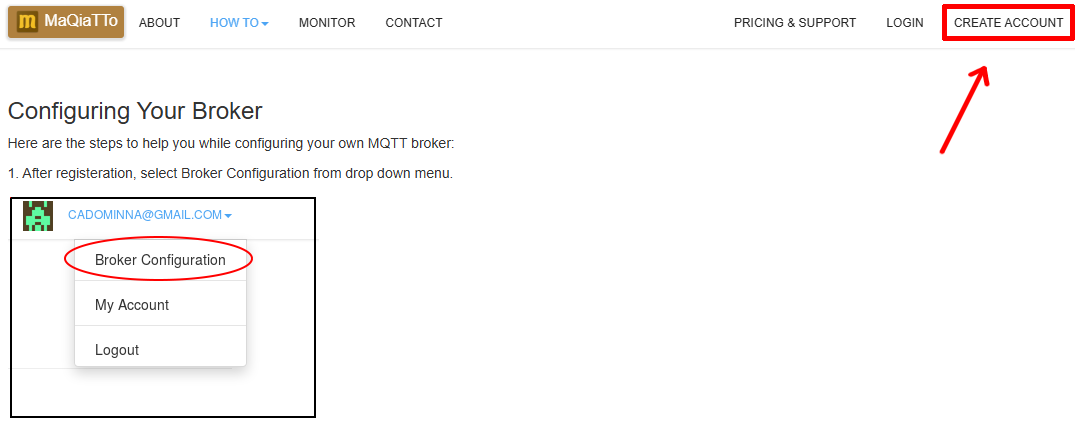
\includegraphics[width=1\textwidth]{figures/mqtt_step1.png}
    \caption{Schritt 1: Drücken Sie die Taste „CREATE ACCOUNT“.}
\end{figure}

Wie in der offiziellen Anleitung beschrieben, benötigen Sie ein Konto, um Ihren MQTT-Broker zu erstellen. Drücken Sie also die oben rechts eingekreiste Taste \textbf{„Create Account“} und erstellen Sie ein Konto. Sie werden zu dieser Seite weitergeleitet (\url{https://www.maqiatto.com/signup}), auf der Sie Ihre persönlichen Daten eingeben müssen.

\begin{figure}[H]
    \centering
    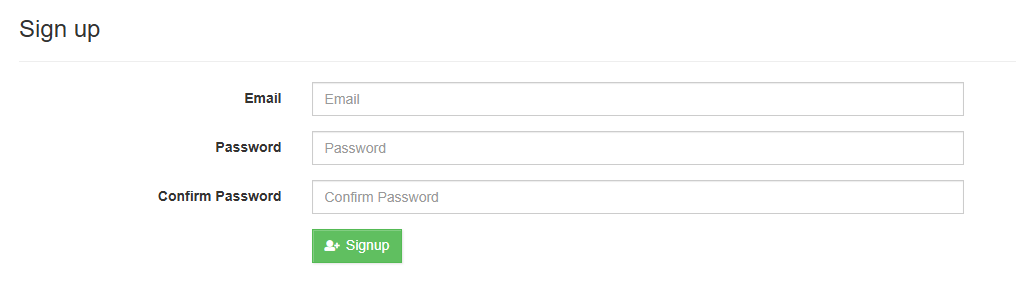
\includegraphics[width=1\textwidth]{figures/mqtt_step2.png}
    \caption{Schritt 2: Füllen Sie Ihre persönlichen Daten aus.}
\end{figure}

Nachdem Sie alle Formularfelder ausgefüllt haben, drücken Sie die grüne Taste \textbf{„Signup“} und warten Sie, bis diese Seite (\url{https://www.maqiatto.com/configure}) mit einer Erfolgsmeldung für die Registrierung erscheint, wie im Bild unten gezeigt:

\begin{figure}[H]
    \centering
    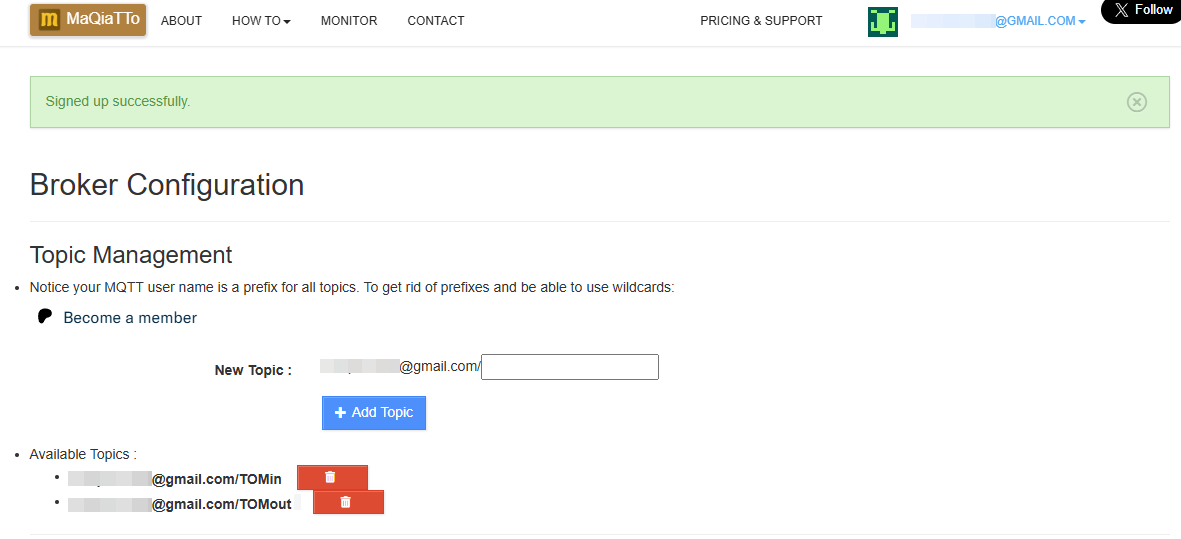
\includegraphics[width=1\textwidth]{figures/mqtt_step3.png}
    \caption{Schritt 3: IN/OUT-Topics hinzufügen.}\label{sec:free_broker_add_topics}
\end{figure}

Auf dieser Seite können Sie Ihre verfügbaren Topics verwalten (siehe Abschnitt~\ref{sec:brief_mqtt}) und neue erstellen. Erstellen wir also unser IN- und OUT-Topic zum Senden und Empfangen von ToM-Daten. Wie wir sehen können, gibt es ein festes Präfix (Ihre E-Mail-Adresse), da kostenlose Benutzer dieser Einschränkung unterliegen, aber das ist überhaupt kein Problem.\\

In das leere Textfeld nach dem „/“-Symbol sollten wir den Namen eintragen, den wir unseren Topics geben möchten. Wählen Sie ihn sorgfältig aus und stellen Sie sicher, dass er klar und leicht zu merken ist. Ich werde das Eingabe-Topic beispielsweise \textbf{TOMin} und das Ausgabe-Topic \textbf{TOMout} nennen, aber Sie können den Namen wählen, den Sie bevorzugen.\\

Geben Sie für das erste Topic \textbf{TOMin} ein und drücken Sie die blaue Taste \textbf{„+ Add Topic“}, wie ich es oben getan habe. Wenn der Vorgang erfolgreich abgeschlossen ist, wird eine grüne Pop-up-Meldung angezeigt mit dem Text \textbf{„Topic was added for this user“} und ein neuer Eintrag erscheint in der Liste der \textit{„Available Topics“}, die zuvor leer war. Wiederholen Sie den Vorgang nun auch für das Topic \textbf{TOMout} und überprüfen Sie erneut, ob das Topic erfolgreich erstellt wurde. Vor diesem Vorgang war die Liste der \textit{„Available Topics“} leer, aber jetzt können wir unsere beiden Topics in der Liste sehen und sie bei Bedarf löschen.

\begin{figure}[H]
    \centering
    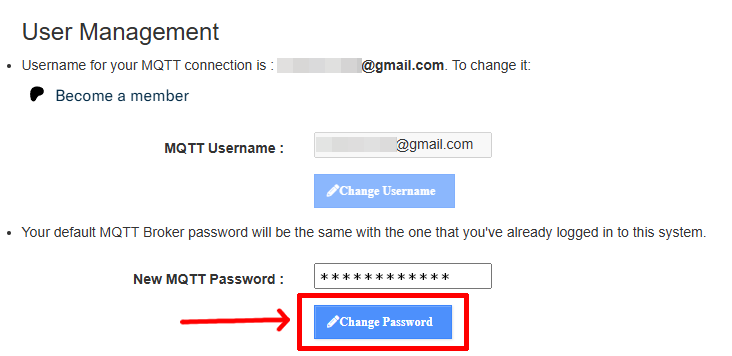
\includegraphics[width=0.8\textwidth]{figures/mqtt_step4.png}
    \caption{Schritt 4: Ändern Sie Ihr Broker-Passwort.}
\end{figure}

\textit{Dieser Schritt wird empfohlen, ist jedoch optional}. Zu diesem Zeitpunkt entspricht das Broker-Passwort dem Ihres Maqiatto-Kontos und ist überhaupt nicht sicher. Wenn Sie es jedoch nicht ändern möchten oder es Ihnen egal ist, können Sie diesen Schritt überspringen und zum nächsten übergehen.\\

Nehmen wir uns also etwas Zeit, um den Broker sicher zu machen und vor unbefugtem Zugriff zu schützen. Der zweite Teil dieser Seite (\url{https://www.maqiatto.com/configure}) ermöglicht es Ihnen, Ihr Broker-Passwort zu ändern. Geben Sie einfach das neue Passwort in das Textfeld \textbf{„New MQTT Password“} ein und drücken Sie dann die blaue Taste \textbf{„Change Password“}.

Wenn alles klappt, erscheint eine grüne Pop-up-Meldung mit dem Text \textbf{„Broker user password was updated“}. Die Taste zum Ändern des Benutzernamens ist ausgegraut, da Sie Ihren Benutzernamen nur ändern können, wenn Sie Premium-Benutzer sind.

\begin{figure}[H]
    \centering
    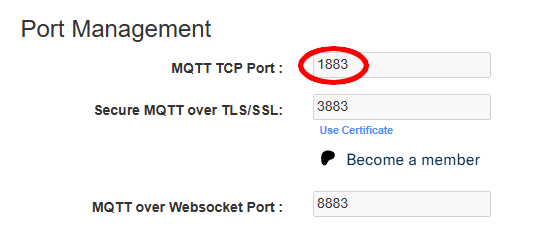
\includegraphics[width=0.7\textwidth]{figures/mqtt_step5.png}
    \caption{Schritt 5: Notieren Sie sich die Portnummer.}
\end{figure}

Im letzten Abschnitt der Konfigurationsseite (\url{https://www.maqiatto.com/configure}) befinden sich die \textbf{„Port Management“}-Parameter. Notieren Sie sich den MQTT-TCP-Port, der gewöhnlich auf \textbf{1883} eingestellt ist (nur um sicherzugehen), da dies die Standard-Portnummer im Internet für das MQTT-Protokoll ist. Nun ist der MQTT-Broker bereit zur Verwendung und wir können zum nächsten Schritt übergehen: der Konfiguration von ToM+ mit den Broker-Parametern.

\clearpage

\subsection{ToM+ mit dem MQTT-Broker verbinden}
\label{sec:mqtt_connection}

Nachdem nun klar ist, was MQTT ist (Abschnitt~\ref{sec:brief_mqtt}), und wir unseren persönlichen Broker eingerichtet haben (Abschnitt~\ref{sec:free_broker}), wollen wir sehen, wo auf dem Display wir ToM+ mit unserem frisch erstellten Broker verbinden können.

\begin{figure}[H]
    \centering
    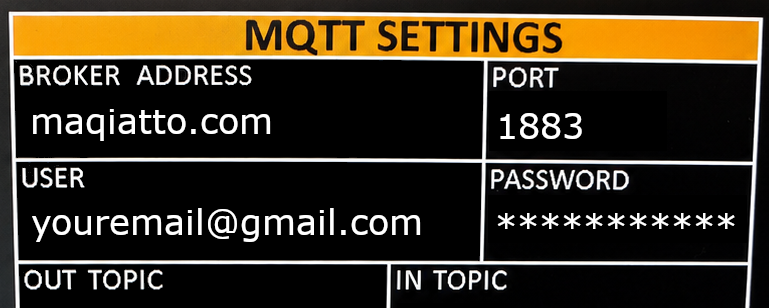
\includegraphics[width=0.8\textwidth]{figures/mqtt_connect1.png}
    \caption{MQTT-Broker-Verbindungsparameter.}
\end{figure}

Wenn Sie auf das entsprechende Tabellenfeld tippen, öffnet ToM+ eine Tastaturseite, auf der Sie Ihre Daten eingeben können, wie in den WLAN-Einstellungen. Um Symbole oder Zahlen einzugeben, drücken Sie die Taste \textbf{„1/3“} auf der Tastatur, um den Zeichensatz zu wechseln. Durch Drücken von \textbf{OK} bestätigen Sie die eingegebene Zeichenfolge und kehren zur MQTT-Einstellungsseite zurück. Weitere Informationen zur Tastaturseite finden Sie in Abschnitt~\ref{sec:keyboard_page}. Wenn der Wert zu lang für das Feld ist, scrollt der Text automatisch.\\

Als Erstes müssen Sie Ihre \textbf{Broker-Adresse} angeben. Im gezeigten Beispiel ist sie auf \textit{„maqiatto.com“} eingestellt. Dies ist die Adresse des Broker-Servers, den wir gerade in Abschnitt~\ref{sec:free_broker} erstellt haben.

Anschließend muss die \textbf{Portnummer} angegeben werden, auf der der MQTT-Dienst läuft. Sofern Sie sie nicht manuell auf eine andere Nummer eingestellt haben, ist der MQTT-Port immer \textit{1883}.

Als Nächstes folgt das Feld \textbf{User}, das den Benutzernamen darstellt, den ToM+ zur Authentifizierung bei der Verbindung mit dem Broker verwendet. Da das Paar aus Benutzername und Passwort einzigartig für Sie ist, verhindert dies, dass unerwünschte Benutzer Zugriff auf Ihren privaten Broker erhalten. In Ihrem Fall ist der Benutzer die E-Mail-Adresse Ihres Maqiatto-Kontos, geschrieben wie \textit{youremail@example.com}.

Danach müssen wir das \textbf{Passwort des Brokers} angeben, das sich von dem Ihres Maqiatto-Kontos unterscheiden kann, wenn Sie es wie in Abschnitt~\ref{sec:free_broker} empfohlen geändert haben.

\begin{figure}[H]
    \centering
    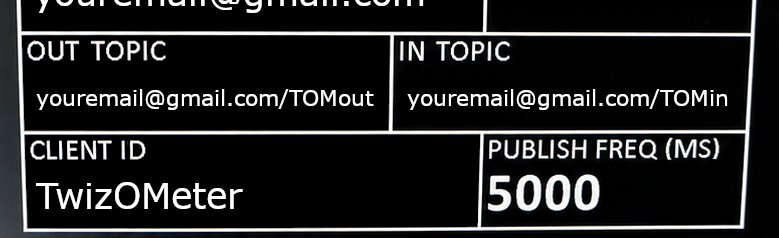
\includegraphics[width=0.8\textwidth]{figures/mqtt_connect2.png}
    \caption{MQTT ToM+ Veröffentlichungsparameter.}
\end{figure}

Konfigurieren wir nun unser \textbf{OUT-Topic}, in dem ToM+ die Twizy-Daten veröffentlichen wird. In Abschnitt~\ref{sec:free_broker} haben wir ein Out-Topic namens TOMout erstellt, aber der vollständige Name des Topics muss auch \textbf{Ihre E-Mail-Adresse als Präfix} enthalten, gefolgt von einem „/“-Symbol und dem Topic-Namen „TOMout“. Im Beispiel ist es auf \textit{„youremail@gmail.com/TOMout“} eingestellt.

Jetzt ist es Zeit für das \textbf{IN-Topic}, über das ToM+ MQTT-Befehle empfängt. Wie beim OUT-Topic haben wir ein In-Topic namens TOMin erstellt, aber der vollständige Name des Topics muss auch \textbf{Ihre E-Mail-Adresse als Präfix} enthalten, gefolgt von einem „/“-Symbol und dem Topic-Namen „TOMin“. Im Beispiel ist es auf \textit{„youremail@gmail.com/TOMin“} eingestellt.

Wenn ein MQTT-Publisher eine Nachricht an den Broker sendet, wird seine Verbindung durch Benutzername und Passwort authentifiziert, aber er veröffentlicht unter einem Alias, den Sie \textit{willkürlich wählen können}. Es ist wichtig, keine Leerzeichen in der \textbf{Client ID} zu verwenden; es sind nur alphanumerische Zeichen und Symbole erlaubt. Denken Sie daran, dass es ratsam ist, diese einfach und klar zu halten, wie im Beispiel: \textit{„TwizOMeter“}.

Der letzte Parameter ist die \textbf{Veröffentlichungsfrequenz} (Publish Frequency), die die Zeit zwischen den einzelnen ToM+-Veröffentlichungen darstellt. Sie wird in Millisekunden \textit{(ms)} ausgedrückt und kann auf einen beliebigen Wert größer als 1000 ms (eine Sekunde) eingestellt werden. Der Standardwert beträgt \textit{5000 ms} (fünf Sekunden) und stellt einen guten Kompromiss zwischen Datenaktualität und Netzwerkauslastung dar.\\

Um Ihre \textbf{Änderungen zu speichern}, müssen Sie die Pfeiltaste unten rechts drücken. Wenn Sie dies nicht tun, gehen Ihre Änderungen beim Verlassen der Seite verloren. Nun ist ToM+ bereit, Daten über das MQTT-Protokoll zu senden und zu empfangen.\\

\subsection{MQTT-Funktionen aktivieren/deaktivieren}
\label{sec:enable_disable_mqtt}

Wenn Sie das Veröffentlichen von Daten mit dem MQTT-Protokoll vorübergehend oder dauerhaft deaktivieren möchten, drücken oder schieben Sie den linken Schieberegler mit der Aufschrift \textbf{„PUBLISH“} im Bild unten. Von da an wird ToM+ keine Twizy-Daten mehr über MQTT veröffentlichen, bis Sie es wieder aktivieren.

\begin{figure}[H]
    \centering
    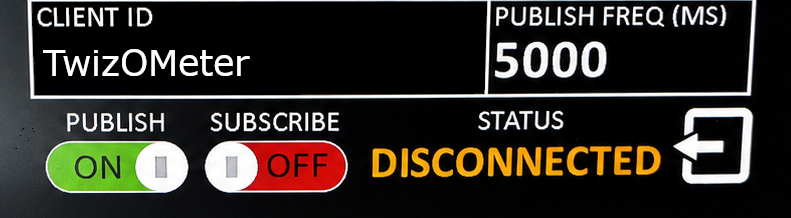
\includegraphics[width=0.8\textwidth]{figures/mqtt_connect3.png}
    \caption{Untere MQTT-Schieberegler.}
\end{figure}

Der rechte Schieberegler unter \textbf{„SUBSCRIBE“} ermöglicht es ToM+, Befehle von externen Geräten zu empfangen, die auf dem angegebenen IN-Topic veröffentlicht werden. Dies ist nützlich, wenn Sie ein an den ToM+-Erweiterungsanschluss angeschlossenes Gerät über MQTT steuern möchten (z.~B. eine smarte Steckdose zum Ferneinschalten des Ladevorgangs). Sie können diese Funktion jederzeit aktivieren oder deaktivieren, indem Sie die Taste drücken oder schieben.\\

\subsection{ToM+ MQTT-Verbindung prüfen}

Neben den beiden Schiebereglern befindet sich ein kleines \textbf{„STATUS“}-Feld, das anzeigt, ob die MQTT-Verbindung funktioniert oder nicht. Wenn ToM+ mit dem angegebenen MQTT-Broker verbunden ist, sehen Sie den Text \textit{„CONNECTED“}. Wenn ein Problem mit der Broker-Verbindung vorliegt oder WLAN deaktiviert ist (wie in Abschnitt~\ref{sec:enable_disable_wifi} gesehen), funktioniert MQTT nicht ordnungsgemäß und es erscheint die Meldung \textit{„DISCONNECTED“}, wie im Bild unten gezeigt.

\begin{figure}[H]
    \centering
    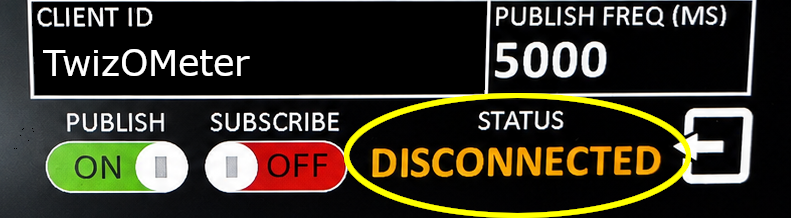
\includegraphics[width=0.8\textwidth]{figures/mqtt_status.png}
    \caption{MQTT-Statusfeld.}
\end{figure}

Übrigens können Sie den MQTT-Verbindungsstatus auch überprüfen, indem Sie auf die Status-Symbolleiste schauen (Abschnitt~\ref{sec:status_icon_bar}), in der das MQTT-Symbol lila ist, wenn die Verbindung hergestellt ist, andernfalls ist es ausgegraut.

Um Ihre \textbf{Änderungen zu speichern}, müssen Sie die Pfeiltaste unten rechts drücken. Wenn Sie dies nicht tun, gehen Ihre Änderungen beim Verlassen der Seite verloren.\\


\section{Die Tastaturseite}
\label{sec:keyboard_page}

Wenn Sie in der WLAN- oder MQTT-Einstellungsseite auf eine Tabellenzelle tippen, öffnet ToM+ eine Tastaturseite, auf der Sie Ihre Daten eingeben können. Die Tastaturseite ist sehr intuitiv und einfach zu bedienen. Sie können zwischen drei verschiedenen Zeichensätzen wechseln, indem Sie die Taste \textbf{„1/3“} in der unteren linken Ecke der Tastatur drücken.

\begin{figure}[ht]
    \centering

    \begin{subfigure}[t]{0.48\textwidth}
        \centering
        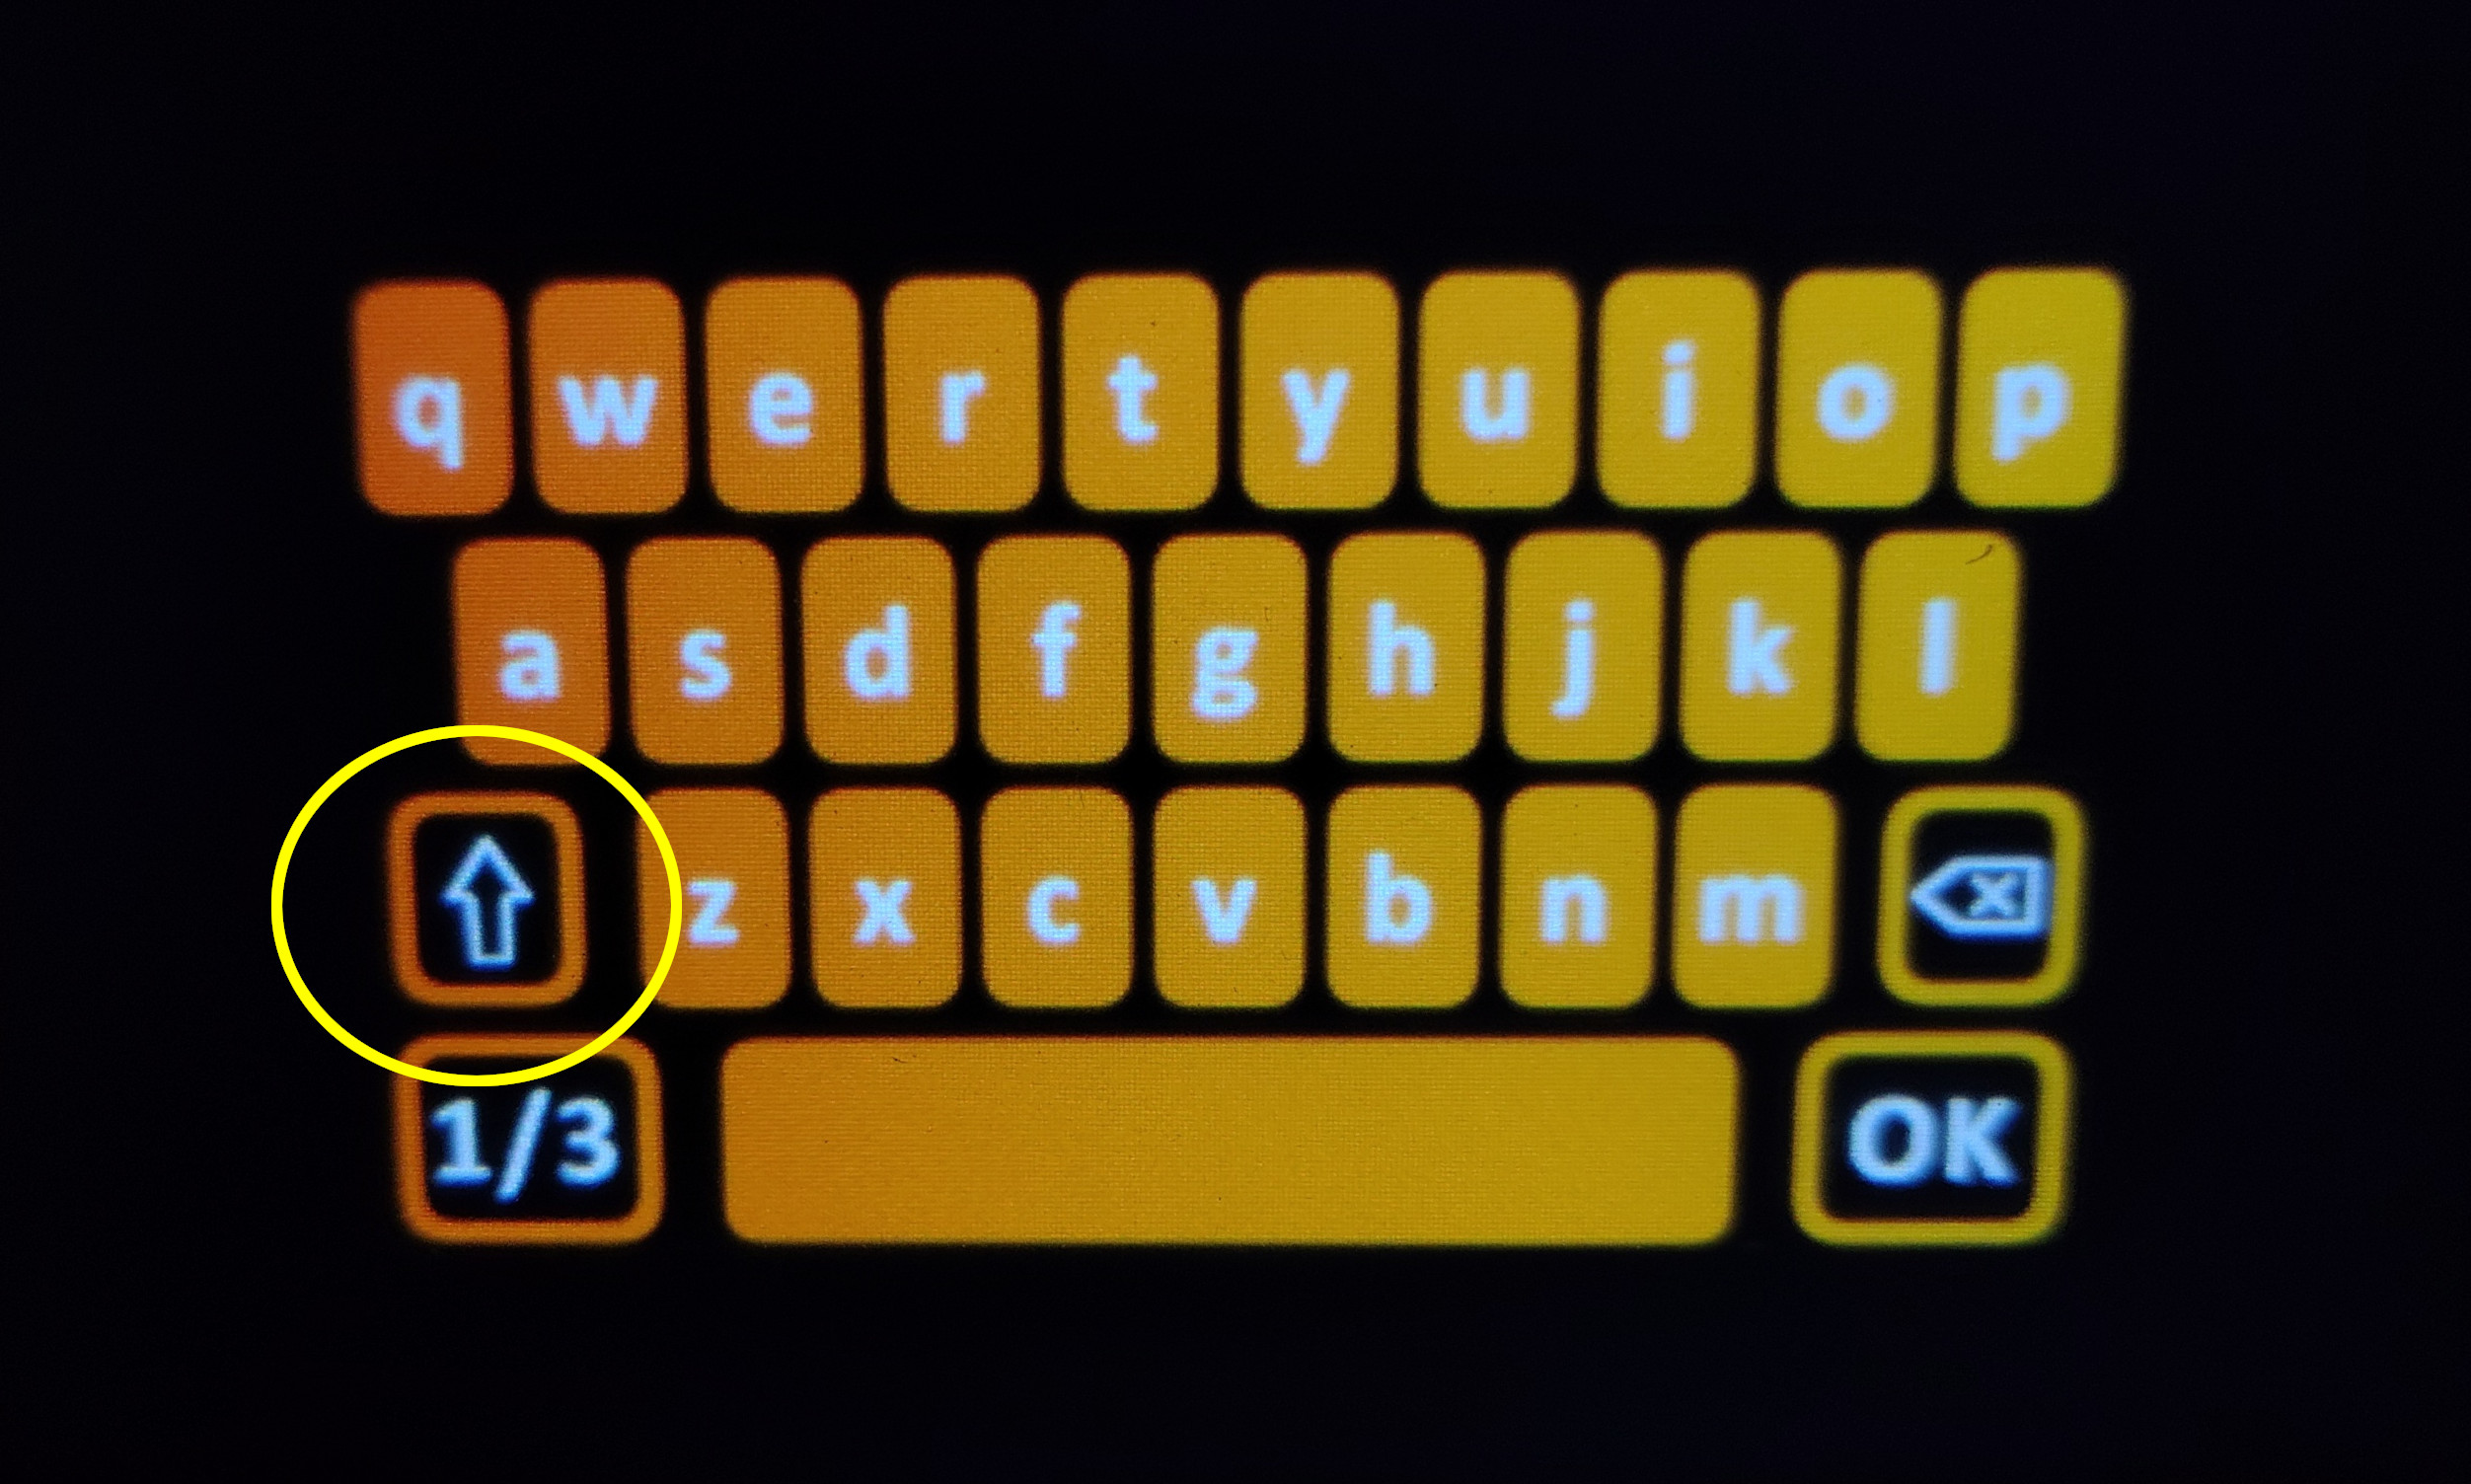
\includegraphics[width=\linewidth]{figures/keyboard_page1.jpg}
        \caption{Erster Zeichensatz: Buchstaben.}
    \end{subfigure}
    \hfill
    \begin{subfigure}[t]{0.48\textwidth}
        \centering
        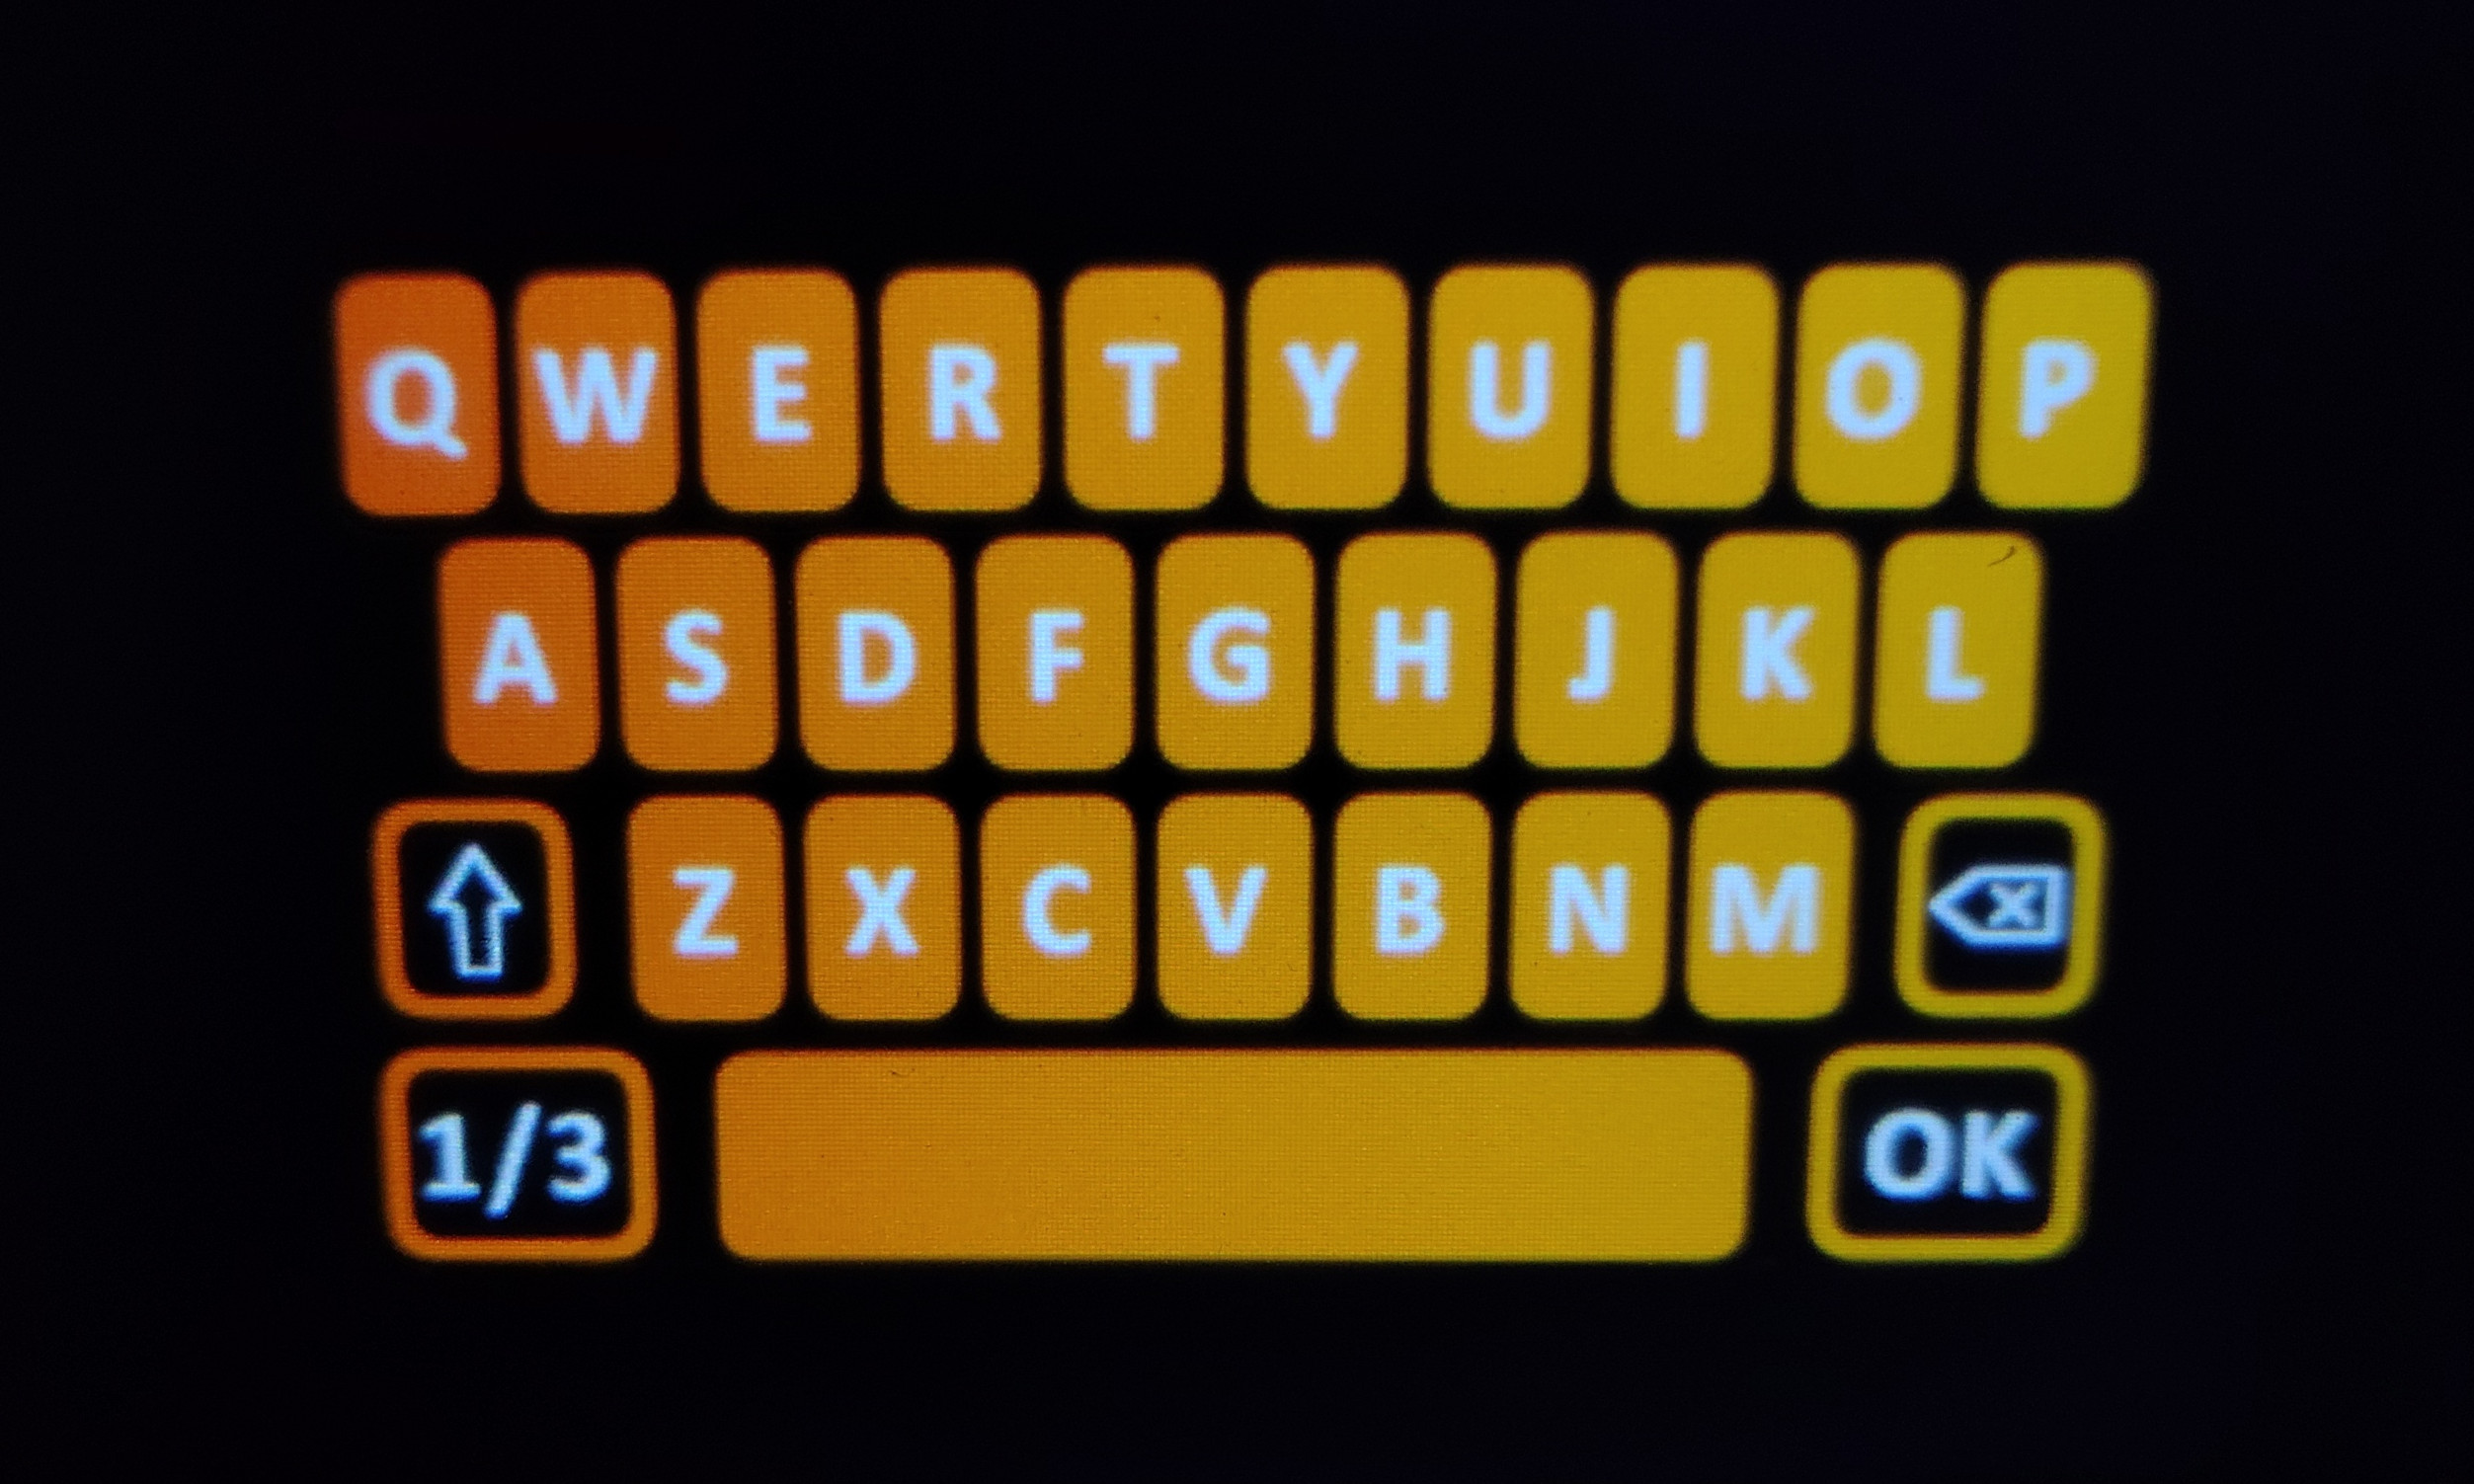
\includegraphics[width=\linewidth]{figures/keyboard_page1_caps.jpg}
        \caption{Erster Zeichensatz: Großbuchstaben.}
    \end{subfigure}
\end{figure}

Im \textbf{ersten Zeichensatz} können Sie Buchstaben in Klein- oder Großschreibung eingeben, indem Sie die im ersten Bild gelb eingekreiste Shift-Taste drücken.
Wenn Sie etwas eingeben, erscheint es im Textfeld oben auf der Tastatur. Wenn Sie ein Zeichen löschen möchten, drücken Sie einfach die Rücktaste (Backspace).

\clearpage

\begin{figure}[ht]
    \centering

    \begin{subfigure}[t]{0.48\textwidth}
        \centering
        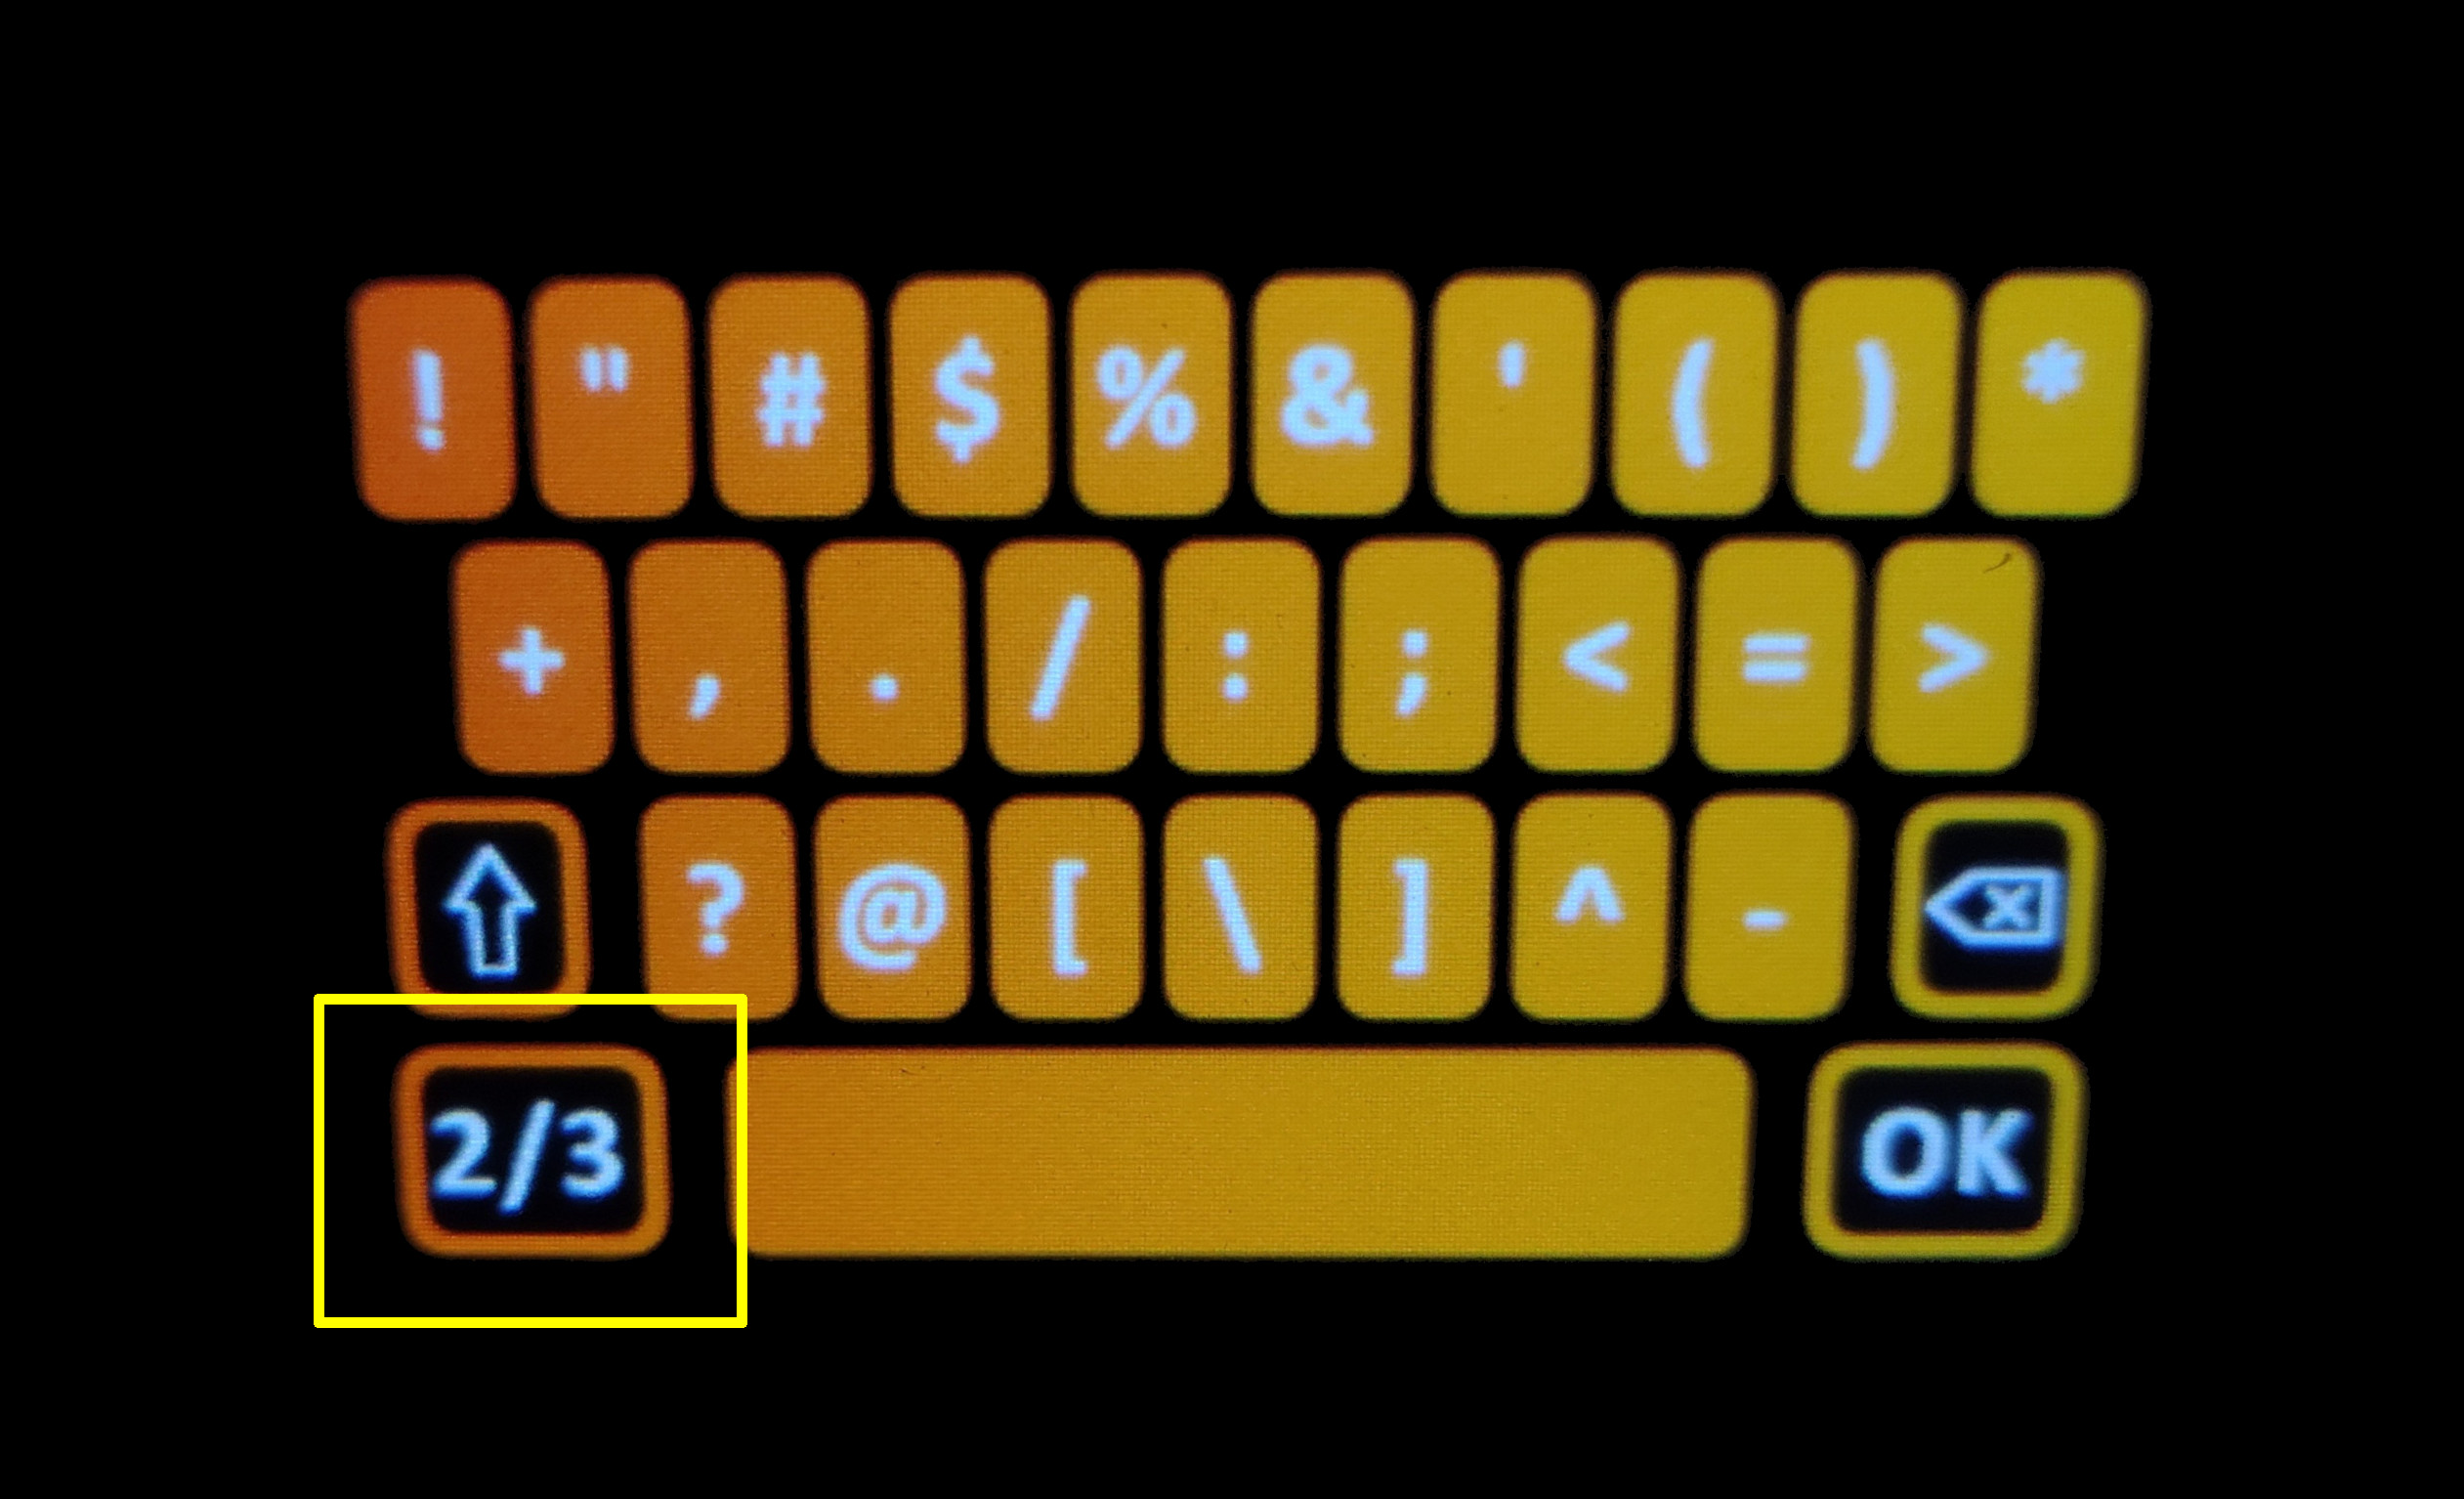
\includegraphics[width=\linewidth]{figures/keyboard_page2.jpg}
        \caption{Zweiter Zeichensatz: Symbole.}
    \end{subfigure}
    \hfill
    \begin{subfigure}[t]{0.48\textwidth}
        \centering
        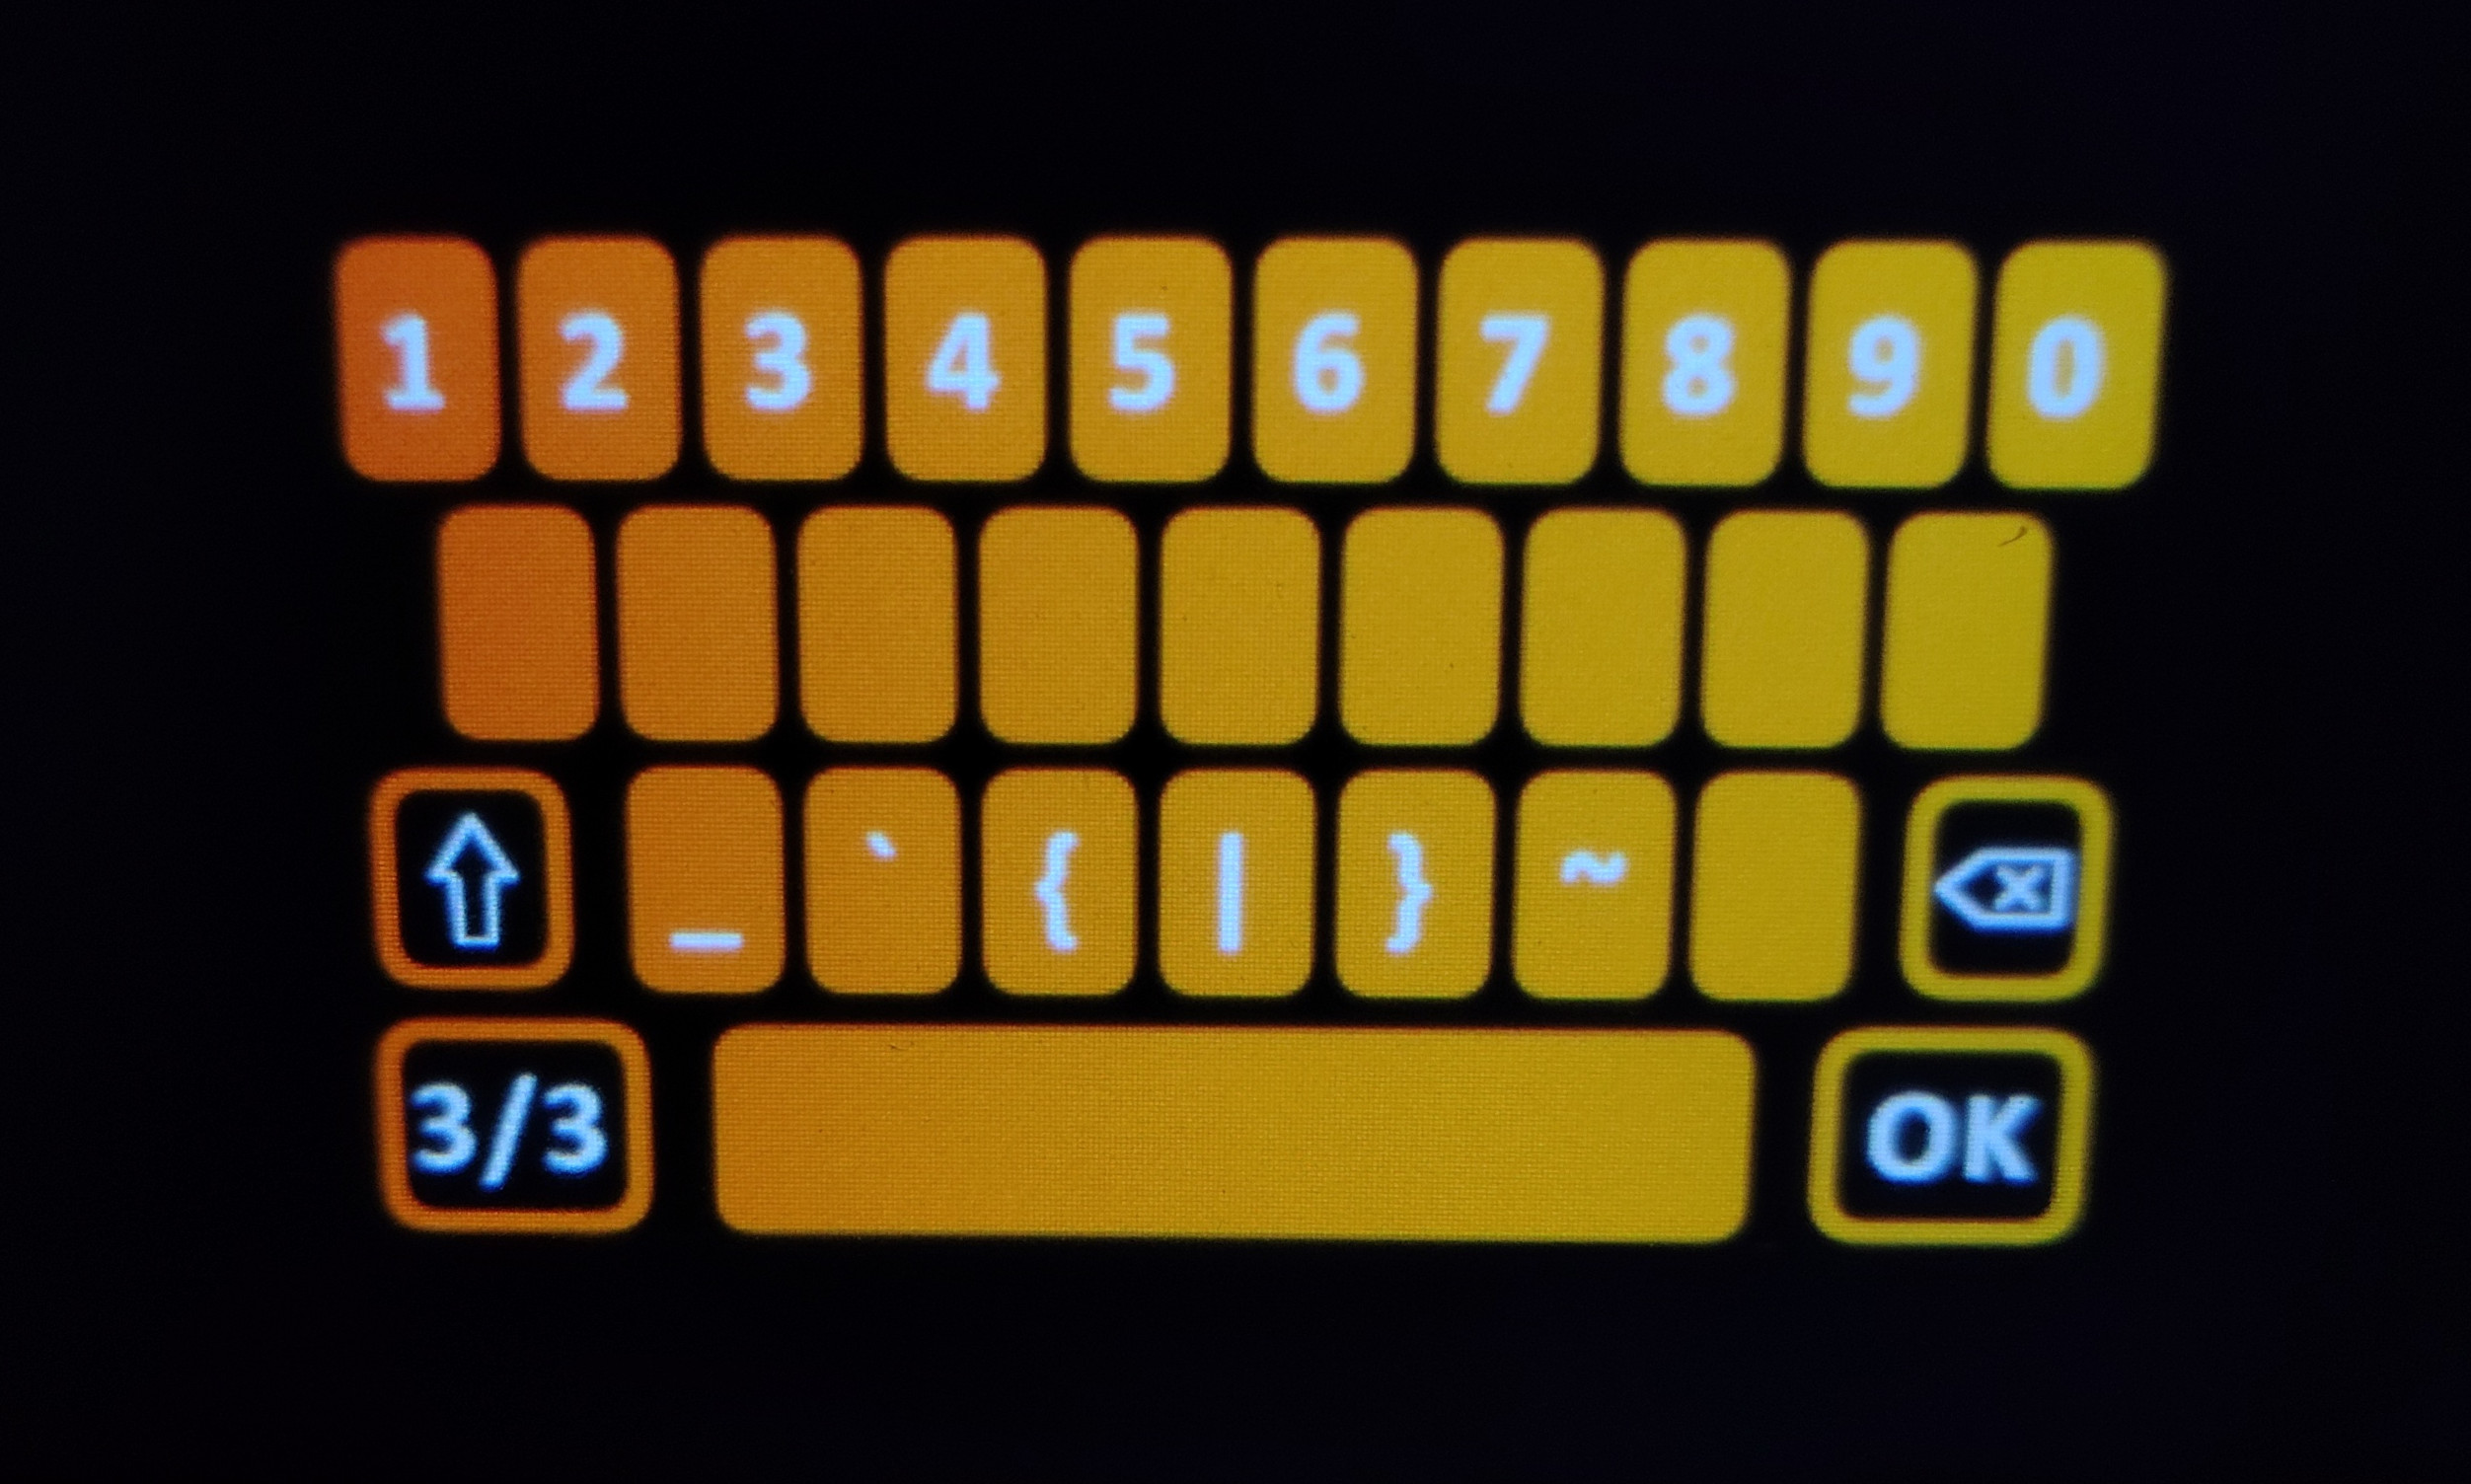
\includegraphics[width=\linewidth]{figures/keyboard_page3.jpg}
        \caption{Dritter Zeichensatz: Zahlen und mehr.}
    \end{subfigure}
\end{figure}

Der \textbf{zweite Zeichensatz} ist für Symbole gedacht und der \textbf{dritte} für Zahlen und weitere Sonderzeichen. Um zum dritten Zeichensatz zu gelangen, drücken Sie einfach die Taste \textbf{„2/3“} in der unteren linken Ecke der Tastatur. Im dritten Zeichensatz können Sie durch Drücken der Taste \textbf{„3/3“} wieder zum ersten Zeichensatz zurückkehren. Auf diesen beiden Seiten hat die Shift-Taste keine Funktion, da sie nicht benötigt wird.\\

Wenn Sie mit der Eingabe fertig sind, drücken Sie die Taste \textbf{OK}, um Ihre Eingabe zu bestätigen und zur vorherigen MQTT- oder WLAN-Einstellungsseite zurückzukehren, wo das bearbeitete Feld aktualisiert wird.

\subsection{Die reine Zahlentastatur}

In einigen Feldern, wie z.~B. der MQTT-Veröffentlichungsfrequenz, sind nur Zahlen erlaubt. In diesem Fall öffnet ToM+ eine reine Zahlentastaturseite, wie im Bild unten gezeigt.

\begin{figure}[H]
    \centering
    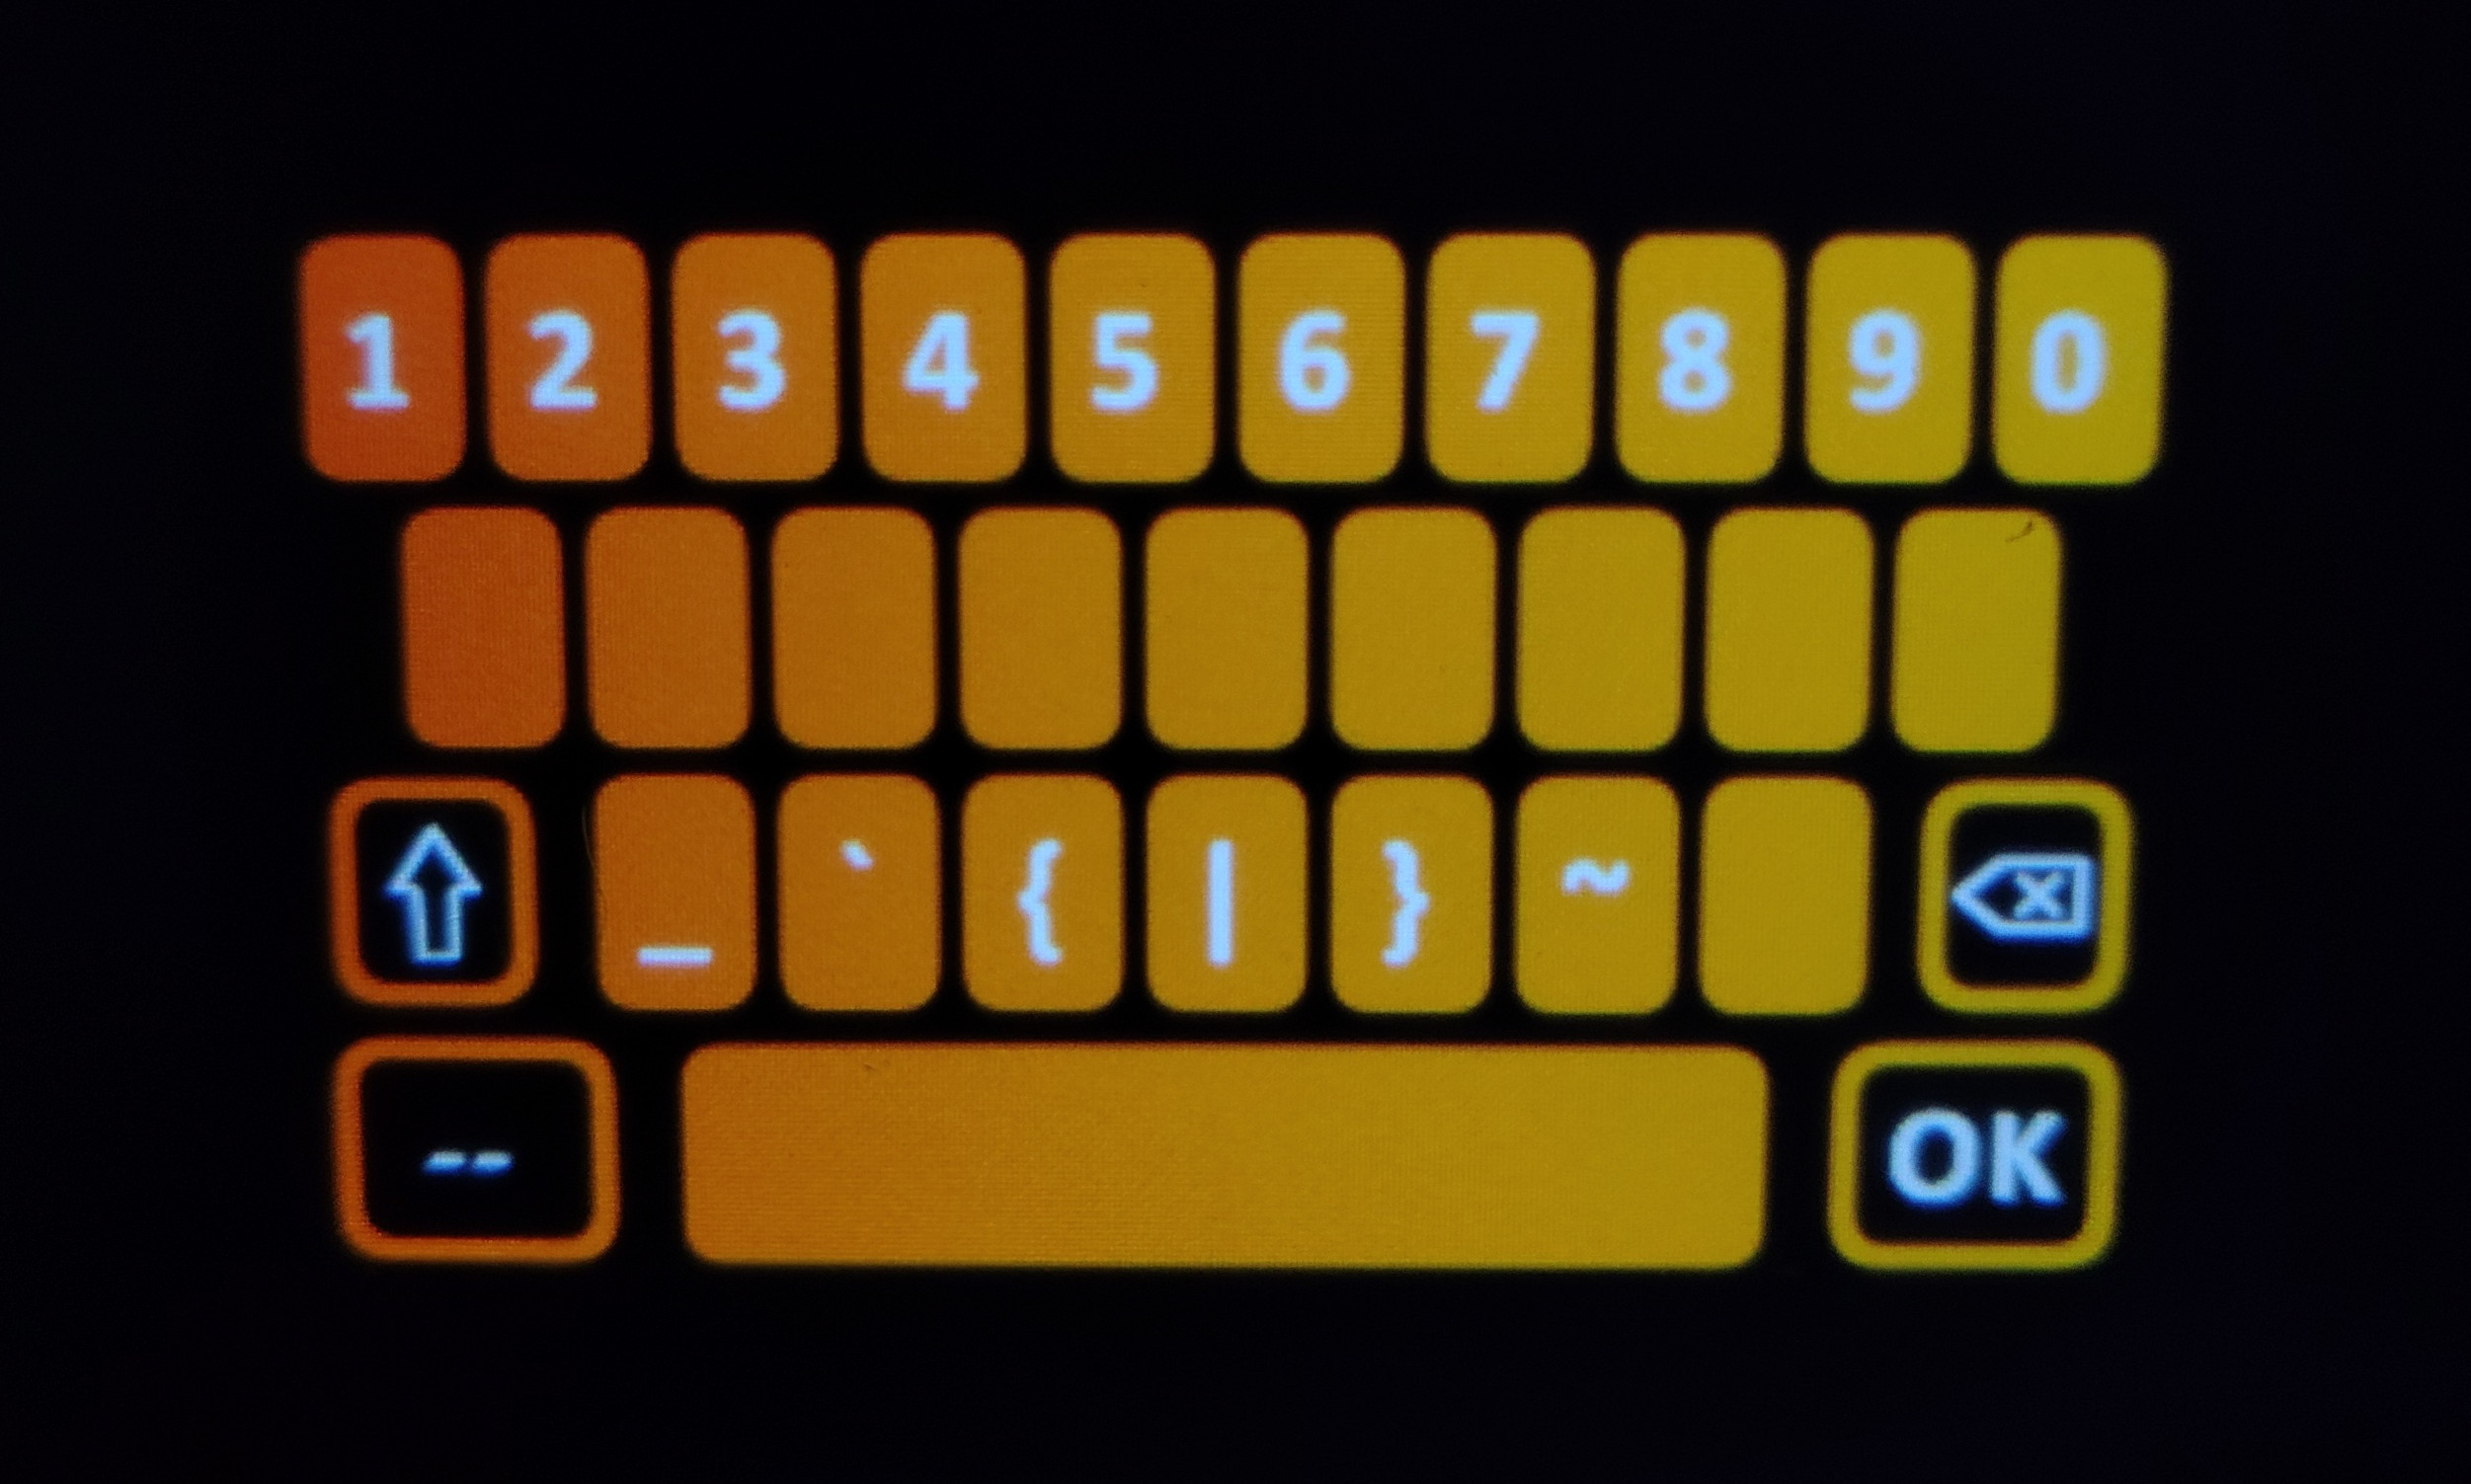
\includegraphics[width=0.8\textwidth]{figures/keyboard_num_only.jpg}
    \caption{Reine Zahlentastatur.}
\end{figure}

Wie Sie sehen können, ist das Layout dasselbe wie beim dritten Zeichensatz der vollständigen Tastatur, jedoch auf Zahlen und einige Sonderzeichen beschränkt. Sie werden auch bemerken, dass die Taste zum Wechseln des Zeichensatzes nicht verfügbar ist, da sie in diesem Fall nicht benötigt wird. Die Rücktaste steht weiterhin zum Löschen von Zeichen zur Verfügung, und die \textbf{OK-Taste} bestätigt Ihre Eingabe und führt zurück zur vorherigen Seite.



\section{Der Webserver}
\label{sec:web_server}

Der Webserver ist eine neue Funktion, die mit dem zweiten Firmware-Release eingeführt wurde. Er ermöglicht Ihnen den Fernzugriff auf Ihre ToM+-Einstellungen und -Daten von jedem Gerät mit einem Webbrowser, wie z.~B. Ihrem Smartphone, Tablet oder PC. Dies ist besonders nützlich für die Verwaltung von Standard- und \textbf{erweiterten Konfigurationen}, die auf dem ToM+-Display nicht verfügbar sind.

Zusätzlich können Sie den Webserver nutzen, um \textbf{WLAN und MQTT} viel einfacher einzurichten als nur über das ToM+-Display mit der Tastaturseite (Abschnitt~\ref{sec:keyboard_page}).\\

\begin{figure}[H]
    \centering
    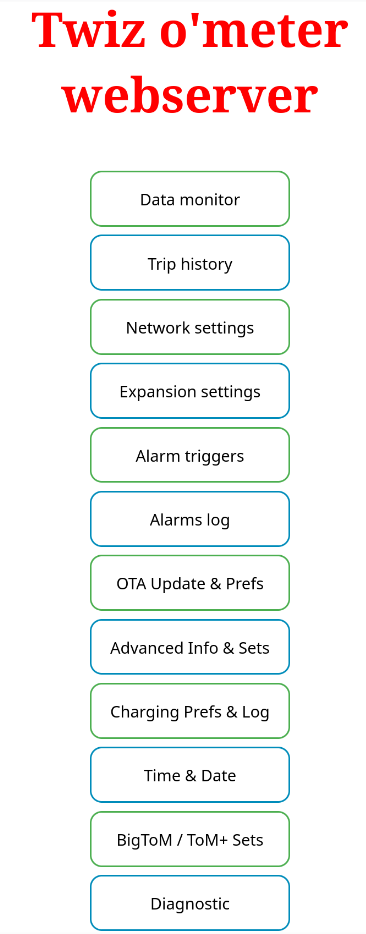
\includegraphics[width=0.46\textwidth]{figures/landing_page.png}
    \caption{Startseite des Webservers.}
\end{figure}


\subsection{Die Startseite}

Auf der oben gezeigten Startseite sehen Sie zwölf Schaltflächen, die Ihnen Zugriff auf verschiedene Seiten des Webservers geben. Hier gebe ich einen kurzen Überblick über die auf jeder Seite verfügbaren Funktionen, bevor diese in den folgenden Absätzen vertieft werden. In diesem Abschnitt dienen die Symbole nur als visuelle Hilfe:\\

\iconbox{icons/BatteryInfo2.png}
{Datenmonitor}{Hier können Sie Ihre Twizy-Daten in Echtzeit überwachen, organisiert in Tabellen genau wie auf den ToM+-Displayseiten (Abschnitt~\ref{sec:web_data_monitor}).}

\iconbox{icons/Street0Ok_v2.png}
{Fahrtenverlauf}{Hier können Sie die Daten jeder aufgezeichneten Fahrt (1 bis 5) und der letzten zwanzig Fahrten überprüfen, genau wie auf dem ToM+-Display (Abschnitt~\ref{sec:web_trip_history}).}

\iconbox{icons/Tray_WiFiOff.png}
{Netzwerkeinstellungen}{Hier können Sie Ihre WLAN-Verbindungsprofile und MQTT-Broker-Parameter einrichten, genau wie auf dem ToM+-Display (Abschnitt~\ref{sec:web_network_settings}).}

\iconbox{icons/Pin1.png}
{Erweiterungseinstellungen}{Hier können Sie die Pins des Erweiterungsanschlusses konfigurieren und das Verhalten für die rechte Scheibenwischerhebels-Taste wählen (Abschnitt~\ref{sec:web_expansion_settings}).}

\iconbox{icons/Alarm.PNG}
{Alarmauslöser}{Hier können Sie Alarme auf Basis von ToM+-Daten anzeigen oder einrichten und die Aktion auswählen, die beim Auslösen eines Alarms ausgeführt werden soll (Abschnitt~\ref{sec:web_alarm_triggers}).}

\iconbox{icons/Alarm.PNG}
{Alarmlogbuch}{Hier können Sie den Verlauf der letzten 21 Alarmauslösungen und deren Details, wie Datum und Uhrzeit, anzeigen und löschen (Abschnitt~\ref{sec:web_alarms_log}).}

\iconbox{icons/Swap.png}
{OTA-Update \& Einstellungen}{Hier können Sie die ToM+-Firmware über die OTA-Methode aktualisieren und Ihre ToM+-Einstellungen sichern/wiederherstellen (Abschnitt~\ref{sec:web_ota_update}).}

\iconbox{icons/Swap.png}
{Erweiterte Info \& Sets}{Hier können Sie erweiterte Informationen über Ihre Twizy-Batterie anzeigen und verschiedene Einstellungen konfigurieren (Abschnitt~\ref{sec:web_advanced_info}).}

\iconbox{icons/CEta.png}
{Ladeeinstellungen \& Log}{Hier können Sie Ladeeinstellungen festlegen, den Ladevorgang spontan abbrechen und die letzten 15 Lade-Protokolle anzeigen oder löschen (Abschnitt~\ref{sec:web_charging_prefs}).}

\iconbox{icons/Timer.PNG}
{Uhrzeit \& Datum}{Hier können Sie Uhrzeit und Datum Ihres ToM+ einstellen und die Zeitzone mithilfe von POSIX-TZ-Zeichenfolgen wählen oder mit WLAN synchronisieren (Abschnitt~\ref{sec:web_time_date}).}

\iconbox{icons/Kmh.png}
{BigToM / ToM+ Sets}{Hier können Sie einige Dashboard-Parameter konfigurieren, wie z.~B. die Skalierung des Leistungsbalkens oder das Einrichten eines Tempolimits (Abschnitt~\ref{sec:web_btom_tom_sets}).}

\iconbox{icons/Error.png}
{Diagnose}{Hier können Sie DTC/DF-Nummern und Beschreibungen Ihrer Twizy-Fehler anzeigen und die Protokolle bei Bedarf löschen (Abschnitt~\ref{sec:web_diagnostic}).}


\subsection{Auf den Webserver zugreifen}
\label{sec:web_server_access}

ToM+ ermöglicht es Ihnen, sich auf zwei Arten mit seiner Webserver-Seite zu verbinden, die beide in unterschiedlichen Situationen nützlich sind. Bevor wir beginnen, denken Sie daran, dass eine \textbf{IP-Adresse} im Grunde der numerische Name Ihres Geräts in einem Netzwerk ist (z.~B. \textit{192.168.1.100}).

\textbf{\textit{Für beide Methoden muss ToM+ mit einem Netzwerk verbunden sein.}}
Stellen Sie also sicher, dass Ihr ToM+ entweder ein wie in Abschnitt~\ref{sec:add_wifi_profile} erklärtes WLAN-Profil konfiguriert hat oder mit einem passwortfreien WLAN-Netzwerk verbunden ist. Um zu überprüfen, ob Ihr ToM+ verbunden ist, lesen Sie bitte Abschnitt~\ref{sec:check_wifi_connection}.\\

\textbf{Die erste und einfachste Einrichtung} besteht darin, den Hotspot Ihres Telefons ohne Passwort zu verwenden, sodass sich ToM+ verbindet, ohne ein WLAN-Profil konfigurieren zu müssen. Rufen Sie dann (immer noch auf Ihrem Telefon) Chrome oder Safari (oder einen beliebigen Webbrowser) auf und geben Sie die IP-Adresse von ToM+ ein (gezeigt in Abbildung~\ref{fig:wifi_bottom_line}).\\

\textbf{Die zweite Methode} funktioniert nur, wenn Sie sich in unmittelbarer Nähe des Twizy innerhalb der WLAN-Reichweite befinden. Sie können Ihr Telefon oder Ihren Laptop verwenden, um einen WLAN-Scan durchzuführen, und dann je nach Modell nach dem Netzwerk \textit{„ToM+ AP“}, \textit{„Twiz o'Meter AP“} oder \textit{„BigToM AP“} suchen. Als Nächstes sollten Sie sich mit dem \textbf{korrekten Passwort} mit diesem Netzwerk verbinden. Es ist anfänglich auf das Wort „pass“, gefolgt von der Seriennummer Ihres Geräts, eingestellt (z.~B. \textit{pass129777}). Die Seriennummer finden Sie auf der Einstellungsseite, wie in Abbildung~\ref{fig:settings_page} erklärt. Sie können es dann auf Wunsch ändern, aber es gibt kein Passwort-Wiederherstellungssystem (siehe Abschnitt~\ref{sec:web_change_password}). Sobald Sie mit dem ToM+ Access Point verbunden sind, geben Sie in einem beliebigen Browser seine statische IP-Adresse ein, die \textbf{192.188.1.188} lautet.


\subsection{Webserver-Passwort ändern}
\label{sec:web_change_password}

Um das Passwort für den Webserver zu ändern, rufen Sie auf dem Display die WLAN-Einstellungsseite auf (Abschnitt~\ref{sec:wifi_settings}) und tippen Sie auf das Feld \textbf{„KEY 4“}. Dadurch wird die Tastaturseite geöffnet (Abschnitt~\ref{sec:keyboard_page}), auf der Sie Ihr neues Passwort eingeben können. Dieses Passwort wird dann sowohl als Access-Point-Passwort als auch für das vierte WLAN-Verbindungsprofil verwendet.


\subsection{Datenmonitor-Seite}
\label{sec:web_data_monitor}

Wie in der Einleitung erwähnt, listet diese Seite alle verfügbaren ToM+-Daten auf, geordnet in sieben verschiedenen Tabellen, von denen jede nur die in ihrer Kopfzeile angegebenen Daten enthält. Die Datenverteilung entspricht der in Abschnitt~\ref{sec:icon_list} verwendeten und kann nicht geändert werden.

Diese Werte werden \textbf{alle 10 Sekunden aktualisiert} und sind mit ihrer Maßeinheit gekoppelt. Machen Sie sich keine Sorgen um Ihre Privatsphäre, da Ihre Daten verpackt in einer speziellen Paketstruktur übertragen werden, die schwer abzuhören oder zu knacken ist. Darüber hinaus nutzt der Webserver keine externen Dienste oder MQTT für die Überwachung, sodass Ihre Daten privat und sicher bleiben. Die Seite wird vollständig direkt von der Blackbox generiert und unterliegt keiner weiteren Verarbeitung.

\begin{figure}[H]
    \centering
    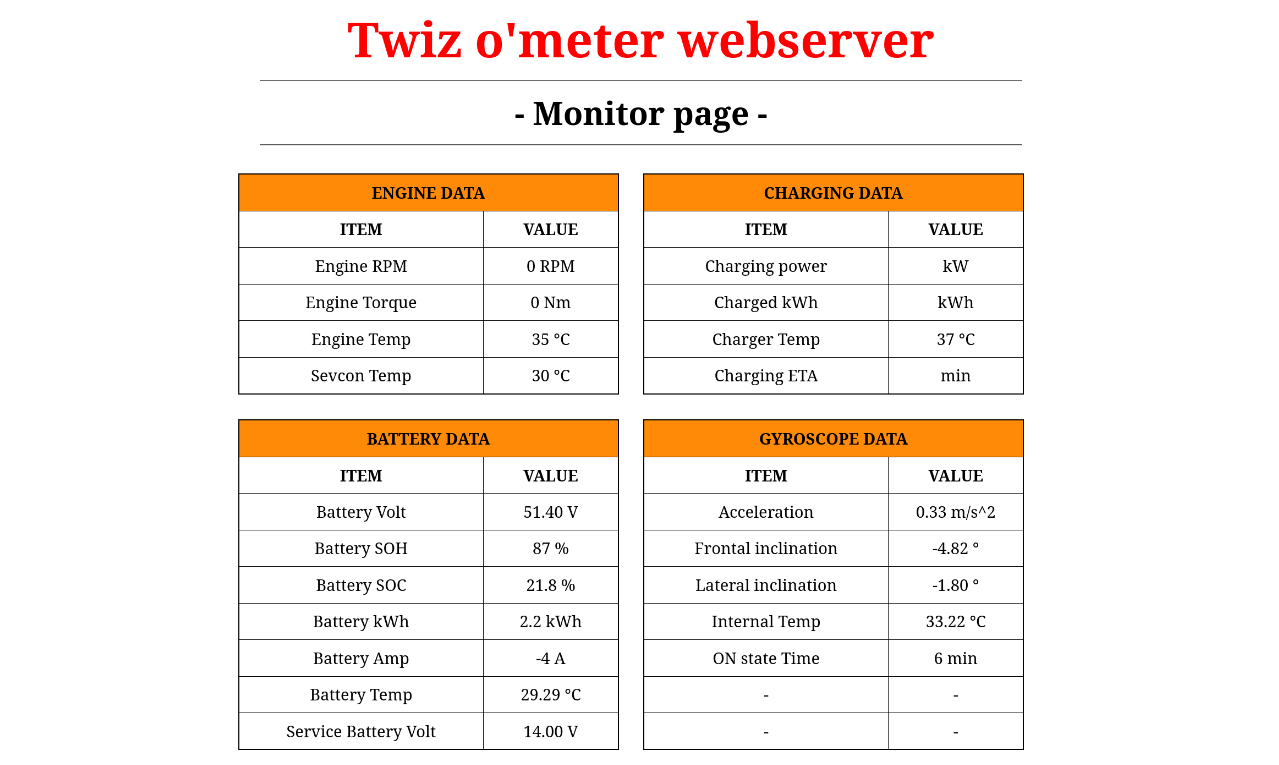
\includegraphics[width=1\textwidth]{figures/monitor_page1.png}
    \caption{Datenmonitor-Seite --- obere Tabellen.}
\end{figure}

Im zweiten Teil der Seite befinden sich die letzten drei Tabellen, die Dashboard-Daten und Daten des Erweiterungsanschlusses enthalten; die letzte enthält alle Spannungen und Temperaturen der Batterie-Infos. Drücken Sie die vom roten Pfeil angezeigte grüne Taste \textbf{„HOME“}, um zur Startseite zurückzukehren.

\begin{figure}[H]
    \centering
    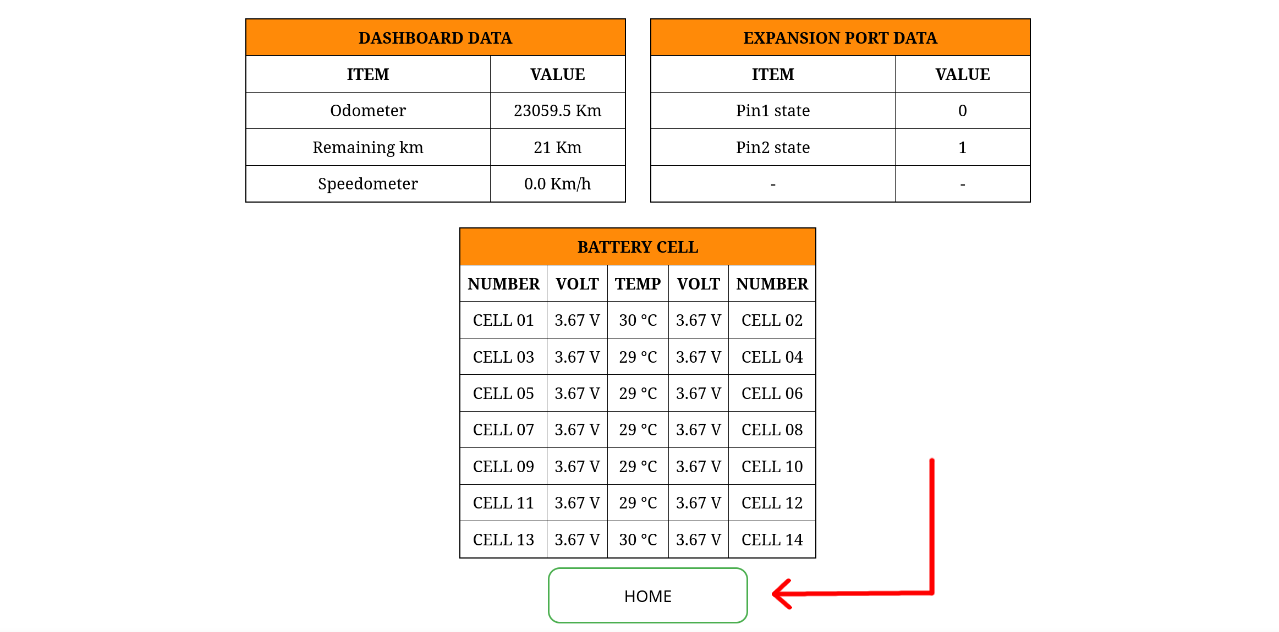
\includegraphics[width=1\textwidth]{figures/monitor_page2.png}
    \caption{Datenmonitor-Seite --- untere Tabellen.}
\end{figure}

\clearpage

\subsection{Fahrtenverlauf-Seite}
\label{sec:web_trip_history}

Diese enthält die Werte der zuvor in Abschnitt~\ref{sec:trip_page} besprochenen Fahrtenseite. Sie kann bis zu 5 verschiedene Datensätze speichern, und selbst wenn die auf dem Display angezeigten Daten begrenzt sind, werden sie auf der Webserver-Seite alle angezeigt. Die erste Tabelle zeigt Fahrten, jeweils organisiert in fünf Zeilen, und die Kopfzeilen jedes Datensatzes sind in Abschnitt~\ref{sec:icon_list} aufgeführt.

\begin{figure}[H]
    \centering
    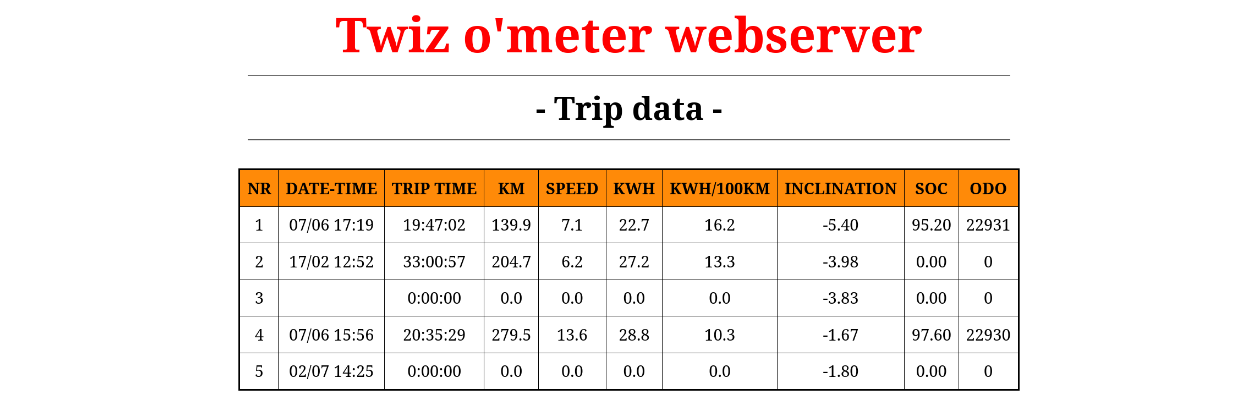
\includegraphics[width=1\textwidth]{figures/trip_page1.png}
    \caption{Fahrtenverlauf-Seite --- Fahrtendaten.}
\end{figure}

Die zweite Tabelle zeigt die letzten zwanzig Fahrten (ab der aktuellsten) mit denselben Kopfzeilen wie die erste Tabelle. Sie können zur Startseite zurückkehren, indem Sie die grüne Taste \textbf{„HOME“} direkt unter der zweiten Tabelle drücken.

\begin{figure}[H]
    \centering
    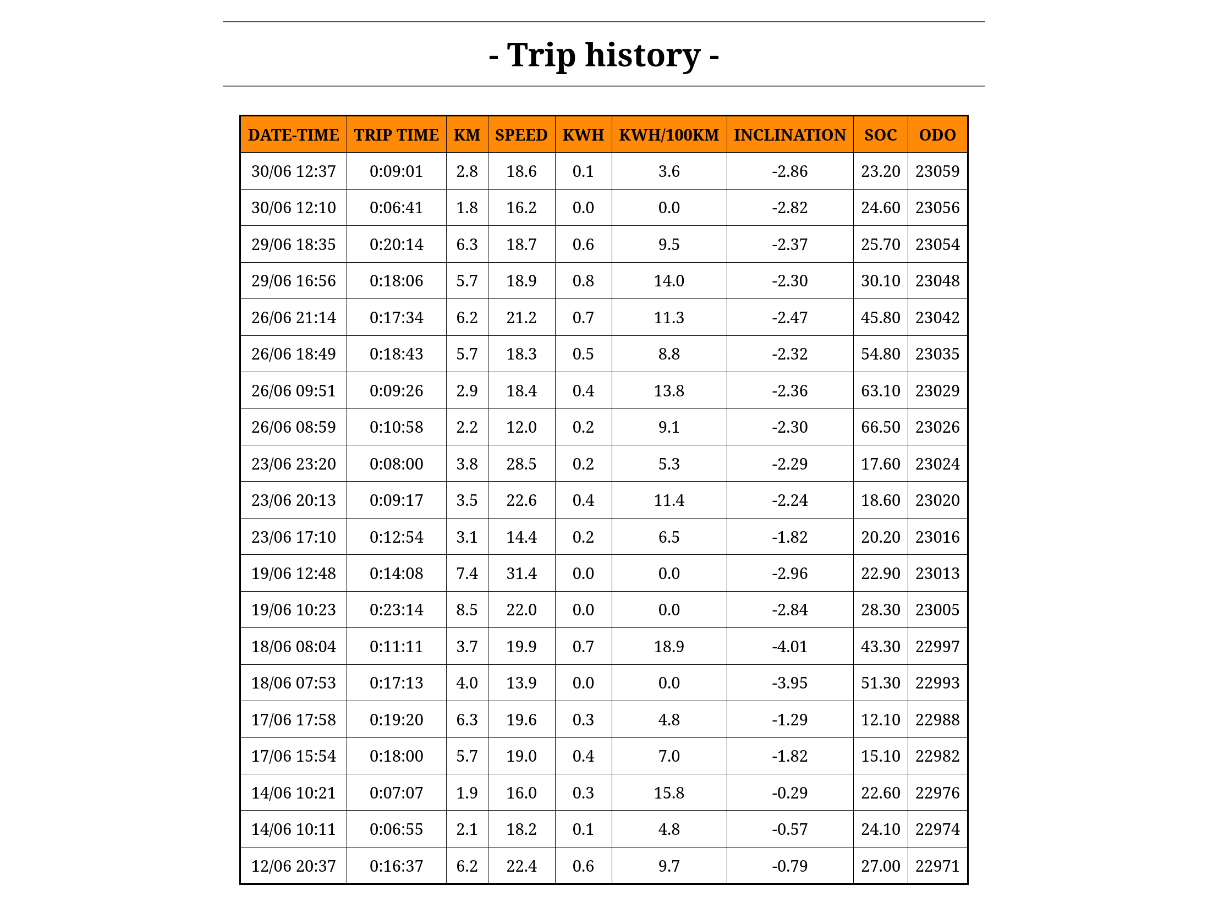
\includegraphics[width=1\textwidth]{figures/trip_page2.png}
    \caption{Fahrtenverlauf-Seite --- Fahrtenhistorie.}
\end{figure}


\subsection{Netzwerkeinstellungsseite}
\label{sec:web_network_settings}

Auf dieser Seite können Sie WLAN-Profile und den MQTT-Broker konfigurieren, ohne sich mit der Tastatur des ToM+-Displays abmühen zu müssen. Die Seite ist in zwei Haupttabellen unterteilt, eine für WLAN (Abschnitt~\ref{sec:wifi_settings}) und die andere für MQTT-Einstellungen (Abschnitt~\ref{sec:MQTT}).\\

Wie Sie im Bild sehen können, enthält die erste alle vier Profile, die zuvor auf dem ToM+ eingestellt wurden, oder, falls nicht, deren Standardwerte. Das Gleiche gilt für Passwörter, die erst sichtbar sind, wenn Sie die Schaltfläche „O“ neben dem Passwort drücken, das Sie sehen möchten. Erneutes Drücken blendet das Passwort wieder aus. Hier können Sie auch das WLAN-Passwort für den Access Point ändern (Abschnitt~\ref{sec:web_change_password}).

\begin{figure}[H]
    \centering
    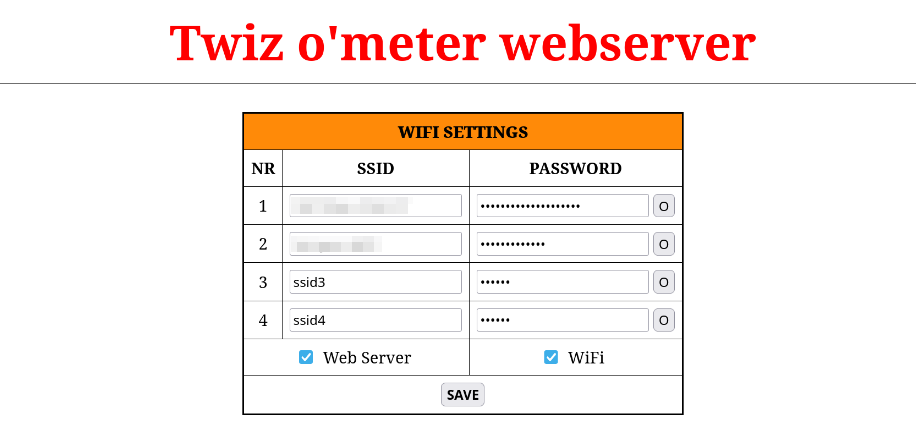
\includegraphics[width=1\textwidth]{figures/wifi_page1.png}
    \caption{Netzwerkeinstellungsseite --- WLAN-Tabelle.}
\end{figure}

Die beiden Kontrollkästchen erfüllen dieselben Funktionen wie die beiden Schieberegler auf der WLAN-Einstellungsseite des ToM+. Wofür diese verwendet werden, erfahren Sie in Abschnitt~\ref{sec:enable_disable_wifi}. Nach jeder Änderung drücken Sie die Schaltfläche \textbf{„SAVE“}, um Ihre Änderungen zu speichern; andernfalls gehen sie beim Verlassen der Seite verloren.

\begin{figure}[H]
    \centering
    
\includegraphics[width=1\textwidth]{figures/wifi_page3.png}
    \caption{Netzwerkeinstellungsseite --- WLAN-Statustabelle.}
\end{figure}

Wenn Ihr ToM+ mit einem Netzwerk verbunden ist, erscheint unterhalb der eben besprochenen Tabelle eine kleine Tabelle, deren Zeilen drei Hauptinformationen enthalten: die SSID, die IP-Adresse des ToM+ und die MAC-Adresse. Diese Daten finden Sie auch auf dem ToM+-Display auf der WLAN-Einstellungsseite, wie zuvor in Abbildung~\ref{fig:wifi_bottom_line} gezeigt.\\

Die zweite Haupttabelle enthält hingegen die Einstellungen des MQTT-Brokers, wie sie zuvor auf dem ToM+-Display konfiguriert wurden, oder, falls nicht, Standardwerte (\textit{z.~B. „broker.address“}). Sie können diese bequem manuell auf dieser Webserver-Seite ändern, was viel komfortabler ist als die Verwendung der Tastatur des ToM+-Displays. Schauen Sie sich im Bild unten an, wie diese Tabelle nach der Konfiguration aussehen kann.

\begin{figure}[H]
    \centering
    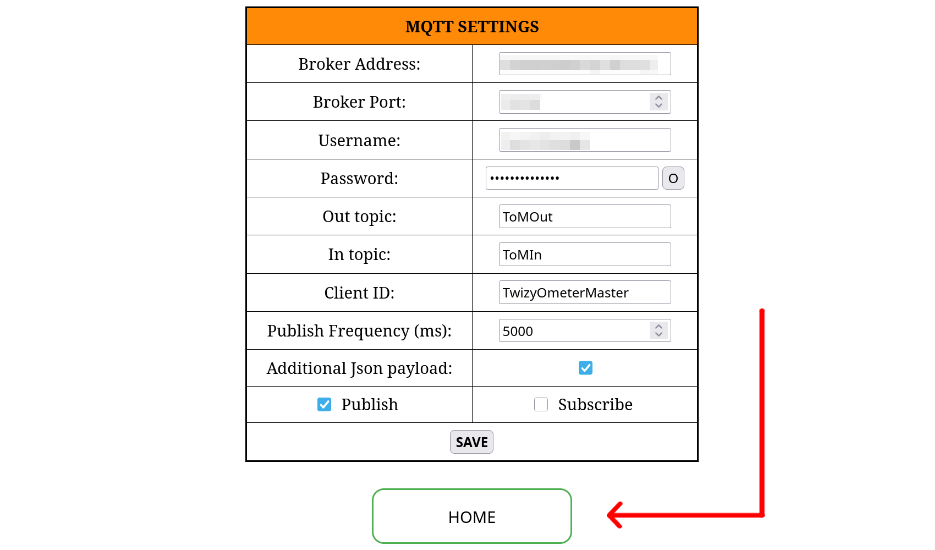
\includegraphics[width=1\textwidth]{figures/wifi_page2.png}
    \caption{Netzwerkeinstellungsseite --- MQTT-Tabelle.}
\end{figure}

Die beiden Kontrollkästchen erfüllen dieselben Funktionen wie die beiden Schieberegler auf der MQTT-Einstellungsseite von ToM+. Wofür sie verwendet werden, erfahren Sie in Abschnitt~\ref{sec:enable_disable_mqtt}. Wenn Ihr ToM+ mit dem MQTT-Broker verbunden ist, enthält die Tabellenkopfzeile den Text \textbf{„(CONNECTED!)“}.\\

Nach jeder Änderung drücken Sie die Schaltfläche \textbf{„SAVE“}, um Ihre Änderungen zu speichern; andernfalls gehen sie beim Verlassen der Seite verloren. Am Ende dieser Seite befindet sich, im Bild durch einen roten Pfeil gekennzeichnet, die grüne Schaltfläche \textbf{„HOME“}, um zur Startseite zurückzukehren.


\subsection{Erweiterungseinstellungsseite}
\label{sec:web_expansion_settings}

Diese Seite enthält die Konfiguration für PIN1 und PIN2 des Erweiterungsanschlusses sowie die Konfiguration für die rechte Scheibenwischerhebels-Taste. Sie kann sehr nützlich sein, wenn Sie Dinge anpassen und Ihrem ToM+ eine persönliche Note verleihen möchten. Die Pin-Belegung des Erweiterungsanschlusses ist in Abbildung~\ref{fig:expansion_pinout} dargestellt. Da es sich um allgemeine Ein-/Ausgabe-Pins handelt, können Sie den Modus für jeden einzelnen Pin je nach Bedarf wählen.\\

Wenn Sie den Modus \textbf{„INPUT“} wählen, lauscht diese Leitung auf das im nächsten Feld angegebene Signal. Dies kann beim Einrichten eines sehr spezifischen Alarms sehr nützlich sein, aber wir werden dies später besprechen. Wenn Sie hingegen den Modus \textbf{„OUTPUT“} wählen, überträgt ToM+ das im nächsten Feld angegebene Signal, das HIGH (5V) oder LOW (0V) sein kann, wenn ein Alarm ausgelöst wird. Wie bereits erwähnt, wird dies in Abschnitt~\ref{sec:web_alarm_triggers} vertieft.\\

Seit den neuesten Firmware-Releases wurden den Erweiterungs-PINs neue Modi neben INPUT und OUTPUT hinzugefügt. Schauen wir uns diese genauer an:\\

\begin{itemize}
    \item \textbf{IR CONTROLLER}: Dieser Modus ermöglicht die Steuerung von ToM+ über eine Infrarot-Fernbedienung.
    \item \textbf{KEY+ CONTROLLER}: Dieser Modus ermöglicht die Steuerung Ihres ToM+ über eine Infrarot-Drehfernbedienung. Für diese beiden ersten Modi erscheint eine zusätzliche Konfigurationstabelle.
    \item \textbf{SERIAL TX}: Ermöglicht die Konfiguration einer seriellen TX-Leitung (noch nicht implementiert).
    \item \textbf{SERIAL RX}: Ermöglicht die Konfiguration einer seriellen RX-Leitung (noch nicht implementiert).
    \item \textbf{CTRL BUTTON}: Dieser Modus ermöglicht es Ihnen, die rechte Scheibenwischerhebels-Taste als Steuertaste für Ihre ToM+-Gesten zu verwenden.
\end{itemize}

\subsubsection{Standard-OUTPUT-Modus}

Sowohl im \textbf{„OUTPUT“}- als auch im \textbf{„INPUT“}-Modus müssen Sie zuerst zwischen \textit{„Active High“} und \textit{„Active Low“} wählen. Wenn ein Alarm auslöst, wird ein LOW/HIGH-Signal an den PIN gesendet, der als Alarmausgang ausgewählt wurde (entweder PIN1 oder PIN2).

Wenn Sie \textit{„Active High“} wählen, ist das gesendete Signal HIGH (5V) und wird normalerweise auf LOW (0V) gehalten.

Wenn Sie \textit{„Active Low“} wählen, ist das gesendete Signal LOW (0V) und wird normalerweise auf HIGH (5V) gehalten.

\begin{figure}[H]
    \centering
    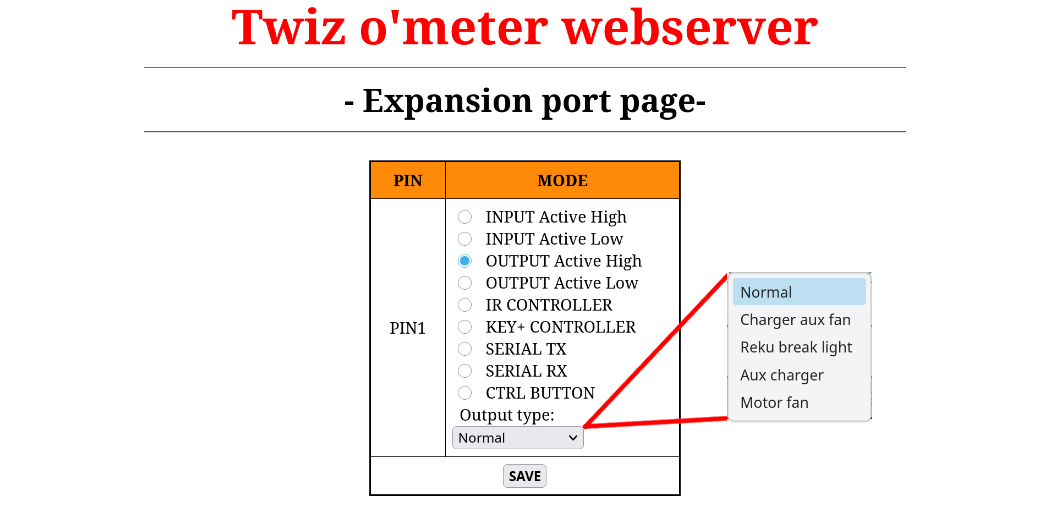
\includegraphics[width=1\textwidth]{figures/expansion_page1.png}
    \caption{Erweiterungseinstellungsseite --- PIN1-Tabelle.}
\end{figure}

Wie Sie im Bild unten sehen können, können Sie bei Auswahl des Modus \textbf{„OUTPUT“} auch den \textit{„Output Type“} wählen. Dies ist nützlich, wenn Sie ein sehr spezifisches Ausgabegerät haben, das eine zusätzliche Verwaltung erfordert, die nicht auf das Standard-HIGH/LOW-Signal beschränkt ist. Um dies zu erreichen, können Sie aus einer Liste bereits verwalteter Ausgabegeräte wählen, die im Bild oben hervorgehoben sind.\\

Nach jeder Änderung drücken Sie die Schaltfläche \textbf{„SAVE“}, um Ihre Änderungen zu speichern; andernfalls gehen sie beim Verlassen der Seite verloren. Wenn Sie eine Idee für ein neues Ausgabegerät haben, das für die Community nützlich sein könnte, können Sie mich gerne kontaktieren.\\

\begin{itemize}
    \item \textit{„Normal“}: Dies ist der Standard-OUTPUT-Modus, beschränkt auf HIGH/LOW-Signale.
    \item \textit{„Charger auxilliary fan“}: Damit können Sie einen Zusatzlüfter steuern. Sie müssen einen Alarm für die Ladegerättemperatur mit einem Schwellenwert einrichten. Wenn dieser beim Laden ausgelöst wird, beginnt der Lüfter mit der Kühlung des Ladegeräts und stoppt erst, wenn die Temperatur unter den ausgewählten Schwellenwert mit einer festen Hysterese fällt (falls erforderlich auch nach dem Ende des Ladevorgangs).
    \item \textit{„Reku break light“}: Damit können Sie eine Relaisplatine anschließen, die das Bremslicht steuert, um es im Rekuperationsmodus einzuschalten. Dies ist besonders nützlich, wenn Ihr Twizy getunt ist, um die Rekuperationsleistung zu erhöhen.
    \item \textit{„Auxilliary charger“}: Damit können Sie ein Zusatzladegerät mit einem Alarm für SOC oder Batteriespannung steuern. Es ermöglicht den Anschluss einer Relaisplatine, die bei Bedarf ein Zusatzladegerät aktiviert oder deaktiviert. Es schaltet sich nur im Lademodus mit einer kleinen festen Verzögerung ein.
    \item \textit{„Motor fan“}: Damit können Sie einen Motorlüfter mit einem Alarm für die Motortemperatur steuern. Es funktioniert genauso wie der Ladegerätlüfter mit dem Unterschied, dass dies nur während der Fahrt funktioniert.
\end{itemize}

\subsubsection{Standard-INPUT-Modus}

Wie Sie im Bild unten sehen können, erscheinen bei Auswahl des Modus \textbf{„INPUT“} keine zusätzlichen Tabellen. Dieser Modus stützt sich stark auf die Alarmkonfiguration und Auslöser; lesen Sie daher bitte Abschnitt~\ref{sec:web_alarm_triggers}. Wir haben in der zweiten Tabelle den Modus \textbf{„INPUT“} gewählt, der genauso funktioniert, aber für PIN2 des Erweiterungsanschlusses vorgesehen ist.

Nach jeder Änderung drücken Sie die Schaltfläche \textbf{„SAVE“}, um Ihre Änderungen zu speichern; andernfalls gehen sie beim Verlassen der Seite verloren.

\begin{figure}[H]
    \centering
    
\includegraphics[width=1\textwidth]{figures/expansion_page3.png}
    \caption{Erweiterungseinstellungsseite --- PIN2-Tabelle.}
\end{figure}

\subsubsection{IR CONTROLLER-Modus}

Zunächst benötigen Sie einen IR-Empfänger (entweder einen Sensor oder ein Modul wie das im ersten Bild), der an einen der PINs der Erweiterungsplatine angeschlossen wird. Dieser Modus ist für die Verwendung mit einer allgemeinen IR-Fernbedienung vorgesehen, aber ich persönlich empfehle die im zweiten Bild unten gezeigte, die speziell für die Anbringung am Lenkrad entwickelt wurde.

\begin{figure}[ht]
    \centering

    \begin{subfigure}[t]{0.48\textwidth}
        \centering
        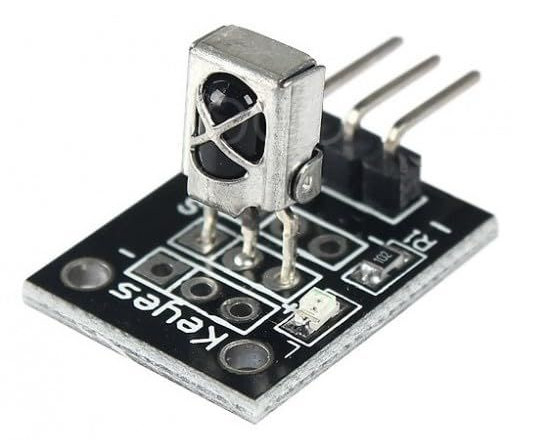
\includegraphics[width=\linewidth]{figures/ir_receiver.jpg}
        \caption{IR-Empfängermodul.}
    \end{subfigure}
    \hfill
    \begin{subfigure}[t]{0.48\textwidth}
        \centering
        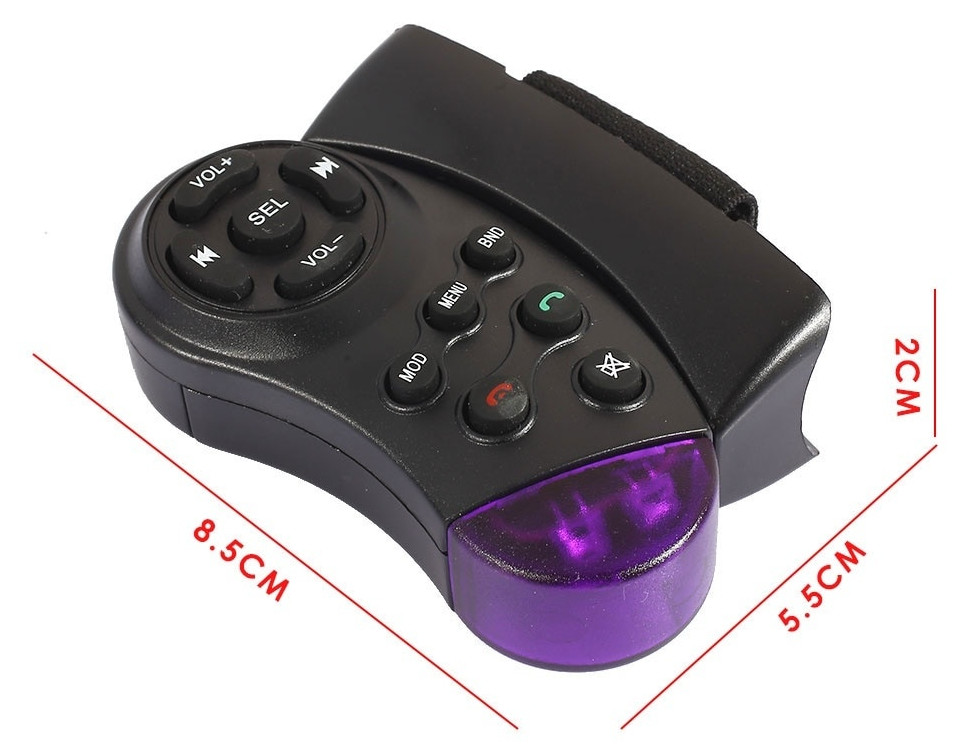
\includegraphics[width=\linewidth]{figures/ir_controller_photo.jpg}
        \caption{IR-Fernbedienung für das Lenkrad.}
    \end{subfigure}
\end{figure}

Wenn Sie den Modus \textbf{„IR CONTROLLER“} für die Tabelle von PIN1 oder PIN2 wählen, denken Sie daran, die Schaltfläche \textbf{„SAVE“} zu drücken, um Ihre Änderungen zu speichern. Sobald Sie gespeichert haben, wird die Seite neu geladen und unten erscheint eine zusätzliche Tabelle, die Sie im folgenden Bild sehen können.

\begin{figure}[H]
    \centering
    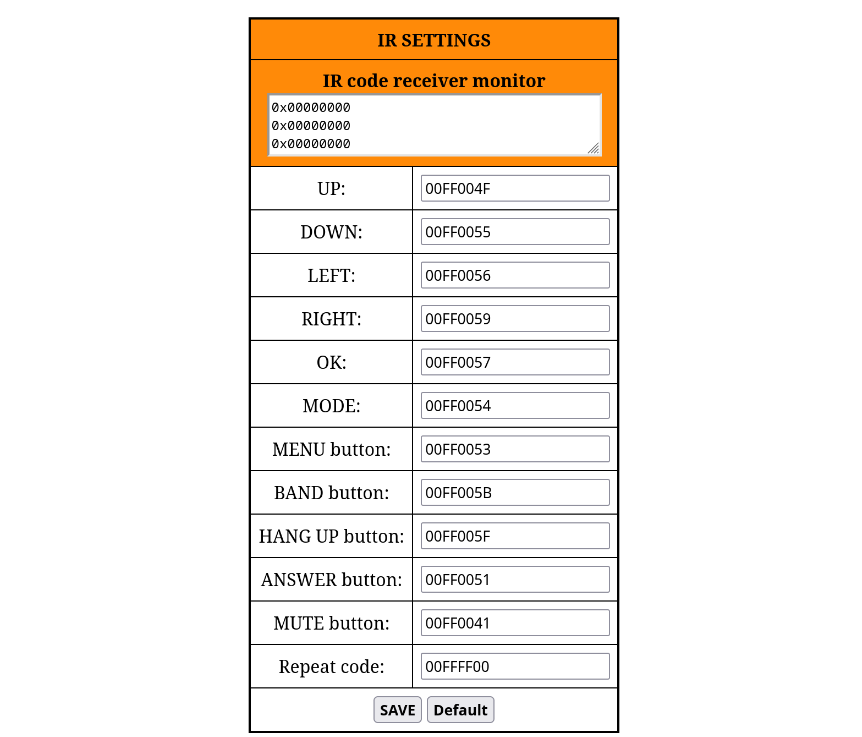
\includegraphics[width=0.8\textwidth]{figures/ir_settings.png}
    \caption{Erweiterungseinstellungsseite --- IR-Einstellungstabelle.}
\end{figure}

Diese Tabelle hilft Ihnen, jede Taste der IR-Fernbedienung mit dem entsprechenden IR-Code zu koppeln. Im oberen Teil der Tabelle befindet sich ein kleiner Textbereich, den Sie als \textbf{IR-Code-Empfangsmonitor} verwenden können, um IR-Codes Ihrer Fernbedienung nach dem Anschließen des IR-Empfängers in Echtzeit zu testen.\\

Damit können Sie die anderen Felder entsprechend ausfüllen. Das letzte ist besonders wichtig und ist im Grunde der Code, den die Fernbedienung sendet, wenn Sie eine Taste gedrückt halten. Vergessen Sie danach nicht, die Schaltfläche \textbf{„SAVE“} zu drücken, um Ihre Änderungen zu speichern; andernfalls gehen sie beim Verlassen der Seite verloren. Schließlich befindet sich daneben eine nützliche Schaltfläche \textbf{„Default“}, um Ihre Änderungen bei Bedarf einfach zurückzusetzen.

\subsubsection{KEY+ CONTROLLER-Modus}

Dieser Modus ist dem eben besprochenen sehr ähnlich, ist jedoch für die Verwendung mit einem anderen Controller-Typ vorgesehen (dem im Bild unten). Es handelt sich um einen drahtlosen Bluetooth-Drehcontroller für Autoradios, der je nachdem, wie schnell/langsam Sie den äußeren Ring drehen, verschiedene Aktionen ausführt. Und natürlich hat er auch noch einige Tasten im inneren Teil.\\

\begin{figure}[H]
    \centering
    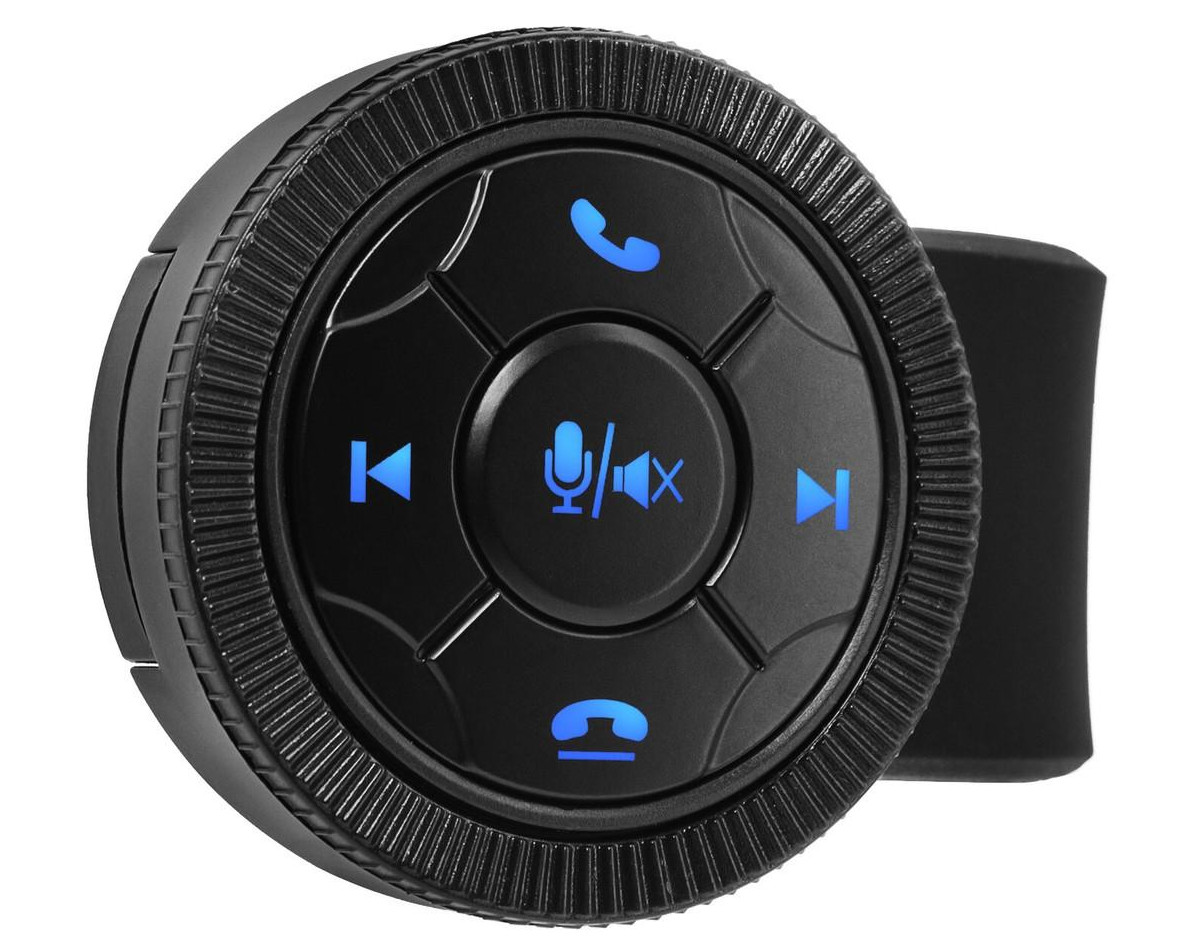
\includegraphics[width=0.4\textwidth]{figures/keyp_controller.jpg}
    \caption{Drahtloser Bluetooth-Drehcontroller.}
\end{figure}

Wenn Sie den Modus \textbf{„KEY+ CONTROLLER“} für die Tabelle von PIN1 oder PIN2 wählen, denken Sie daran, die Schaltfläche \textbf{„SAVE“} zu drücken, um Ihre Änderungen zu speichern. Sobald Sie gespeichert haben, wird die Seite neu geladen und unten erscheint eine zusätzliche Tabelle, die Sie im Bild unten sehen können.

\begin{figure}[H]
    \centering
    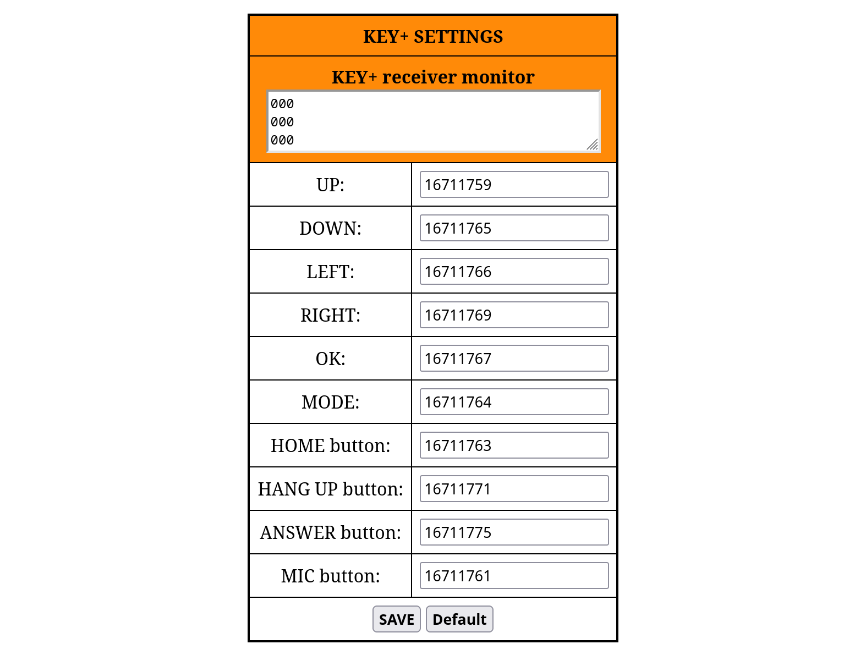
\includegraphics[width=0.8\textwidth]{figures/keyp_settings.png}
    \caption{Erweiterungseinstellungsseite --- KEY+-Einstellungstabelle.}
\end{figure}

Dies funktioniert genauso wie die IR-Einstellungstabelle. Der Hauptunterschied besteht darin, was ToM+ vom Erweiterungsanschluss liest, was kein IR-Code mehr ist, sondern eine Spannung.

Im Bild oben sind die Standardwerte dargestellt, die von \textit{0} bis \textit{3,3V} reichen und ohne Dezimalpunkt geschrieben werden. Beispiel: \textit{018} bedeutet \textit{0,18V} und \textit{157} bedeutet \textit{1,57V} usw. ToM+ hat eine Toleranz von \textit{0,05V} auf die Eingabewerte, um Spannungsschwankungen zu vermeiden.\\

Vergessen Sie danach nicht, die Schaltfläche \textbf{„SAVE“} zu drücken, um Ihre Änderungen zu speichern; andernfalls gehen sie beim Verlassen der Seite verloren. Schließlich befindet sich daneben eine nützliche Schaltfläche \textbf{„Default“}, um Ihre Änderungen bei Bedarf einfach zurückzusetzen.

\subsubsection{CTRL BUTTON-Modus}
\label{sec:web_wiper_stalk}

Diese letzte Tabelle enthält die Konfiguration, die erforderlich ist, damit die mitgelieferte rechte \textbf{Scheibenwischerhebels-Taste} (Abbildung~\ref{fig:wiper_stalk_button}) funktioniert. Sie können diese Taste verwenden, um durch die gesamte ToM+-Benutzeroberfläche zu navigieren, ohne den Touchscreen zu benutzen, und zwar mit diesen drei Haupt-\textbf{Aktionen}: \textit{„Browse items“}, \textit{„Change page“}, \textit{„Select-deselect“}. Um dies zu erreichen, gibt es drei Arten von \textbf{Tastendrücken}: \textit{„Short“}, \textit{„Medium“}, \textit{„Long“}.\\

\begin{figure}[H]
    \centering
    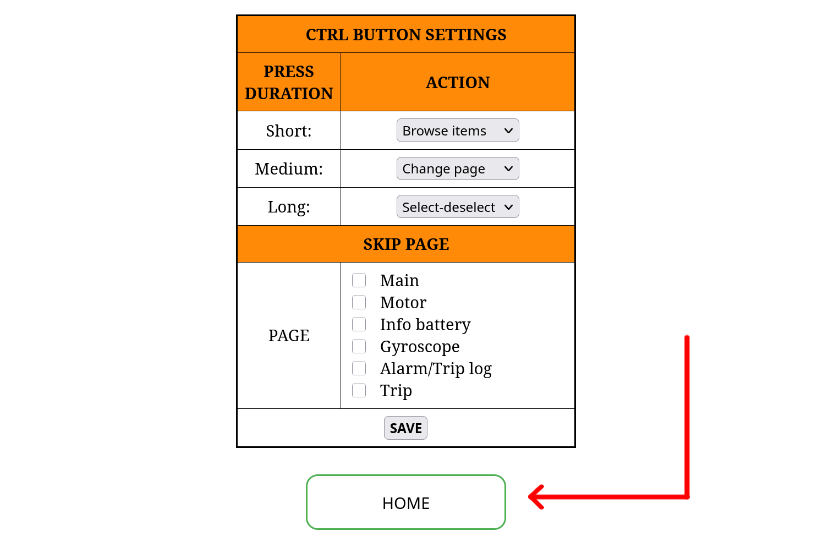
\includegraphics[width=1\textwidth]{figures/expansion_page2.png}
    \caption{Erweiterungseinstellungsseite --- Tabelle für Scheibenwischerhebels-Taste.}
\end{figure}

Im ersten Teil dieser Tabelle können Sie diese Aktionen mit den von Ihnen bevorzugten Gesten neu anordnen.\\

\begin{itemize}
    \item \textit{„Browse items“}: Bewegt eine kleine weiße Markierung neben die aktuell ausgewählten Daten.
    \item \textit{„Change page“}: Ermöglicht das Durchblättern der in der Rotation vorhandenen Seiten.
    \item \textit{„Select-deselect“}: Simuliert das Tippen auf die ausgewählten Daten (z.~B. Wechsel von Hintergrund zu Vordergrund).\\
\end{itemize}

Im zweiten Teil der Tabelle können Sie die \textbf{Seiten auswählen, die Sie überspringen möchten}, wenn Sie mit der Geste \textit{„Change page“} durch die verfügbaren Seiten blättern. Wenn ich beispielsweise die Batterie-Info-Seite beim Blättern mit der Taste nicht überwachen möchte, deaktiviere ich sie einfach, und sie wird aus der Rotation entfernt.\\

Nach jeder Änderung drücken Sie die Schaltfläche \textbf{„SAVE“}, um Ihre Änderungen zu speichern; andernfalls gehen sie beim Verlassen der Seite verloren. Am Ende dieser Seite befindet sich, im Bild durch einen roten Pfeil gekennzeichnet, die grüne Schaltfläche \textbf{„HOME“}, um zur Startseite zurückzukehren.

\clearpage

\subsection{Alarmauslöser-Seite}
\label{sec:web_alarm_triggers}

Wenn auf ToM+ etwas passiert und Sie darüber benachrichtigt werden möchten, können Sie auf dieser Seite auswählen, wie und wann Sie benachrichtigt werden möchten. Sie können bis zu \textbf{zehn Alarme} gleichzeitig laufen lassen, und ToM+ überprüft ständig den Status jeder Bedingung. Im Bild ist die erste Tabelle dargestellt, in der Sie derzeit aktive Alarme sehen können.

\begin{figure}[H]
    \centering
    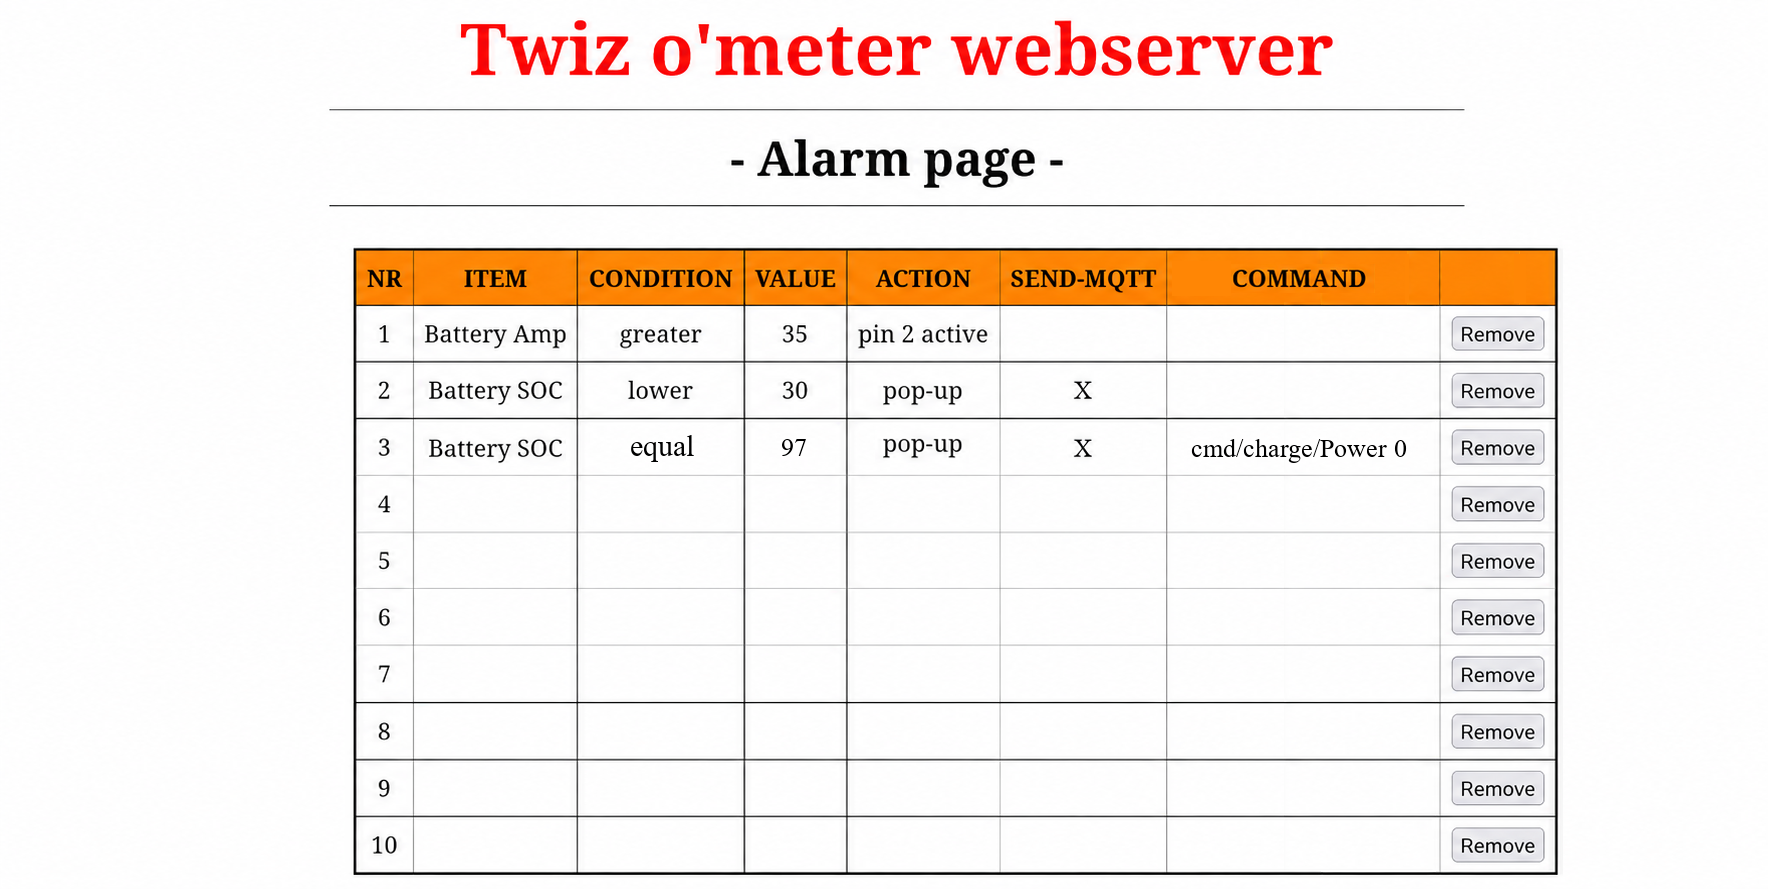
\includegraphics[width=1\textwidth]{figures/alarm_page1.png}
    \caption{Alarmseite --- Liste bestehender Alarme.}
\end{figure}

Die Kopfzeilen der Tabellen sind praktisch die Elemente der Bedingung, auf die ToM+ lauscht.\\

\begin{itemize}
    \item \textbf{ITEM}: Dies sind die zu prüfenden Daten, ausgewählt aus der Liste in Abschnitt~\ref{sec:icon_list}.
    \item \textbf{CONDITION}: Dies ist das Operatorzeichen, das beim Vergleichen der Werte verwendet wird.
    \item \textbf{VALUE}: Dies ist ein vorzeichenbehafteter Ganzzahlwert, der als zweiter Begriff des Vergleichs verwendet wird.
    \item \textbf{ACTION}: Dies ist die Aktion, die ausgeführt wird, wenn der Alarm auslöst. Siehe die nächste Tabelle.
    \item \textbf{SEND-MQTT}: Dies ist ein binäres Feld; wenn es angekreuzt ist, wird eine Nachricht auf dem MQTT-Topic veröffentlicht.
    \item \textbf{COMMAND}: Dies ist eine optionale Zeichenfolge, die als zusätzlicher Befehl gesendet werden kann.
\end{itemize}
\  \\
Der erste Alarmauslöser prüft den Batterieverbrauch und aktiviert PIN2 der Erweiterungsplatine, wenn er größer als 35A ist. In diesem spezifischen Beispiel wird er verwendet, um das hintere Bremslicht einzuschalten, wenn die Rekuperation ausreicht, um den Twizy zu verlangsamen.\\

Der zweite Alarmauslöser prüft den Batterie-SOC und zeigt auf dem Display ein einfaches Pop-up an, das benachrichtigt, dass der Batteriepegel niedriger als 30\% ist. Durch Aktivieren des Feldes \textit{„Change page“} habe ich eine weitere Option hinzugefügt, die ToM+ anweist, eine MQTT-Nachricht zu senden, wenn dieser Alarm auslöst.\\

Der dritte Alarmauslöser prüft den Batterie-SOC und führt nach Abschluss des Ladevorgangs (z.~B. gleich 97\%) dasselbe wie zuvor aus, führt jedoch einen zusätzlichen Befehl aus. Der Befehl \textit{cmd/charge/Power 0} deaktiviert einen Tasmota WLAN-Schalter, der den Twizy-Stecker mit der Wandsteckdose verbindet.

Die Funktion der Spalte \textbf{„COMMAND“} ist also sehr nützlich und ermöglicht es Ihnen, Ihr ToM+ in Ihr IoT-Haus einzubinden. Siehe Anhang~\ref{apx:tasmota} für detaillierte Konfigurationen.\\

Wenn Sie einen bestimmten Alarm entfernen möchten, müssen Sie nur die Schaltfläche \textbf{„Remove“} in der letzten Spalte drücken.\\


\begin{figure}[H]
    \centering
    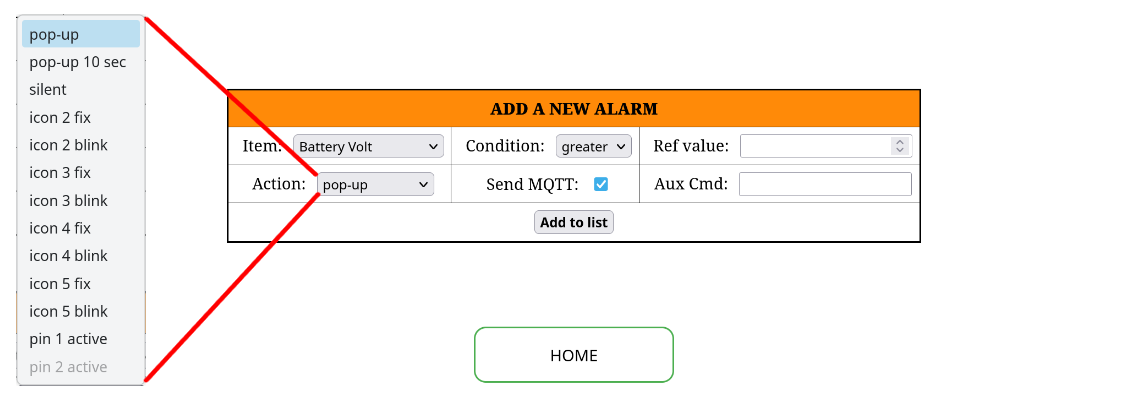
\includegraphics[width=1\textwidth]{figures/alarm_page2.png}
    \caption{Alarmseite --- Tabelle zum Hinzufügen neuer Alarme.}
\end{figure}

In der zweiten Tabelle können Sie der eben besprochenen Liste einen neuen Alarm hinzufügen. Zunächst müssen Sie das \textbf{ITEM} aus allen in Abschnitt~\ref{sec:icon_list} aufgeführten verfügbaren Daten auswählen. In diesem Auswahlfeld sind die Elemente wie in der eben zitierten Liste organisiert. Wählen Sie dann die \textbf{CONDITION}, d.~h. den Operator des Vergleichs, zwischen \textit{„lower“}, \textit{„greater“} oder \textit{„equal“}. Als Nächstes ist der Referenz-\textbf{VALUE} an der Reihe, eine vorzeichenbehaftete Ganzzahl, der rechte Begriff des Vergleichs.\\

Nehmen wir uns etwas Zeit, um alle möglichen \textbf{ACTION}s zu erklären.\\

\begin{itemize}
    \item \textit{pop-up}: Ein gelbes Pop-up, das den Elementwert mitteilt, erscheint in der Mitte des Bildschirms. Um es auszublenden, drücken Sie es einmal. Ein Pop-up-Beispiel sehen Sie im ersten Bild unten.
    \item \textit{pop-up 10 sec}: Ein gelbes Pop-up, das den Elementwert mitteilt, bleibt zehn Sekunden lang auf dem Bildschirm.
    \item \textit{silent}: Es finden keine sichtbaren Aktionen statt: Wird häufig verwendet, um nur MQTT-Nachrichten zu senden.
    \item \textit{icon x fix}: Symbol x (\textit{wobei x 2, 3, 4 oder 5 sein kann}) leuchtet auf. Siehe Abbildung~\ref{fig:alarm_icons2} für Alarmsymbole.
    \item \textit{icon x blink}: Symbol x (\textit{wobei x 2, 3, 4 oder 5 sein kann}) beginnt zu blinken.
    \item \textit{pin1 active}: PIN1 der Erweiterungsplatine wird aktiviert (LOW oder HIGH je nach Pegel, der in den Erweiterungseinstellungen in Abschnitt~\ref{sec:web_alarm_triggers} gewählt wurde).
    \item \textit{pin2 active}: PIN2 der Erweiterungsplatine wird aktiviert. In diesem Beispiel wurde PIN2 als INPUT-Modus eingestellt, ist also ausgegraut, da er keine OUTPUT-Aktion darstellen kann.
\end{itemize}
\  \\
\begin{figure}[ht]
    \centering

    \begin{subfigure}[t]{0.48\textwidth}
        \centering
        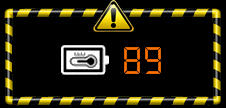
\includegraphics[width=\linewidth]{figures/pop-up.PNG}
        \caption{Pop-up: Batterietemp > 89°C.}
    \end{subfigure}
    \hfill
    \begin{subfigure}[t]{0.48\textwidth}
        \centering
        
\includegraphics[width=\linewidth]{figures/alarm_icons.png}
        \caption{Alarmsymbole (2, 3, 4 und 5).}\label{fig:alarm_icons2}
    \end{subfigure}
\end{figure}

Das nächste Feld ist das binäre \textbf{SEND MQTT}-Flag: Wenn aktiviert, veröffentlicht ToM+ eine MQTT-Nachricht auf dem konfigurierten MQTT-Out-Topic (z.~B. TOMout, siehe Abschnitt~\ref{sec:mqtt_connection}), wenn der Alarm als zusätzliche Benachrichtigung auslöst. Zu guter Letzt gibt es das Textfeld \textbf{AUX CMD}, das einen zusätzlichen Befehl enthält, der über MQTT an andere IoT-Geräte gesendet werden kann. Siehe Anhang~\ref{apx:tasmota} für detaillierte Konfigurationen eines Tasmota-Schalters als Beispiel.\\

Schließlich können Sie Ihren Alarm hinzufügen, indem Sie die Schaltfläche \textbf{„Add to list“} drücken. Die Seite wird automatisch neu geladen und der Alarmauslöser wird an die Liste in der ersten Tabelle angehängt.

Drücken Sie am Ende der Seite die grüne Taste \textbf{„HOME“}, um zur Startseite zurückzukehren.


\subsection{Alarmsystem-Protokollseite}
\label{sec:web_alarms_log}

Diese Seite speichert die letzten 21 Alarmauslösungen und erfüllt dieselbe Funktion wie die Protokollseite von ToM, wie in Abschnitt~\ref{sec:alarm_log} gezeigt. Sie können unerwünschte Datensätze auch anzeigen und entfernen, indem Sie die Schaltfläche \textbf{„Remove“} neben dem Datensatz drücken, den Sie dauerhaft löschen möchten (auch auf dem ToM+-Display).\\

\begin{figure}[H]
    \centering
    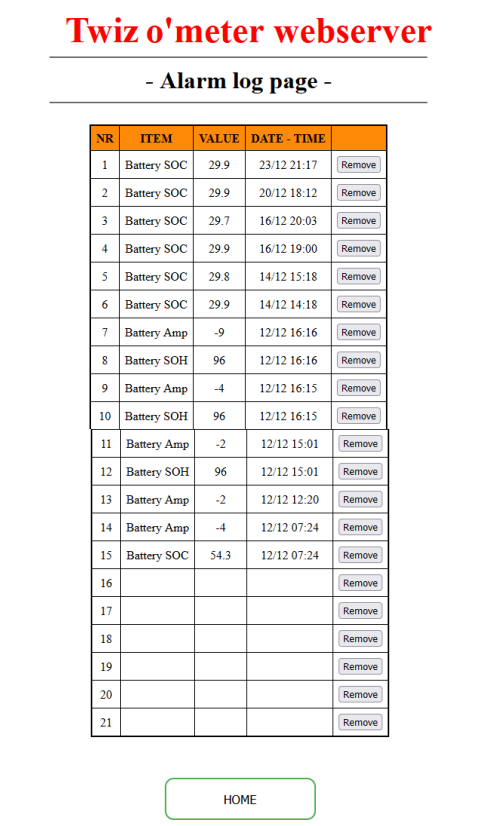
\includegraphics[width=0.6\textwidth]{figures/alarm_log1.png}
    \caption{Tabelle der Alarmlogbuch-Seite.}
\end{figure}

Offensichtlich enthält die Tabelle das \textbf{ITEM} und den \textbf{VALUE}, die den Alarm ausgelöst haben. Es gibt jedoch zusätzliche Felder mit Datum und Uhrzeit, wann die Auslösung stattfand. Drücken Sie dann wie gewohnt am Ende der Seite die grüne Schaltfläche \textbf{„HOME“}, um zur Startseite zurückzukehren.


\subsection{OTA-Update \& Einstellungsseite}
\label{sec:web_ota_update}

Auf dieser Seite können Sie die \textbf{Firmware spontan über die Weboberfläche aktualisieren}, ohne sich wie in älteren Versionen mit dem Flash-Tool herumschlagen zu müssen. Diese neue Funktion spart Zeit und ist viel benutzerfreundlicher. Stellen Sie daher sicher, dass Sie immer die neueste Version der Firmware installiert haben, um Zugriff auf die neuesten Funktionen und Verbesserungen zu haben!

\subsubsection{OTA-Update}

Die erste Tabelle gibt Ihnen einige Informationen über die Blackbox-Firmware: Besprechen wir diese Werte. Die \textbf{ESP fw} ist wahrscheinlich das wichtigste Element im Raster, da sie Ihnen die Version mitteilt, die derzeit auf dem ESP-Motherboard installiert und geladen ist.

Ein weiteres nützliches Feld ist die \textbf{S/N}, die für Seriennummer steht, die Sie auch auf dem ToM+ finden, wie in Abbildung~\ref{fig:settings_page} gesehen. Die nächste Zeile ist etwas technischer und steht in direktem Zusammenhang mit dem OTA-Update-Mechanismus (Over-The-Air). \textbf{Current ptn} und \textbf{Next ptn} beziehen sich auf die Partitionsadressen, an denen die Firmware derzeit gespeichert ist und wo sie während des laufenden Updates gespeichert wird.\\

Manchmal werden Firmware-Patches, wie Fehlerbehebungen oder kleinere Dinge, veröffentlicht, ohne die Versionsnummer zu ändern (z.~B. 2.4). In diesen Fällen kann es nützlich sein zu wissen, welche spezifische Binärdatei installiert ist; daher enthalten die nächsten beiden Felder deren vollständigen Namen. Wie Sie sehen können, gibt es zwei Haupt-Firmware-Partitionen, \textbf{Ota0} und \textbf{Ota1}, sodass Sie zwei verschiedene Versionen installiert haben und bei Bedarf zwischen ihnen wechseln können. Hier lautet der vollständige Name für beide \textit{ESP32\_Fw24\_70\_4error12}.

Das letzte Feld ist der vollständige Name der Firmware der \textbf{Special partition}, bei der es sich um einen zusätzlichen Speicher handelt, der zum Halten von Software Dritter verwendet wird (z.~B. die Tuning-Software Twizy-cfg). Weitere Informationen zum Tuning Ihres Twizy mit Twizy-cfg auf ToM+ finden Sie in Anhang~\ref{apx:tuning}.

\begin{figure}[H]
    \centering
    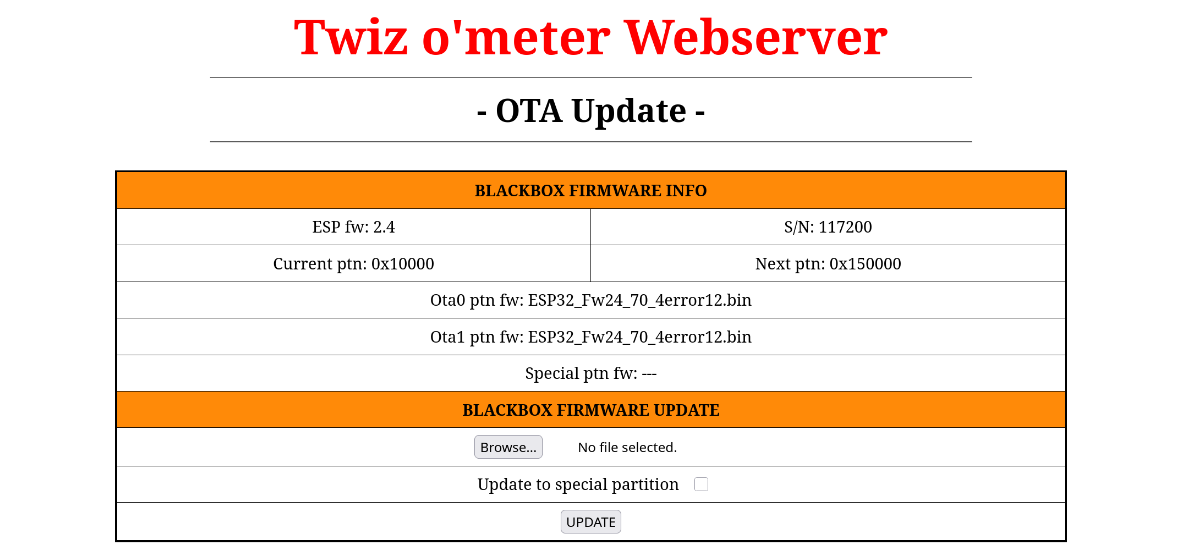
\includegraphics[width=1\textwidth]{figures/ota_page3.png}
    \caption{OTA-Update-Seite --- Update- und Info-Tabelle.}
\end{figure}

Der zweite Teil dieser Tabelle ermöglicht es Ihnen, die Firmware zu aktualisieren oder Software von Drittanbietern zu laden. Laden Sie zunächst die Binärdatei (mit der Endung .bin) herunter, die Sie auf dem ToM+ installieren möchten. Drücken Sie dann die Schaltfläche \textbf{„Browse\ldots“} und navigieren Sie durch Ihre Geräteordner, bis Sie die gewünschte Datei finden.

Wenn es sich um ein \textit{Standard-ToM+-Update} handelt, drücken Sie die Schaltfläche \textbf{„UPDATE“}. Um den Update-Status zu überprüfen, erscheint am unteren Rand der Tabelle ein orangener Fortschrittsbalken mit Prozentangabe. Wenn er 100\% erreicht, startet ToM+ schließlich neu, um die Änderungen zu übernehmen.

Wenn es sich um \textit{Software von Drittanbietern} handelt, stellen Sie sicher, dass Sie die Option \textit{„Update to special partition“} aktivieren und erst danach die Schaltfläche \textbf{„UPDATE“} drücken. Sobald das Update abgeschlossen ist, startet ToM+ neu und lädt die Firmware der Spezialpartition.\\

In der Tabelle \textbf{„BOOT OPTIONS“} können Sie hingegen, sobald Sie die gewünschten Firmwares geladen haben, bei Bedarf zwischen ihnen wechseln. Nehmen wir an, ich nutze die ToM+ 2.4 Firmware und möchte etwas Tuning mit der Drittanbieter-Software Twizy-cfg durchführen; ich habe bereits beide in die korrekten Partitionen geladen. Um dies zu erreichen, drücken Sie die Schaltfläche \textit{„Reboot from special partition“} und warten Sie, bis ToM+ neu startet; folgen Sie dann Anhang~\ref{apx:tuning} für weitere Informationen.\\

Die Schaltflächen \textit{„Reboot from Ota0 partition“} und \textit{„Reboot from Ota1 partition“} werden verwendet, um zwischen den ToM+-Firmware-Versionen zu wechseln. Nehmen wir an, ich nutze die ToM+ 2.4 Firmware, möchte aber aus irgendeinem Grund zur Version 2.3 zurückkehren, die ich zuvor hatte. Drücken Sie dazu die entsprechende Schaltfläche, um entweder von Ota1 oder Ota0 neu zu starten. ToM+ startet sofort neu und die Verbindung zur Weboberfläche wird getrennt.

\begin{figure}[H]
    \centering
    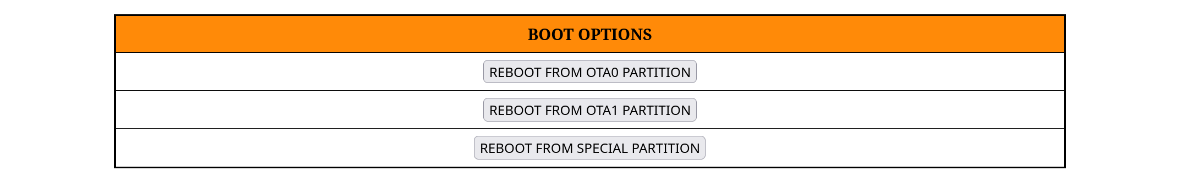
\includegraphics[width=1\textwidth]{figures/ota_boot.png}
    \caption{OTA-Update-Seite --- Tabelle für Boot-Optionen.}
\end{figure}

In der nächsten Tabelle haben wir die Tabelle \textbf{„LCD FIRMWARE UPDATE“}, die es ermöglicht, OTA-Updates auch für das LCD-Display durchzuführen. Das bedeutet kein Hantieren mehr mit der MicroSD-Karte und dem kleinen Loch am Display.\\

\textbf{WARNUNG:} Wie in der Tabelle beschrieben, dürfen Sie diese Webseite während des Updates \textbf{NICHT} schließen: Es wird empfohlen, Ihren Bildschirmschoner zu deaktivieren, um ein Fehlschlagen des Updates zu vermeiden. Der Vorgang kann je nach Firmware-Version einige Minuten dauern, bis zu 10 Minuten.\\

Dies ist ähnlich wie das Blackbox-OTA-Update. Laden Sie also zuerst die Datei (mit der Endung .tft) herunter, die Sie auf dem ToM+ installieren möchten. Drücken Sie dann die Schaltfläche \textbf{„Browse\ldots“} und navigieren Sie durch Ihre Geräteordner, bis Sie die gewünschte Datei finden.

Wenn Sie das \textit{Hauptdisplay aktualisieren}, drücken Sie die Schaltfläche \textbf{„UPDATE LCD“}. Um den Update-Status zu überprüfen, zeigt der blaue Fortschrittsbalken unter dem Haftungsausschluss-Feld die auf das LCD kopierten Blöcke an. Wenn er fertig ist, startet das Display neu (nicht die Blackbox).

Wenn Sie das \textit{Zusatzdisplay (Twin Display) aktualisieren}, stellen Sie sicher, dass Sie die Option \textit{„Update AUX LCD“} aktivieren und erst danach die Schaltfläche \textbf{„UPDATE LCD“} drücken. Sobald das Update abgeschlossen ist, startet das LCD-Display neu und lädt die gewünschte Firmware.

\begin{figure}[H]
    \centering
    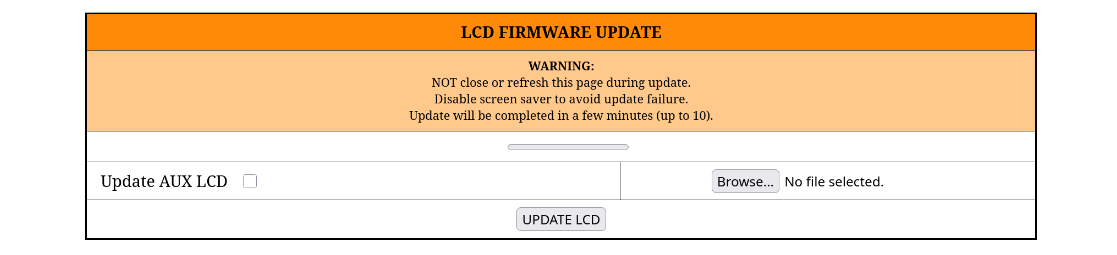
\includegraphics[width=1\textwidth]{figures/ota_lcd.png}
    \caption{OTA-Update-Seite --- Tabelle für LCD-Firmware-Update.}
\end{figure}


\subsubsection{Einstellungen und HW-Upgrade}

Im nächsten Abschnitt der Webseite können wir Einstellungen verwalten, was WLAN- und MQTT-Konfigurationen, Symbolanordnungen der ToM+-Seiten und mehr umfasst. Es ist daher immer ratsam, \textbf{vor dem Update ein Backup} zu erstellen, um die erneute Eingabe von Passwörtern zu vermeiden, falls ein Update fehlschlägt. Drücken Sie dazu die Schaltfläche \textbf{„BACKUP“}, und eine Datei namens \textit{prefs.ToM} wird auf Ihr Gerät heruntergeladen. Manchmal öffnet sich ein Pop-up, um Sie zu warnen, dass diese Datei eine ungewöhnliche Dateiendung hat; klicken Sie auf die Schaltfläche \textit{Behalten} und laden Sie sie trotzdem herunter.\\

Der umgekehrte Vorgang ist ebenso einfach. Drücken Sie die Schaltfläche \textbf{„Browse\ldots“} und navigieren Sie durch Ihre Geräteordner, bis Sie die Einstellungsdatei \textit{prefs.ToM} finden. Um die Änderungen zu übernehmen, drücken Sie die Schaltfläche \textbf{„RESTORE“}; Sie werden zur Bestätigung auf die Startseite weitergeleitet.

\begin{figure}[H]
    \centering
    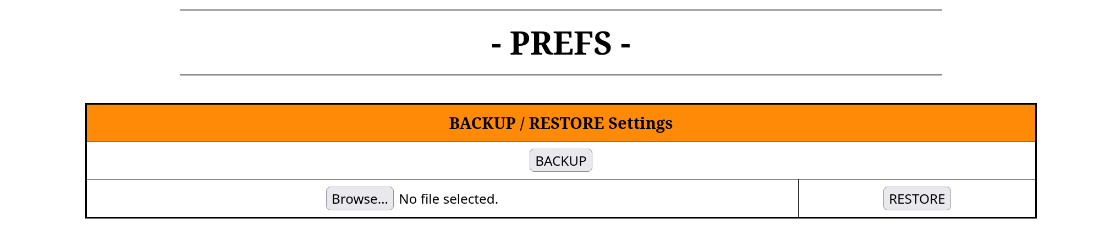
\includegraphics[width=1\textwidth]{figures/prefs_page.png}
    \caption{OTA-Update-Seite --- Tabelle zur Einstellungssicherung.}
\end{figure}

Diese nächste Tabelle ist sehr spezifisch für Benutzer älterer ToM-Versionen, die nun das Passwort erhalten haben, um ihr Gerät auf ToM+ aufzurüsten, ohne die Blackbox auszutauschen. Wenn dies bei Ihnen der Fall ist, geben Sie bitte das Passwort in das Textfeld ein und drücken Sie die Schaltfläche \textbf{„UPGRADE“}. Von nun an ist Ihr ToM endlich auf ToM+ aufgerüstet, viel Spaß!

\begin{figure}[H]
    \centering
    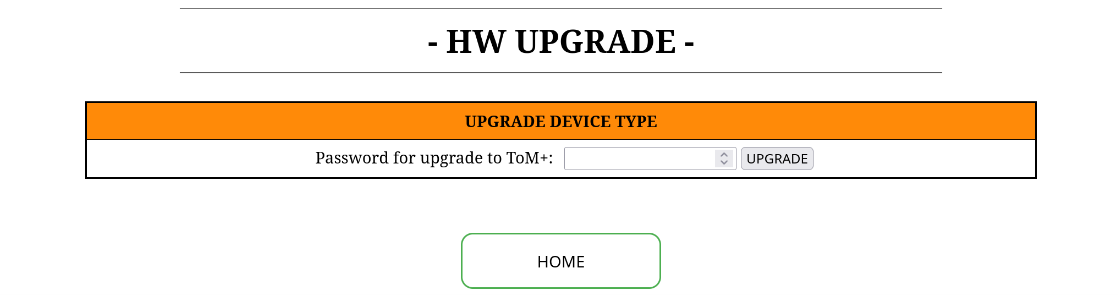
\includegraphics[width=1\textwidth]{figures/hw_upgrade.png}
    \caption{OTA-Update-Seite --- Tabelle zum Hardware-Upgrade.}
\end{figure}

Drücken Sie am Ende der Tabelle die grüne Taste \textbf{„HOME“}, um zur Startseite zurückzukehren.

\clearpage

\subsection{Erweiterte Info- \& Einstellungsseite}
\label{sec:web_advanced_info}

Diese Seite ist für verschiedene erweiterte Einstellungen gedacht, die aus Platzgründen nicht auf den Einstellungsseiten des ToM+-Displays (besprochen in Abschnitt~\ref{sec:settings_page}) verfügbar sind.\\

Das erste Flag, \textbf{„Disable Auto-dimming“}, kann aktiviert werden, wenn Sie nicht möchten, dass das LCD-Display des ToM+ die Helligkeit beim Einschalten des Fernlichts/Abblendlichts anpasst. Andernfalls können Sie die \textbf{„Dimming brightness (\%)“} in Prozent (bis zu 100\%) einstellen und den Faktor der Helligkeitsreduzierung bei Aktivierung der Scheinwerfer selbst festlegen.

\begin{figure}[H]
    \centering
    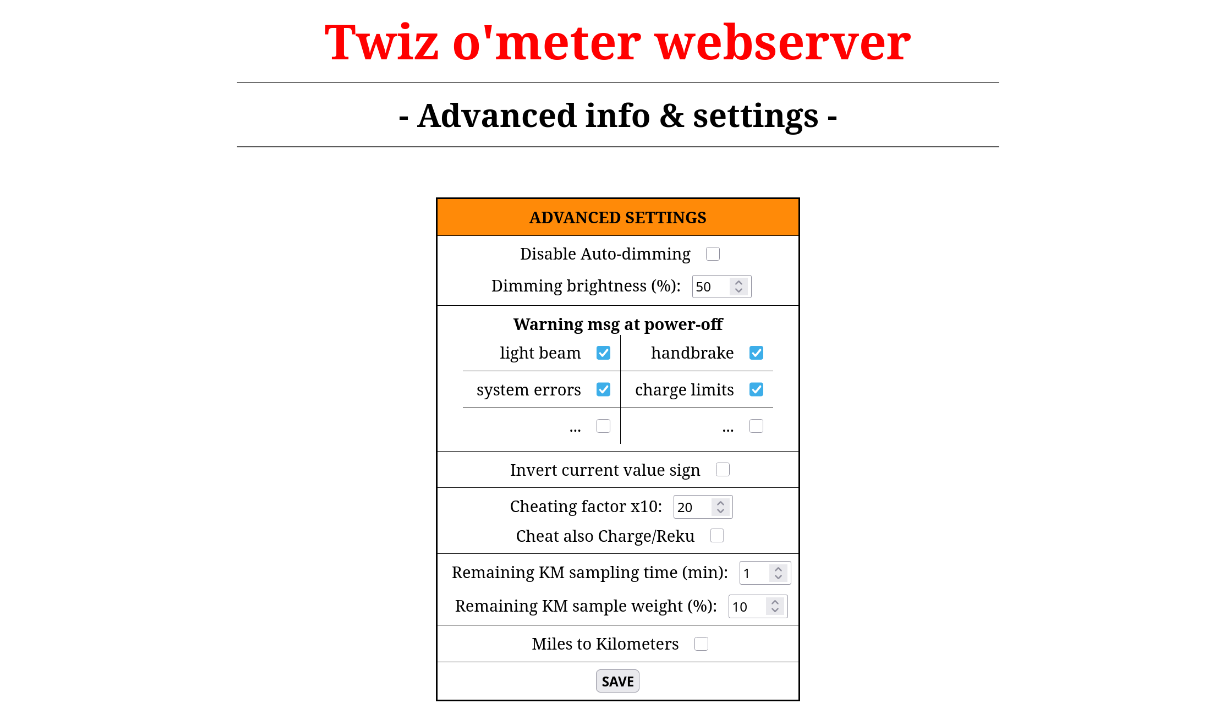
\includegraphics[width=1\textwidth]{figures/adv_sett_page1.png}
    \caption{Erweiterte Info-Seite --- Tabelle für erweiterte Einstellungen.}
\end{figure}

Als Nächstes haben wir den Unterabschnitt \textbf{Warnmeldungen beim Ausschalten}, in dem Sie die Erinnerungen (\textit{Scheinwerfer} und \textit{Handbremse}) und Infos (\textit{Systemfehler} und \textit{Ladebegrenzungen}) auswählen können, die beim Ausschalt-Pop-up des ToM+ angezeigt werden. Es sieht aus wie im Bild unten gezeigt und lässt Sie beispielsweise wissen, wenn Sie vergessen haben, die Handbremse anzuziehen. Die letzten beiden Kontrollkästchen sind für zukünftige Verwendungen reserviert und noch nicht implementiert.

\begin{figure}[H]
    \centering
    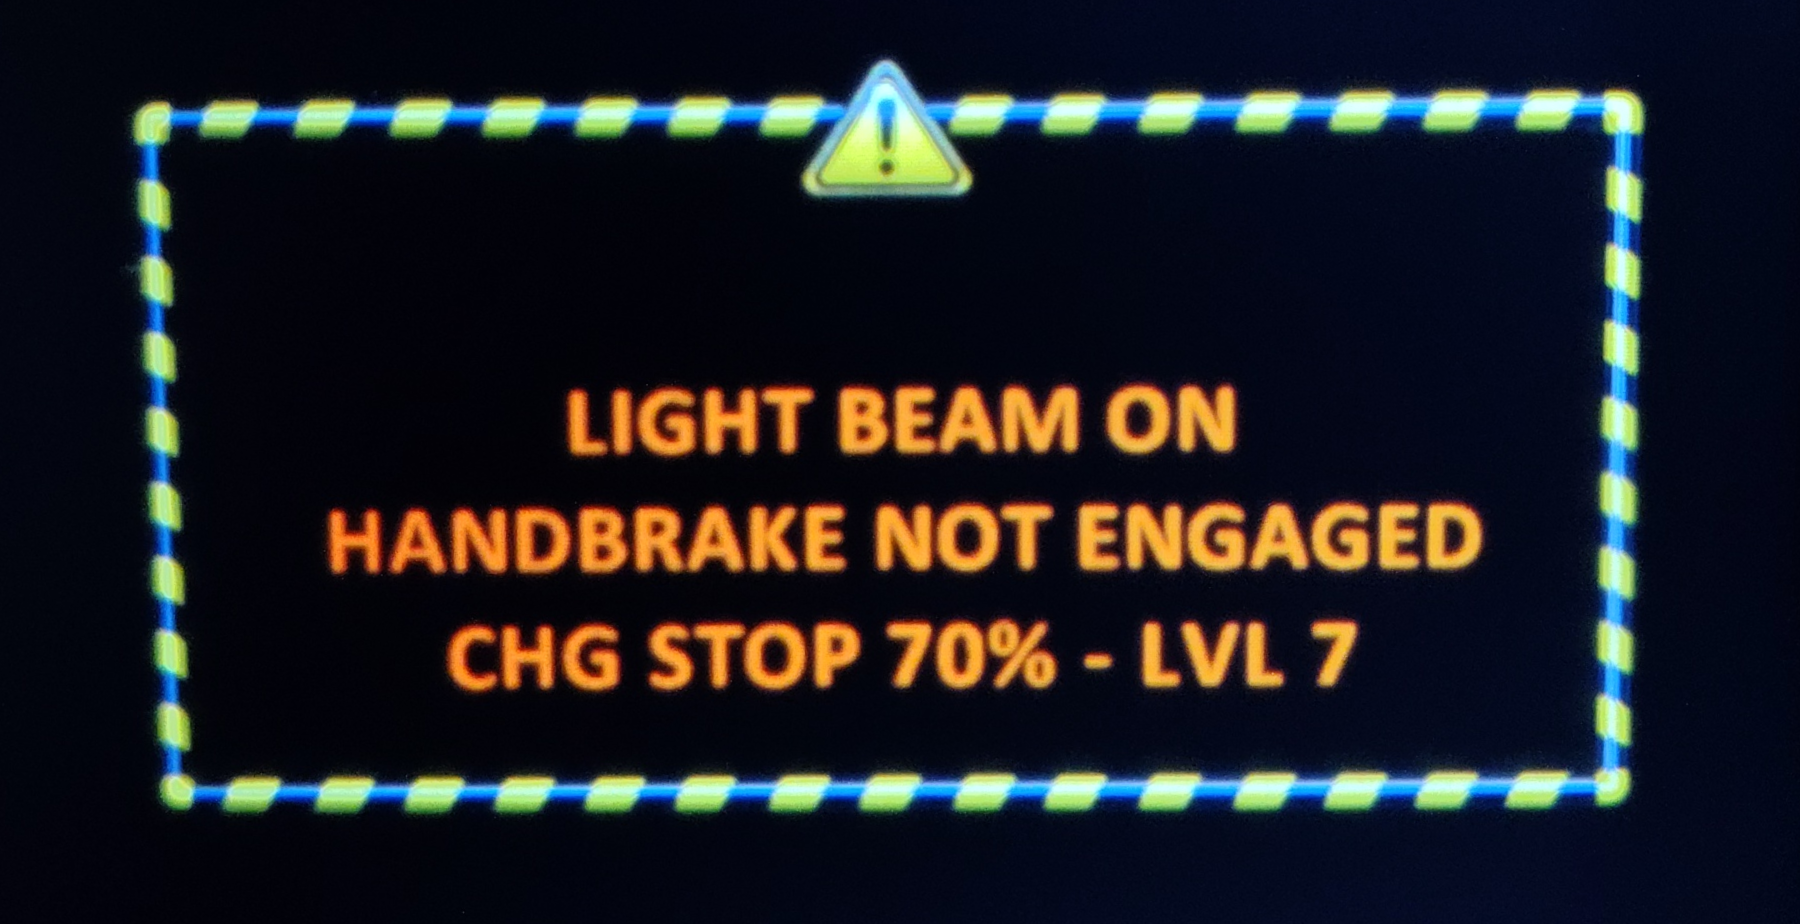
\includegraphics[width=0.5\textwidth]{figures/pop-up_finale.png}
    \caption{Warnmeldung beim Ausschalten.}
\end{figure}

Dann gibt es die \textbf{„Secondary font colour“} mit einer Farbauswahl, mit der die sekundäre Schriftfarbe auf dem ToM+-Display geändert werden kann.

Ein weiteres verfügbares Flag ist \textbf{„Invert current value sign“}. Wenn aktiviert, zeigt es bei den Stromverbrauchswerten im Grunde eine vorzeichenbehaftete Ganzzahl anstelle von Absolutwerten an.\\

Die kleine Untergruppe darunter ist der \textbf{Cheatzy}-Kompatibilität mit ToM+ gewidmet. Sie können Ihren \textbf{„Cheating factor“} multipliziert mit 10 einstellen: Beispielsweise wird 2,0 zu 20. Sie können auch auswählen, ob der Cheatzy beim Laden oder beim regenerativen Bremsen aktiviert ist, indem Sie das Flag \textbf{„Cheat also Charge/Reku“} verwenden. Diese Einstellungen machen nur Sinn, wenn der Cheatzy angeschlossen und eingeschaltet ist; andernfalls können sie Ihre Stromwerte fehlerhaft verändern.\\

Dann gibt es ein weiteres Flag: \textbf{„Increase thermal protection threshold“}, mit dem der Überhitzungsschutz-Schwellenwert für ToM+ in wärmeren Jahreszeiten um 15°C erhöht werden kann.

Die nächsten beiden Werte sind zusätzliche Konfigurationen für die von ToM+ berechneten \textbf{Rest-KM}, basierend auf einer Abtastung des aktuellen Verbrauchs. Hier können Sie im Feld \textbf{„Remaining KM sampling time (min)“} einstellen, wie oft die Abtastung erfolgt (Standard: einmal pro Minute) und wie stark die letzte Stichprobe die Gesamtberechnung beeinflusst (Standard: 10\%) im Feld \textbf{„Remaining KM sample weight (\%)“}.\\

Schließlich haben wir das Flag \textbf{„Miles to Kilometers“}, das hilft, wenn Ihr BigToM aus einem meilenbasierten Dashboard erstellt wurde, Sie aber km/h als Maßeinheit wünschen. Wenn aktiviert, führt ToM+ diese Konvertierung für Sie durch.

Bitte denken Sie daran, Ihre \textbf{Änderungen zu speichern}, indem Sie die Schaltfläche \textbf{„SAVE“} am Ende dieser Tabelle drücken. Wenn Sie dies nicht tun, gehen Ihre Änderungen beim Verlassen der Seite verloren.

\begin{figure}[H]
    \centering
    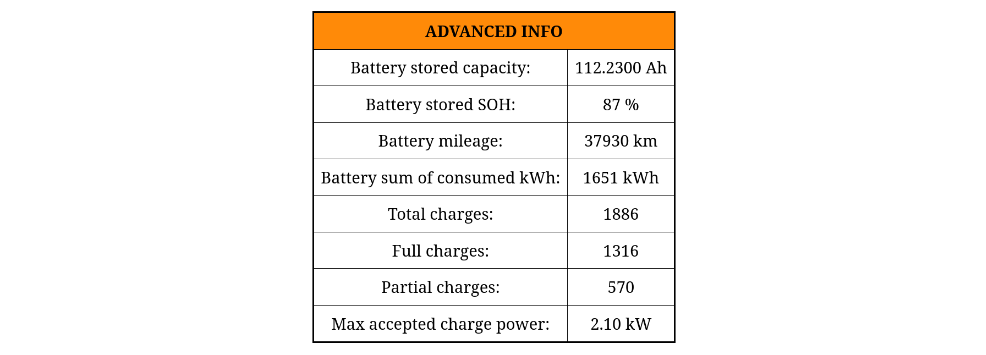
\includegraphics[width=0.9\textwidth]{figures/adv_info.png}
    \caption{Erweiterte Info-Seite --- Tabelle für erweiterte Informationen.}
\end{figure}

Die Tabelle oben enthält Daten zu Ihrer Batterie, wie gespeicherte Kapazität, \textbf{SOH}, \textbf{Batterie-Kilometerstand}, insgesamt verbrauchte kWh und zu Ladevorgängen, wie die Anzahl der \textit{gesamten}, \textit{vollständigen} und \textit{teilweisen} Ladevorgänge sowie die \textbf{maximal akzeptierte Ladeleistung}.\\

\begin{figure}[H]
    \centering
    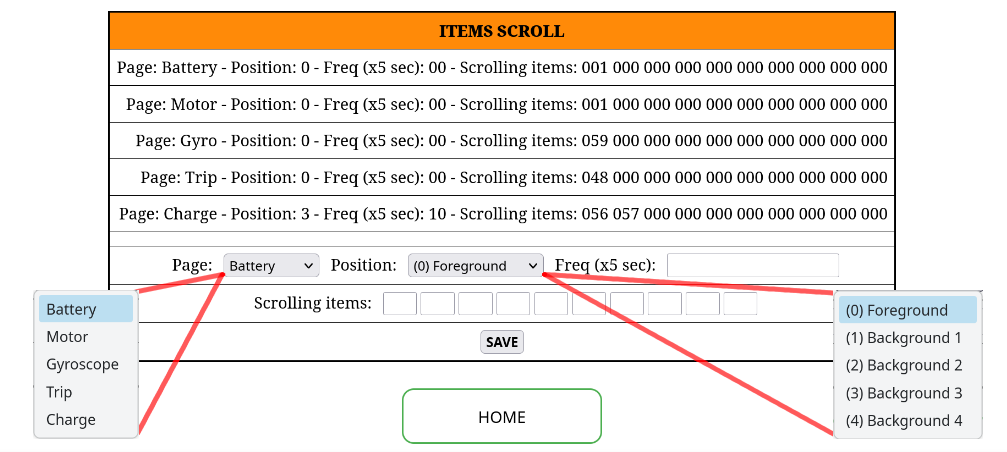
\includegraphics[width=1\textwidth]{figures/item_scroll.png}
    \caption{Erweiterte Info-Seite --- Element-Scroll-Tabelle.}
\end{figure}

Diese letzte Tabelle ist eine sehr spezielle Funktion, die vor einigen Updates eingeführt wurde und es Ihnen ermöglicht, dynamisch wechselnde Elemente auf Seiten Ihrer Wahl zu haben. Sie kann auf die Seiten \textit{Batterie}, \textit{Motor}, \textit{Gyroskop}, \textit{Fahrt} und \textit{Ladevorgang} angewendet werden, und Sie können über das Feld \textbf{„Page“} auswählen, welche davon genutzt werden soll.

Anschließend können Sie auswählen, an welcher Position die Datenelemente Ihrer Wahl gescrollt werden sollen. Verwenden Sie dazu das Feld \textbf{„Position“} und wählen Sie aus der Liste die von Ihnen bevorzugte Position unter Bezugnahme auf Abbildung~\ref{fig:icon_arrangement} für das Layout-Arrangement.\\

Das Feld \textbf{„Freq“} ist die Scrollfrequenz, im Grunde wie lange jedes Datum an dieser Position bleibt, bevor es zum nächsten wechselt. Wie Sie vielleicht bemerken, ist in Klammern angegeben, dass das Feld mit \textit{5 Sekunden} multipliziert wird. Das bedeutet, dass die Eingabe des Werts \textit{1} zu einer Frequenz von \textit{5 Sekunden} führt, der Wert \textit{2} zu einer von \textit{10 Sekunden} und so weiter.

Der wichtigste Teil ist die Auswahl der zu scrollenden Elemente, und Sie können bis zu zehn Datenwerte auswählen. Tragen Sie in den Textbereichen \textbf{„Scrolling items“} die Liste der gewünschten Elementnummern ein (z.~B. 59 oder 48), eine pro Zeile, bezogen auf die Nummern in Klammern in der Liste von Abschnitt~\ref{sec:item_numbers}.\\

Denken Sie immer daran, Ihre Änderungen zu speichern, indem Sie die Schaltfläche \textbf{„SAVE“} am Ende dieser Tabelle drücken. Wenn Sie dies nicht tun, gehen Ihre Änderungen beim Verlassen der Seite verloren.

Wenn Sie die Scroll-Funktion für eine bestimmte Seite und Position \textbf{deaktivieren} möchten, wählen Sie diese Felder aus und geben Sie dann \textit{0} in das Textfeld \textbf{„Freq“} ein. Drücken Sie direkt danach \textbf{„SAVE“}, und das Scrollen wird deaktiviert, wobei zu den Standardwerten zurückgekehrt wird.

Drücken Sie die grüne Taste \textbf{„HOME“} am Ende der Tabelle, um zur Startseite zurückzukehren.



\subsection{Ladeeinstellungen \& Log}
\label{sec:web_charging_prefs}

Diese Seite ist in zwei Haupttabellen unterteilt: Die erste dient zur Steuerung des Ladevorgangs, während die zweite eine Liste der letzten 15 Ladevorgänge mit einigen zusätzlichen Daten enthält.

\subsubsection{Ladeeinstellungen}

Beginnend mit den nützlichsten haben wir das Feld \textbf{„Charging status“}, das Informationen über den aktuellen Status des Fahrzeugs enthält, einschließlich \textit{220V Netz} und \textit{Ladevorgang} mit ihren EIN- und AUS-Flags.

Direkt darunter befindet sich das Feld \textbf{„Charge power limit“}, in dem Sie wählen können, wie viel Leistung Ihr Twizy beim Laden nutzen kann, von $0,4 kW$ bis zu $2,3 kW$ mit 7 Stufen zur Auswahl (wählen Sie \textit{0, um das Leistungslimit zu deaktivieren}).

In der oberen rechten Ecke befindet sich die Schaltfläche \textbf{„ABORT CHARGING“}, die den Ladevorgang sofort und geordnet stoppt, genau wie die auf dem ToM+-Display auf der Einstellungsseite, die wir in Abschnitt~\ref{sec:settings_page} besprochen haben.

\begin{figure}[H]
    \centering
    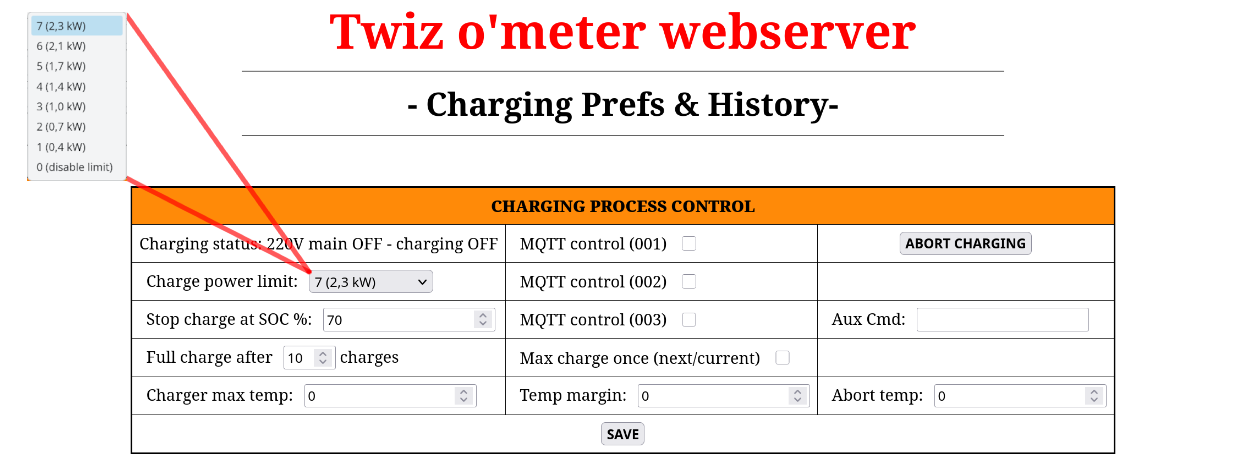
\includegraphics[width=1\textwidth]{figures/charging_process.png}
    \caption{Ladeeinstellungs-Seite --- Tabelle zur Steuerung des Ladevorgangs.}
\end{figure}

Gleich danach befindet sich das Feld \textbf{„Stop charge at SOC \%“}, das den Lade-Prozentsatz angibt, bei dem ToM+ automatisch das Signal zum Abbrechen des Ladevorgangs sendet. Nur zu Ihrer Information: Das Begrenzen der maximalen Ladereihe (95\% oder weniger) verlangsamt den Zerfall des Batterie-SOH.

Weiter zum nächsten Feld haben wir das Feld \textbf{„Full charge after“}, das sich eng auf das letzte bezieht, das wir besprochen haben. Im Grunde stoppt dies den Ladevorgang bei dem ausgewählten SOC einmal alle \textit{X} Ladevorgänge nicht (\textit{zum Beispiel 10} wie im Bild). Denken Sie daran, dass eine 100\%-Ladung hin und wieder hilfreich ist, um die Spannungen der Batteriezellen neu zu balancieren.

Ein weiteres verwandtes Feld ist das Flag \textbf{„Max charge once (next/current)“}, das wie eine Schaltfläche funktioniert und ToM+ anweist, eine vollständige Ladung ohne den gewählten SOC-Stopp durchzuführen. Dies überschreibt das vorherige Feld und wird \textbf{nach dem Drücken von „SAVE“} auf den aktuellen Ladevorgang angewendet, wenn dieser bereits läuft, oder auf den nächsten, falls nicht.\\


Jetzt gibt es ein Sicherheitsfeld, die \textbf{„Charger max temperature“}, in dem Sie einen Schwellenwert (Ganzzahlwert in °C) einstellen können; wird dieser mit einer vom Benutzer definierten Marge-Hysterese überschritten, reduziert ToM+ langsam die zuvor gesehene Leistungsgrenze. Es reduziert diese weiter (bei Bedarf um zwei Stufen), bis die Temperatur wieder normal ist, woraufhin auch die Leistungsgrenze zurückgesetzt wird.

Die genannte Marge ist im entsprechenden Feld \textbf{„Temp margin“} anpassbar, in das Sie einen Ganzzahlwert (in °C) eingeben können, der zur maximalen Ladegerättemperatur addiert wird, um den Schwellenwert zu lockern, bevor die Ladeleistung reduziert wird.

Ein weiteres verwandtes Feld ist die \textbf{„Abort temperature“}, die den letzten Sicherheitsschwellenwert für die Ladegerättemperatur enthält; wird dieser überschritten, bricht ToM+ den Ladevorgang sofort ab.\\


Als Nächstes haben wir drei MQTT-Steuerfelder, die durch ihre fortlaufende Nummer unterschieden werden. Durch Aktivieren eines dieser Flags können Sie den Parameter auf der linken Seite aus der Ferne über das MQTT-Protokoll konfigurieren. Um dies zu erreichen, müssen Sie nach dem Aktivieren des entsprechenden Feldes und dem \textbf{Drücken von „SAVE“} lediglich eine MQTT-Nachricht auf dem in Klammern angegebenen Topic (z.~B. \textit{001} oder \textit{002}) auf Ihrem Broker veröffentlichen (konfiguriert in Abschnitt~\ref{sec:mqtt_connection}).

Wenn Sie die \textbf{MQTT control (001)} aktivieren, können Sie den Ladevorgang starten und stoppen, indem Sie entweder \textit{0} oder \textit{1} auf dem MQTT-Topic \textit{001} veröffentlichen. Das Gleiche gilt für \textbf{MQTT control (002)} durch Veröffentlichung eines Werts zwischen \textit{0} und \textit{7} auf \textit{002} sowie \textbf{MQTT control (003)} auf \textit{003} mit einem Wert zwischen \textit{0} und \textit{100}.\\

Zu guter Letzt haben wir das Feld \textbf{„Aux Cmd“}, das für Zusatzbefehl steht und sich genauso verhält wie das, das wir bereits auf der Alarmauslöser-Seite in Abschnitt~\ref{sec:web_alarm_triggers} besprochen haben. Es wird gesendet, wenn der Ladevorgang abgeschlossen ist oder wenn der Ladevorgang beim angegebenen SOC stoppt.\\


Nach jeder Änderung drücken Sie die Schaltfläche \textbf{„SAVE“}, um \textit{Ihre Änderungen zu speichern}; andernfalls gehen sie beim Verlassen der Seite verloren.

\subsubsection{Ladehistorie}

Die Ladehistorie-Tabelle enthält die letzten fünfzehn Ladevorgänge zusammen mit einigen nützlichen Werten zu deren Bereicherung. Wie Sie sehen können, gibt es Datum und Uhrzeit sowie den \textbf{ODO Kilometers}-Wert beim Start des Ladevorgangs. Daneben sehen wir, wie viel Zeit der Ladevorgang in Anspruch genommen hat, die \textbf{Average Power} (durchschnittliche Leistung) sowie die \textbf{charged kWh} (geladene kWh). Schließlich haben wir \textit{init SOC} und \textit{end SOC}, welche die Start- und Endprozentsätze darstellen.\\


Die letzte Spalte enthält einige zusätzliche \textbf{Notes} (Hinweise) zum Ladestatus, z.~B. wie er gestoppt wurde (entweder Stopp-SOC erreicht oder manuell abgebrochen) oder ob er noch läuft.

Wenn Sie möchten, können Sie auch einige Datensätze manuell löschen, indem Sie die Schaltfläche \textit{X} am Ende des gewünschten Datensatzes drücken. Es ist möglich, alle auf einmal zu löschen, indem Sie die Schaltfläche \textbf{„CLEAR HISTORY“} im unteren Teil der Tabelle drücken.


\begin{figure}[H]
    \centering
    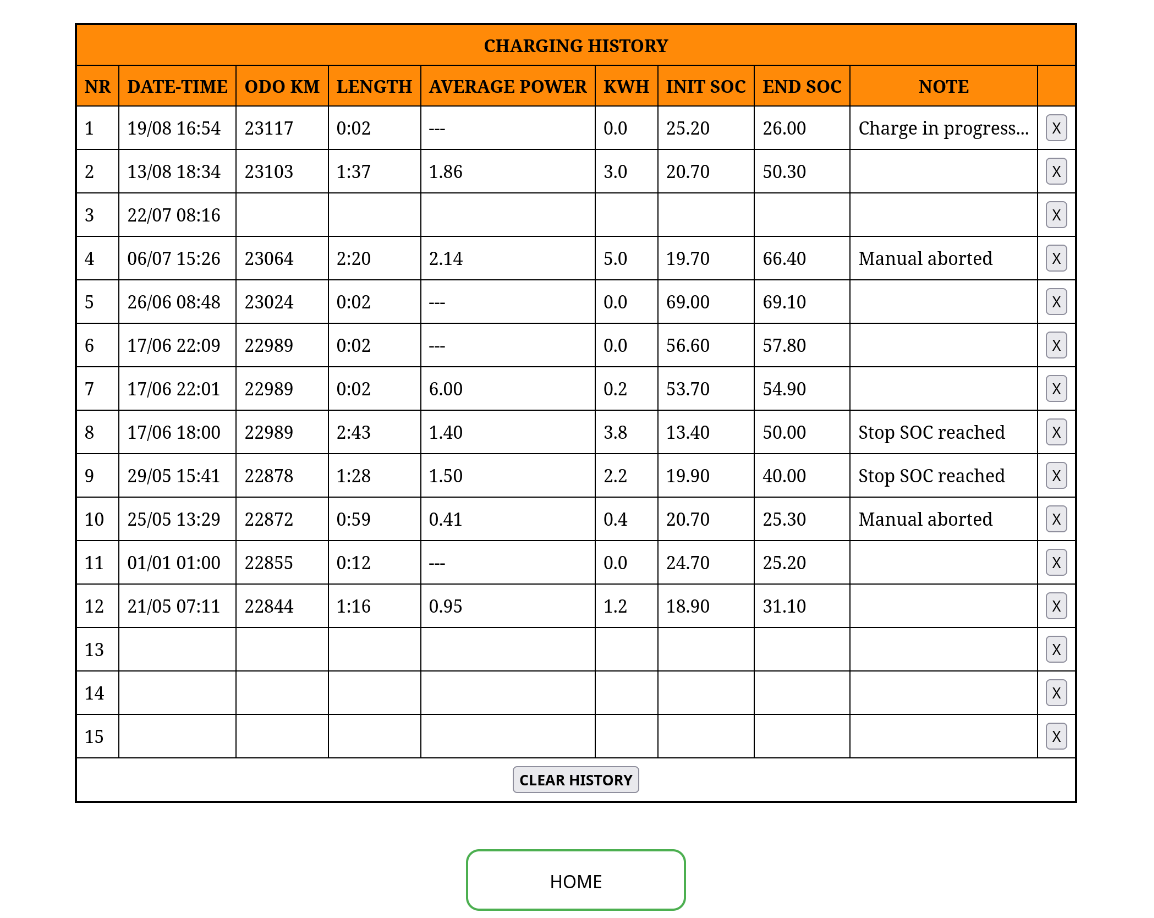
\includegraphics[width=0.95\textwidth]{figures/charging_history.png}
    \caption{Ladeeinstellungs-Seite --- Ladehistorie-Tabelle.}
\end{figure}

Drücken Sie die grüne Taste \textbf{„HOME“} unter der letzten Tabelle, um zur Startseite zurückzukehren.

\clearpage

\subsection{Uhrzeit- \& Datumsseite}
\label{sec:web_time_date}

Mit Ihrem ToM+ können Sie das aktuelle Datum und die Uhrzeit überprüfen, aber wie stellt man sie ein? Diese Seite wurde genau für diesen Zweck erstellt und enthält eine einzelne Tabelle, die im folgenden Bild gezeigt wird.

\begin{figure}[H]
    \centering
    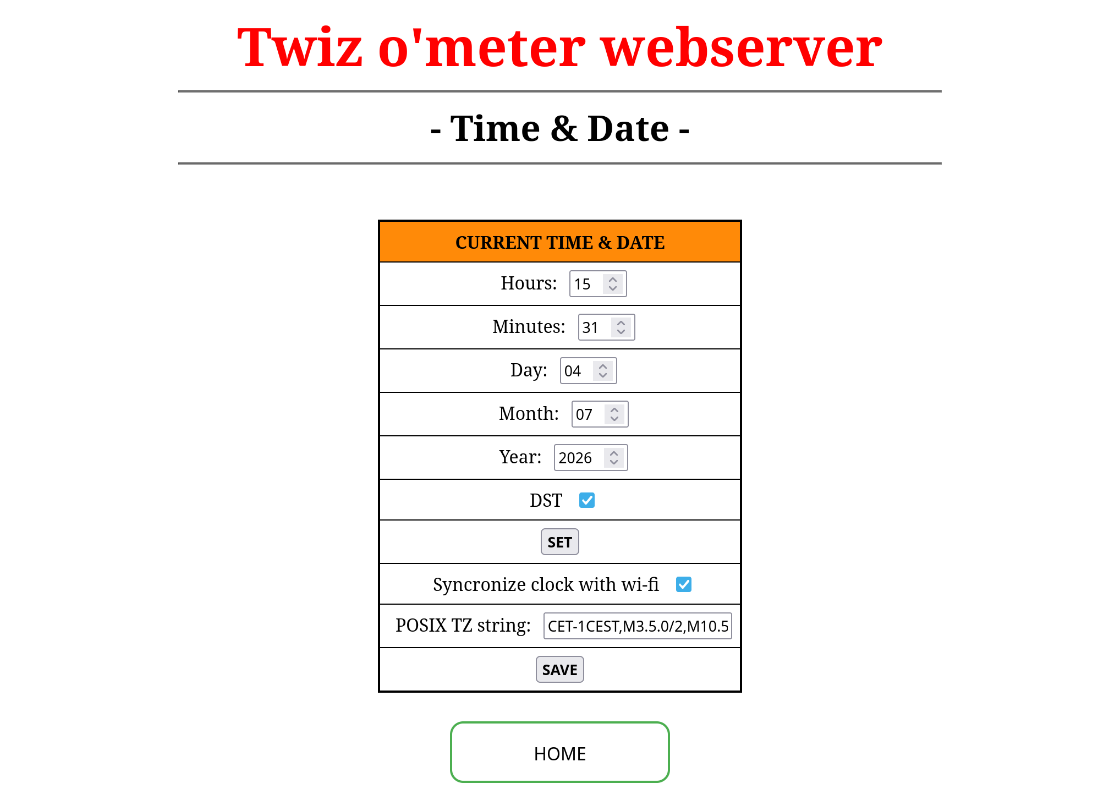
\includegraphics[width=1\textwidth]{figures/time_page.png}
    \caption{Aktuelle Uhrzeit- \& Datumstabelle.}
\end{figure}

Die ersten fünf Felder sind selbsterklärend und intuitiv; passen Sie Datum und Uhrzeit einfach an Ihre Zeitzone an. Das Kontrollkästchen \textbf{„DST“}, das für Daylight Saving Time (Sommerzeit) steht, ermöglicht das Aktivieren oder Deaktivieren des 1-Stunden-Versatzes je nach aktueller Jahreszeit.

Wenn Sie Ihre Änderungen bestätigen und auf ToM+ anwenden möchten, drücken Sie einfach die Schaltfläche \textbf{„SET“}, und sie werden aktualisiert.\\

Als Nächstes haben wir ein sehr nützliches Feld, das Flag \textbf{„Synchronize clock with WiFi“}, das nützlich ist, wenn Sie bereits eine WLAN-Verbindung wie in Abschnitt~\ref{sec:add_wifi_profile} besprochen konfiguriert haben. Schalten Sie dies einfach ein und überlassen Sie ToM+ die Arbeit.

Direkt darunter befindet sich ein technischerer Wert bezüglich des Datums/der Uhrzeit, der ToM+ Ihre aktuelle Zeitzone (\textbf{TZ}) mithilfe einer Zeichenfolge namens \textbf{„POSIX“} mitteilt. Dies beinhaltet auch, wann der 1-Stunden-Sommerzeitversatz angewendet wird. In den meisten mitteleuropäischen Ländern lautet die Zeichenfolge wie folgt: \textit{CET-1CEST,M3.5.0/2,M10.5.0/3}; suchen Sie im Zweifelsfall online nach der POSIX-TZ-Zeichenfolge Ihres Landes.\\


Denken Sie wie immer daran, Ihre Änderungen durch Drücken der Schaltfläche \textbf{„SAVE“} am Ende der Tabelle zu speichern; andernfalls gehen sie beim Verlassen der Seite verloren.

Drücken Sie die grüne Taste \textbf{„HOME“} unter der Tabelle, um zur Startseite zurückzukehren.

\clearpage

\subsection{BigToM / ToM+ Einstellungsseite}
\label{sec:web_btom_tom_sets}

Auf dieser Seite können Sie einige Parameter Ihres BigToM oder ToM+ anpassen, da diese Seite hauptsächlich Konfigurationen für die \textbf{Dashboard-Seite} enthält, die nur auf diesen beiden Geräten verfügbar ist.

\begin{figure}[H]
    \centering
    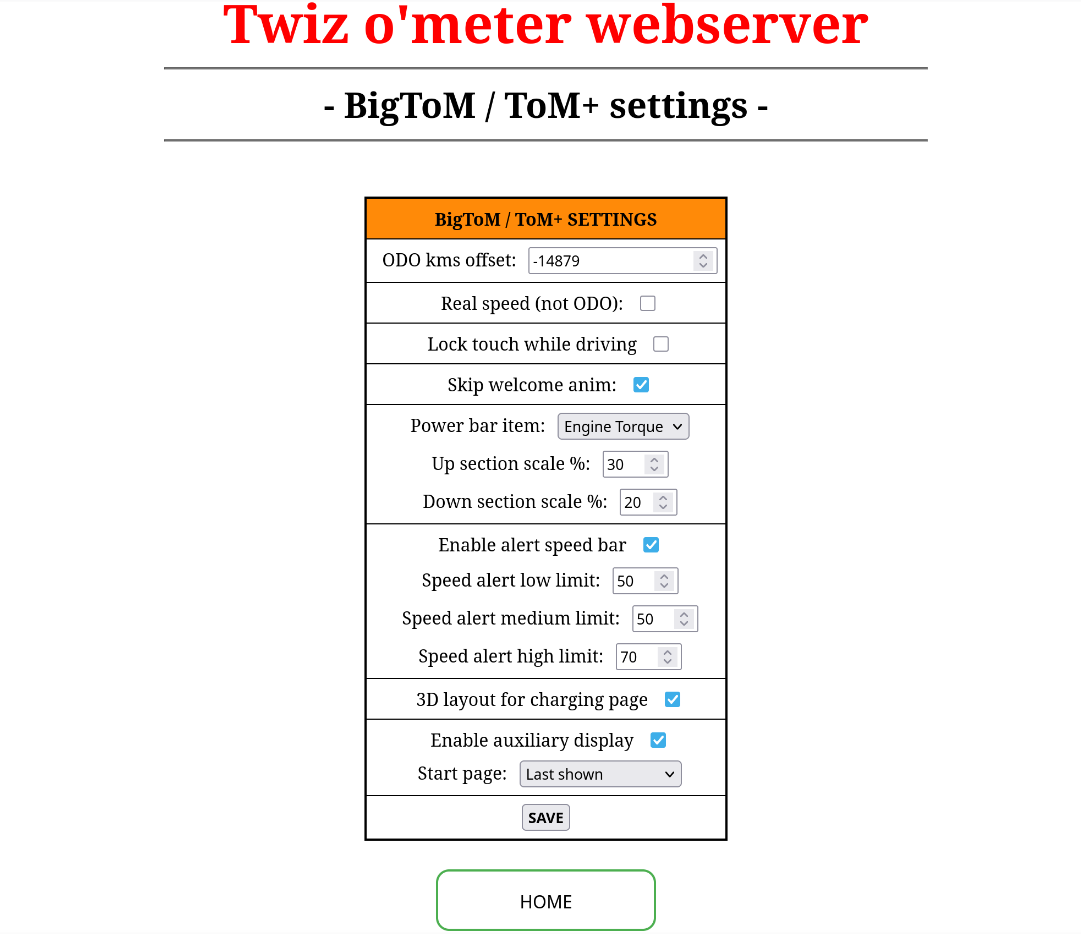
\includegraphics[width=1\textwidth]{figures/btom_page.png}
    \caption{BigToM \textbackslash ToM+ Einstellungstabelle.}
\end{figure}

Beim Ersetzen Ihres Dashboards durch ein BigToM-Dashboard müssen Sie möglicherweise einige Kilometer zum ODO des neuen Dashboards hinzufügen oder davon abziehen, um Ihren ursprünglichen Stand zu erhalten. Das liegt daran, dass sie auf dem Dashboard-Motherboard gespeichert sind. Der erste Parameter ist daher das Feld \textbf{„ODO kms offset“}, das zur Korrektur dieser Kilometerdifferenz verwendet wird.

Wie Sie vielleicht wissen, werden Dashboard-Geschwindigkeitsanzeigen aus Sicherheitsgründen absichtlich um $3 km/h$ erhöht. Wenn Sie Ihre reale Geschwindigkeit sehen möchten, aktivieren Sie einfach das Flag \textbf{„Real speed (not ODO)“} in der zweiten Zeile der Tabelle.\\

Schauen wir uns nun das Flag \textbf{„Lock touch while driving“} an. Wenn aktiviert, wird der Touchscreen während der Fahrt (d.~h. Geschwindigkeit $>0$) aus Sicherheitsgründen deaktiviert.

Als Nächstes haben wir das Flag \textbf{Skip welcome animation}, das aktiviert werden kann, wenn Sie es leid sind, die Begrüßungsanimation beim Wechsel vom Dashboard zu einer anderen Seite zu sehen.\\


Dann gibt es einen Bereich, der dem Leistungsbalken gewidmet ist, der in Abbildung~\ref{fig:dashboard_layout} oben im Dashboard-Layout gezeigt wird. Hier können Sie über das Auswahlfeld \textbf{„Power bar item“} wählen, welcher Wert angezeigt und zum Füllen des Leistungsbalkens verwendet werden soll. Es stehen drei verfügbare Daten zur Auswahl: \textit{Engine Torque} (Motordrehmoment), \textit{Battery Ampere} (Batteriestrom) oder \textit{Battery kW} (Batterieleistung).

Die beiden Felder \textbf{„Up/Down section scale \%“} darunter werden verwendet, um den Bereich des Leistungsbalkens anzupassen, und repräsentieren den Prozentsatz des Maximal-/Minimalwerts des ausgewählten Datenelements. Im Beispielbild habe ich für den maximalen Bereich \textit{30\%} eingetragen.\\


Im nächsten Abschnitt können wir eine weitere nützliche Funktion aktivieren, die ebenfalls in Abbildung~\ref{fig:dashboard_layout} direkt unter der Geschwindigkeitsanzeige gezeigt wird. Dies wird durch Aktivieren des Flags \textbf{„Enable alert speed bar“} erreicht, das über drei anpassbare Schwellenwerte verfügt, die jeweils einer Farbe von \textit{Grün} über \textit{Gelb} bis \textit{Rot} entsprechen.

Die folgenden drei Felder, \textbf{„Speed alert low/medium/high limit“}, sind mit der jeweiligen Schwellenwertgeschwindigkeit in $km/h$ auszufüllen, um die Geschwindigkeitsleiste mit der entsprechenden Farbe aufleuchten zu lassen. Im Beispiel wird die Leiste beim Überschreiten von $50 km/h$ gelb und beim Überschreiten von $70 km/h$ rot. Wie Sie vielleicht bemerken, wollte ich nicht, dass die grüne Leiste angezeigt wird, daher habe ich den Schwellenwert \textit{low} auf denselben Wert wie den Schwellenwert \textit{medium} gesetzt.\\


Vorletztes haben wir das standardmäßig aktivierte Flag \textbf{„3D layout for charging page“}, das 3D-Details anstelle der Standard-ToM-Ladeseite anzeigt.

Und schließlich gibt es die zuletzt hinzugefügte Funktion namens \textbf{Twin ToM}, die für die ursprünglichen ToM-Besitzer entwickelt wurde, bevor ToM+ herauskam. Damit können Sie das kleinere Display zusammen mit der neuen Ansteckversion verwenden, um zwei Seiten gleichzeitig zu überwachen. Damit dies funktioniert, müssen Sie das Flag in der letzten Zeile aktivieren: \textbf{„Enable auxiliary display“}.

Anschließend können Sie über das Auswahlfeld \textbf{„Start page“} eine bestimmte Seite auswählen, die beim Einschalten auf dem Zusatzdisplay angezeigt werden soll, oder einfach \textit{Last shown} (Zuletzt angezeigt) wählen.\\


Denken Sie wie immer daran, Ihre Änderungen durch Drücken der Schaltfläche \textbf{„SAVE“} am Ende der Tabelle zu speichern; andernfalls gehen sie beim Verlassen der Seite verloren.

Drücken Sie die grüne Taste \textbf{„HOME“} unter der Tabelle, um zur Startseite zurückzukehren.

\clearpage

\subsection{Diagnose-Seite}
\label{sec:web_diagnostic}

Diese Seite besteht aus nur einer Tabelle und ermöglicht es Ihnen, weitere Informationen zu den letzten 10 Fehlern anzuzeigen, die in Ihrem Twizy aufgetreten sind, ähnlich wie auf der in Abschnitt~\ref{sec:error_page} besprochenen ToM+-Displayseite.

Die angezeigten Werte sind die \textbf{„DTC Number“} und, falls verfügbar, die \textbf{„DF Number“}, bei denen es sich um eindeutige Identifikatoren für Twizy-Fehler handelt, sodass Sie online danach suchen können. Als Nächstes haben wir den Fehler-\textbf{„Status“}, wie z.~B. \textit{SAVED}, wenn er bereits aufgetreten ist, oder \textit{PRESENT}, wenn er gerade erst aufgetreten ist.

Informationen zur \textit{Aktivierung von DF-Nummern} finden Sie in Abschnitt~\ref{sec:add_wifi_profile}.

\begin{figure}[H]
    \centering
    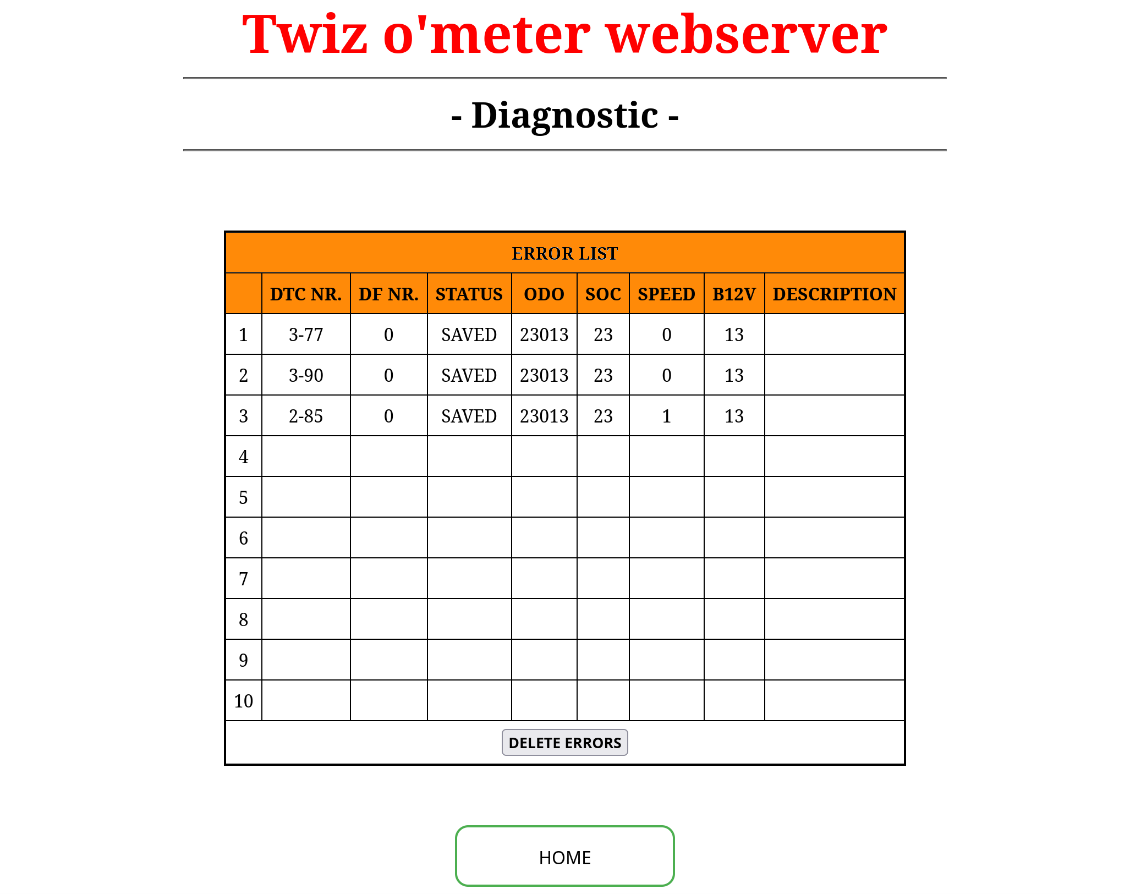
\includegraphics[width=1\textwidth]{figures/error_page.png}
    \caption{Diagnose-Seite --- Fehlerlisten-Tabelle.}
\end{figure}

Zusammen mit diesen Werten sind die nächsten vier Werte die Referenzen für \textbf{„ODO“}, \textbf{„SOC“}, \textbf{„speed“} (Geschwindigkeit) und \textbf{„12V Battery voltage“} (12V-Batteriespannung) zum Zeitpunkt des Auftretens des entsprechenden Fehlers.

Für jeden Fehlerdatensatz gibt es, falls verfügbar, ein Feld für die Fehler-\textbf{„Description“} (Beschreibung).\\


Wenn Sie Twizy-Fehler löschen möchten, selbst fatale, können Sie die unten stehende Schaltfläche \textbf{„DELETE ERRORS“} drücken, die alle Fehler auf einmal löscht.

Drücken Sie die grüne Taste \textbf{„HOME“} unter der Tabelle, um zur Startseite zurückzukehren.